% Options for packages loaded elsewhere
\PassOptionsToPackage{unicode}{hyperref}
\PassOptionsToPackage{hyphens}{url}
%
\documentclass[
]{book}
\usepackage{lmodern}
\usepackage{amsmath}
\usepackage{ifxetex,ifluatex}
\ifnum 0\ifxetex 1\fi\ifluatex 1\fi=0 % if pdftex
  \usepackage[T1]{fontenc}
  \usepackage[utf8]{inputenc}
  \usepackage{textcomp} % provide euro and other symbols
  \usepackage{amssymb}
\else % if luatex or xetex
  \usepackage{unicode-math}
  \defaultfontfeatures{Scale=MatchLowercase}
  \defaultfontfeatures[\rmfamily]{Ligatures=TeX,Scale=1}
\fi
% Use upquote if available, for straight quotes in verbatim environments
\IfFileExists{upquote.sty}{\usepackage{upquote}}{}
\IfFileExists{microtype.sty}{% use microtype if available
  \usepackage[]{microtype}
  \UseMicrotypeSet[protrusion]{basicmath} % disable protrusion for tt fonts
}{}
\makeatletter
\@ifundefined{KOMAClassName}{% if non-KOMA class
  \IfFileExists{parskip.sty}{%
    \usepackage{parskip}
  }{% else
    \setlength{\parindent}{0pt}
    \setlength{\parskip}{6pt plus 2pt minus 1pt}}
}{% if KOMA class
  \KOMAoptions{parskip=half}}
\makeatother
\usepackage{xcolor}
\IfFileExists{xurl.sty}{\usepackage{xurl}}{} % add URL line breaks if available
\IfFileExists{bookmark.sty}{\usepackage{bookmark}}{\usepackage{hyperref}}
\hypersetup{
  pdftitle={Matemàtiques II},
  hidelinks,
  pdfcreator={LaTeX via pandoc}}
\urlstyle{same} % disable monospaced font for URLs
\usepackage{color}
\usepackage{fancyvrb}
\newcommand{\VerbBar}{|}
\newcommand{\VERB}{\Verb[commandchars=\\\{\}]}
\DefineVerbatimEnvironment{Highlighting}{Verbatim}{commandchars=\\\{\}}
% Add ',fontsize=\small' for more characters per line
\usepackage{framed}
\definecolor{shadecolor}{RGB}{248,248,248}
\newenvironment{Shaded}{\begin{snugshade}}{\end{snugshade}}
\newcommand{\AlertTok}[1]{\textcolor[rgb]{0.94,0.16,0.16}{#1}}
\newcommand{\AnnotationTok}[1]{\textcolor[rgb]{0.56,0.35,0.01}{\textbf{\textit{#1}}}}
\newcommand{\AttributeTok}[1]{\textcolor[rgb]{0.77,0.63,0.00}{#1}}
\newcommand{\BaseNTok}[1]{\textcolor[rgb]{0.00,0.00,0.81}{#1}}
\newcommand{\BuiltInTok}[1]{#1}
\newcommand{\CharTok}[1]{\textcolor[rgb]{0.31,0.60,0.02}{#1}}
\newcommand{\CommentTok}[1]{\textcolor[rgb]{0.56,0.35,0.01}{\textit{#1}}}
\newcommand{\CommentVarTok}[1]{\textcolor[rgb]{0.56,0.35,0.01}{\textbf{\textit{#1}}}}
\newcommand{\ConstantTok}[1]{\textcolor[rgb]{0.00,0.00,0.00}{#1}}
\newcommand{\ControlFlowTok}[1]{\textcolor[rgb]{0.13,0.29,0.53}{\textbf{#1}}}
\newcommand{\DataTypeTok}[1]{\textcolor[rgb]{0.13,0.29,0.53}{#1}}
\newcommand{\DecValTok}[1]{\textcolor[rgb]{0.00,0.00,0.81}{#1}}
\newcommand{\DocumentationTok}[1]{\textcolor[rgb]{0.56,0.35,0.01}{\textbf{\textit{#1}}}}
\newcommand{\ErrorTok}[1]{\textcolor[rgb]{0.64,0.00,0.00}{\textbf{#1}}}
\newcommand{\ExtensionTok}[1]{#1}
\newcommand{\FloatTok}[1]{\textcolor[rgb]{0.00,0.00,0.81}{#1}}
\newcommand{\FunctionTok}[1]{\textcolor[rgb]{0.00,0.00,0.00}{#1}}
\newcommand{\ImportTok}[1]{#1}
\newcommand{\InformationTok}[1]{\textcolor[rgb]{0.56,0.35,0.01}{\textbf{\textit{#1}}}}
\newcommand{\KeywordTok}[1]{\textcolor[rgb]{0.13,0.29,0.53}{\textbf{#1}}}
\newcommand{\NormalTok}[1]{#1}
\newcommand{\OperatorTok}[1]{\textcolor[rgb]{0.81,0.36,0.00}{\textbf{#1}}}
\newcommand{\OtherTok}[1]{\textcolor[rgb]{0.56,0.35,0.01}{#1}}
\newcommand{\PreprocessorTok}[1]{\textcolor[rgb]{0.56,0.35,0.01}{\textit{#1}}}
\newcommand{\RegionMarkerTok}[1]{#1}
\newcommand{\SpecialCharTok}[1]{\textcolor[rgb]{0.00,0.00,0.00}{#1}}
\newcommand{\SpecialStringTok}[1]{\textcolor[rgb]{0.31,0.60,0.02}{#1}}
\newcommand{\StringTok}[1]{\textcolor[rgb]{0.31,0.60,0.02}{#1}}
\newcommand{\VariableTok}[1]{\textcolor[rgb]{0.00,0.00,0.00}{#1}}
\newcommand{\VerbatimStringTok}[1]{\textcolor[rgb]{0.31,0.60,0.02}{#1}}
\newcommand{\WarningTok}[1]{\textcolor[rgb]{0.56,0.35,0.01}{\textbf{\textit{#1}}}}
\usepackage{longtable,booktabs}
\usepackage{calc} % for calculating minipage widths
% Correct order of tables after \paragraph or \subparagraph
\usepackage{etoolbox}
\makeatletter
\patchcmd\longtable{\par}{\if@noskipsec\mbox{}\fi\par}{}{}
\makeatother
% Allow footnotes in longtable head/foot
\IfFileExists{footnotehyper.sty}{\usepackage{footnotehyper}}{\usepackage{footnote}}
\makesavenoteenv{longtable}
\usepackage{graphicx}
\makeatletter
\def\maxwidth{\ifdim\Gin@nat@width>\linewidth\linewidth\else\Gin@nat@width\fi}
\def\maxheight{\ifdim\Gin@nat@height>\textheight\textheight\else\Gin@nat@height\fi}
\makeatother
% Scale images if necessary, so that they will not overflow the page
% margins by default, and it is still possible to overwrite the defaults
% using explicit options in \includegraphics[width, height, ...]{}
\setkeys{Gin}{width=\maxwidth,height=\maxheight,keepaspectratio}
% Set default figure placement to htbp
\makeatletter
\def\fps@figure{htbp}
\makeatother
\setlength{\emergencystretch}{3em} % prevent overfull lines
\providecommand{\tightlist}{%
  \setlength{\itemsep}{0pt}\setlength{\parskip}{0pt}}
\setcounter{secnumdepth}{5}
\usepackage{booktabs}
\usepackage{amsthm}
\usepackage[utf8]{inputenc}

\makeatletter
\def\thm@space@setup{%
  \thm@preskip=8pt plus 2pt minus 4pt
  \thm@postskip=\thm@preskip
}
\makeatother

\usepackage[catalan]{babel} % nuestro  
\graphicspath{{_bookdown_files/}}

\addto\captionsspanish{%
\renewcommand\chaptername{Tema}}
\addto\captionsspanish{%
\renewcommand\tablename{Taula}}

\renewcommand\chaptername{Tema}
\renewcommand{\leq}{\leqslant}
\renewcommand{\geq}{\geqslant}


\newenvironment{rmdblock}[1]
  {
  \begin{itemize}
  \renewcommand{\labelitemi}{
    \raisebox{-.7\height}[0pt][0pt]{
      {\setkeys{Gin}{width=3em,keepaspectratio}\includegraphics{Bioestadística-II_files/figure-html/#1}}
    }
  }
  \setlength{\fboxsep}{1em}
  \begin{kframe}
  \item
  }
  {
  \end{kframe}
  \end{itemize}
  }
\newenvironment{rmdnote}
  {\begin{rmdblock}{note}}
  {\end{rmdblock}}
\newenvironment{rmdcaution}
  {\begin{rmdblock}{caution}}
  {\end{rmdblock}}
\newenvironment{rmdimportant}
  {\begin{rmdblock}{important}}
  {\end{rmdblock}}
\newenvironment{rmdcorbes}
  {\begin{rmdblock}{corbes}}
  {\end{rmdblock}}
\newenvironment{rmdwarning}
  {\begin{rmdblock}{warning}}
  {\end{rmdblock}}
\ifluatex
  \usepackage{selnolig}  % disable illegal ligatures
\fi
\usepackage[]{natbib}
\bibliographystyle{apalike}

\title{Matemàtiques II}
\author{}
\date{\vspace{-2.5em}2021-02-02}

\usepackage{amsthm}
\newtheorem{theorem}{Teorema}[chapter]
\newtheorem{lemma}{Lema}[chapter]
\newtheorem{corollary}{Corol·lari}[chapter]
\newtheorem{proposition}{Proposició}[chapter]
\newtheorem{conjecture}{Conjecture}[chapter]
\theoremstyle{definition}
\newtheorem{definition}{Definició}[chapter]
\theoremstyle{definition}
\newtheorem{example}{Exemple}[chapter]
\theoremstyle{definition}
\newtheorem{exercise}{Ejercici}[chapter]
\theoremstyle{remark}
\newtheorem*{remark}{Nota}
\newtheorem*{solution}{Solució}
\begin{document}
\maketitle

{
\setcounter{tocdepth}{1}
\tableofcontents
}
\renewcommand\chaptername{Tema}
\renewcommand{\leq}{\leqslant}
\renewcommand{\geq}{\geqslant}

\hypertarget{presentaciuxf3}{%
\chapter*{Presentació}\label{presentaciuxf3}}
\addcontentsline{toc}{chapter}{Presentació}

Això és una edició en línea dels apunts de Matemàtiques II dels graus de Biologia i Bioquímica de la UIB.

Aquests apunts no són autocontinguts pel que fa al R: suposam que l'estudiant va llegint les lliçons de R corresponents a cada tema a la \href{https://aprender-uib.github.io/AprendeR2/}{2\textsuperscript{a} part del manual \emph{AprendeR}}.

Aquests apunts estan en construcció. A la llista següent hi anirem anunciant les actualitzacions.

\begin{itemize}
\tightlist
\item
  17-02-2021: Pujats temes 1, 2 i 3
\end{itemize}

\textbf{Significats d'algunes capses}:

\begin{rmdimportant}
Material molt important.
\end{rmdimportant}
\begin{rmdcaution}
Alerta!
\end{rmdcaution}
\begin{rmdexercici}
Exercici.
\end{rmdexercici}
\begin{rmdcorbes}
Detalls matemàtics que us poden interessar, però que no cal saber.
\end{rmdcorbes}
\begin{rmdnote}
Comentari que volem emfatitzar.
\end{rmdnote}
\begin{rmdrecordau}
Comentari que volem que recordeu.
\end{rmdrecordau}
\begin{rmdromans}
Qüestió en què volem que caigueu.
\end{rmdromans}
\begin{rmderrorpetit}
Acabam de matar un moixet.
\end{rmderrorpetit}

El llibre està escrit en \emph{R Markdown}, emprant \emph{RStudio} com a editor de textos i el paquet \textbf{bookdown} per convertir els fitxers \emph{markdown} en un llibre

Aquest treball se publica sota llicència \href{https://creativecommons.org/licenses/by-nc-nd/4.0/}{Atribució-No Comercial-SenseDerivats 4.0}

\hypertarget{part-part-0-preliminars}{%
\part*{Part 0: Preliminars}\label{part-part-0-preliminars}}
\addcontentsline{toc}{part}{Part 0: Preliminars}

\hypertarget{chap:varal}{%
\chapter{Variables aleatòries}\label{chap:varal}}

\hypertarget{generalitats-sobre-variables-aleatuxf2ries}{%
\section{Generalitats sobre variables aleatòries}\label{generalitats-sobre-variables-aleatuxf2ries}}

Una \textbf{variable aleatòria} definida sobre una població \(\Omega\) és simplement una funció
\[
X: \Omega\to \mathbb{R}
\]
que assigna a cada subjecte de \(\Omega\) un nombre real. La idea intuïtiva que hi ha al darrera d'aquesta definició és que una variable aleatòria \textbf{mesura} una característica dels subjectes de \(\Omega\) que varia a l'atzar d'un subjecte a un altre. Per exemple:

\begin{itemize}
\item
  Prenem una persona d'una població i mesuram el seu nivell de colesterol, o la seva alçada, o el seu nombre de fills\ldots{} En aquest cas, \(\Omega\) és la població sota estudi, de la qual prenem la persona que mesuram.
\item
  Llançam una moneda equilibrada 3 vegades i comptam les cares que obtenim. En aquest cas, \(\Omega\) és la població formada per totes les seqüències de 3 llançaments d'una moneda equilibrada passades, presents i futures.
\end{itemize}

\begin{rmdimportant}
Procurau adquirir la disciplina de descriure sempre les variables aleatòries mitjançant una plantilla de l'estil de ``Prenem \ldots{} i mesuram \ldots{}'', perquè us quedi clar quina és la població i quina la funció. A més, afegiu-hi les unitats si és necessari. Per exemple:

\begin{itemize}
\tightlist
\item
  \(X\): ``Prenem una persona de Mallorca i mesuram la seva alçada (en cm)''.
\end{itemize}

Fixau-vos que aquesta variable aleatòria no és la mateixa que

\begin{itemize}
\tightlist
\item
  \(Y\): ``Prenem una persona de Mallorca i mesuram la seva alçada (en m)''
\end{itemize}

perquè, encara que totes dues mesuren el mateix sobre els mateixos subjectes, els assignen números diferents. I \(X\) també és diferent de

\begin{itemize}
\tightlist
\item
  \(Z\): ``Prenem una persona de Suècia i mesuram la seva alçada (en cm)''
\end{itemize}

perquè ha canviat la població.

En canvi a

\begin{itemize}
\tightlist
\item
  ``Llançam una moneda 3 vegades i comptam les cares''
\end{itemize}

no hi ha necessitat d'especificar unitats, tret que volgueu emprar una unitat inesperada (jo què sé, que compteu les cares en fraccions de dotzena).
\end{rmdimportant}

El que més ens interessarà d'una variable aleatòria són les probabilitats dels esdeveniments que defineix. I quin tipus d'esdeveniments són els que ens interessen quan mesuram característiques numèriques? Doncs bàsicament esdeveniments definits mitjançant igualtats i desigualtats. Per exemple, si \(X\) és la variable aleatòria ``Prenem una persona i mesuram el seu nivell de colesterol en plasma (en mg/dl)'', ens poden interessar esdeveniments de l'estil de:

\begin{itemize}
\item
  El conjunt de les persones amb nivell de colesterol entre 200 i 240. L'indicarem amb
  \[
  200\leq X\leq 240
  \]
\item
  El conjunt de les persones amb nivell de colesterol més petit o igual que 200:
  \[
  X\leq 200
  \]
\item
  El conjunt de les persones amb nivell de colesterol més gran que 180:
  \[
  X>180
  \]
\item
  El conjunt de les persones amb nivell de colesterol exactament 180:
  \[
  X=180
  \]
\item
  Etc.
\end{itemize}

Com déiem, el que ens interessarà d'aquests esdeveniments serà la seva probabilitat, i llavors emprarem notacions de l'estil de les següents:

\begin{itemize}
\item
  \(P(200\leq X\leq 240)\). Això indica la probabilitat que una persona tengui el nivell de colesterol entre 200 i 240. Per abreujar, ho llegirem la ``probabilitat que \(X\) estigui entre 200 i 240'' i representa la \textbf{proporció} de persones (de la població \(\Omega\) on hàgim definit la variable \(X\)) amb nivell de colesterol entre 200 i 240.
\item
  \(P(X\leq 200)\). Això indica la probabilitat que una persona tengui el nivell de colesterol més petit o igual que 200 (per abreujar, la probabilitat que ``\(X\) sigui més petit o igual que 200''). És a dir, la proporció de persones amb nivell de colesterol més petit o igual que 200.
\item
  Etc.
\end{itemize}

En aquest context, indicarem normalment la \textbf{unió} amb una \textbf{o} i la \textbf{intersecció} amb una \textbf{coma}. Per exemple, si \(X\) és la variable aleatòria ``Llançam una moneda 6 vegades i comptam les cares'':

\begin{itemize}
\item
  \(P(X\leq 2\text{ o }X\geq 5)\): Probabilitat de treure com a màxim 2 cares o com a mínim 5.
\item
  \(P(2\leq X, X< 5)\): Probabilitat de treure un nombre de cares que sigui més gran o igual que 2 i més petit que 5; és a dir, \(P(2\leq X< 5)\).
\end{itemize}

Dues variables aleatòries \(X,Y\) són \textbf{independents} quan, per a tots els parells de valors \(a,b\in \mathbb{R}\), els esdeveniments
\[
X\leq a, Y\leq b
\]
són independents. És a dir, quan el valor que pren \(X\) sobre un subjecte no afecta per res el valor que hi pren \(Y\), i viceversa.

Per exemple, si prenem una persona i:

\begin{itemize}
\item
  \(X\): li demanam que llanci una moneda 3 vegades i comptam les cares
\item
  \(Y\): mesuram el seu nivell de colesterol en plasma (en mg/dl)
\end{itemize}

(segurament) \(X\) i \(Y\) són independents.

\begin{rmdrecordau}
Recordau que els esdeveniments \(X\leq a\) i \(Y\leq b\) són independents quan satisfan les tres condicions equivalents següents:
\[
\begin{array}{l}
P(X\leq a|Y\leq b)=P(X\leq a)\\
P(Y\leq b|X\leq a)=P(Y\leq b)\\
P(X\leq a, Y\leq b)=P(X\leq a)\cdot P(Y\leq b)
\end{array}
\]
\end{rmdrecordau}

Més en general, unes variables aleatòries \(X_1,X_2,\ldots,X_n\) són \textbf{independents} quan, per a tots \(a_1,a_2,\ldots,a_n\in \mathbb{R}\), els esdeveniments
\[
X_1\leq a_1, X_2\leq a_2,\ldots, X_n\leq a_n
\]
són independents. És a dir, quan el valor que pren una d'aquestes variables sobre un subjecte no afecta per res els valors que hi prenen les altres.

\hypertarget{variables-aleatuxf2ries-discretes}{%
\section{Variables aleatòries discretes}\label{variables-aleatuxf2ries-discretes}}

Una variable aleatòria és \textbf{discreta} quan els seus possibles valors són dades quantitatives discretes. Per exemple,

\begin{itemize}
\tightlist
\item
  Nombre de cares en 3 llançaments d'una moneda
\item
  Nombre de fills d'una dona
\item
  Nombre de casos nous de COVID-19 en un dia a Mallorca
\end{itemize}

\hypertarget{densitat-i-distribuciuxf3}{%
\subsection{Densitat i distribució}\label{densitat-i-distribuciuxf3}}

Sigui \(X: \Omega\to \mathbb{R}\) una \textbf{variable aleatòria discreta}.

\begin{itemize}
\item
  El seu \textbf{domini} \(D_X\) és el conjunt dels valors que pot prendre: més concretament, és el conjunt dels \(x\in \mathbb{R}\) tals que \(P(X=x)>0\).
\item
  La seva \textbf{funció de densitat} és la funció \(f_X:\mathbb{R}\to [0,1]\) que assigna a cada \(x\in \mathbb{R}\) la probabilitat que \(X\) valgui \(x\):
  \[ 
  f_X(x)=P(X=x)
  \]
  És a dir, \(f_X(x)\) és la proporció de subjectes de la població en els quals \(X\) val \(x\).
\item
  La seva \textbf{funció de distribució} és la funció \(F_X:\mathbb{R}\to [0,1]\) que assigna a cada \(x\in \mathbb{R}\) la probabilitat que \(X\) sigui més petit o igual que \(x\):
  \[
  F_X(x)=P(X\leq x)
  \]
  És a dir, \(F_X(x)\) és la proporció de subjectes de la població en els quals \(X\) pren un valor \(\leq x\).

  A la funció de distribució també se li sol dir \textbf{funció de probabilitat acumulada} per posar èmfasi en el fet que \(F_X(x)\) mesura la ``freqüència relativa acumulada'' de \(x\) en el total de la població.
\end{itemize}

\begin{example}
\protect\hypertarget{exm:cars}{}{\label{exm:cars} }Sigui \(X\) la variable aleatòria ``Llançam 3 vegades una moneda equilibrada i comptam les cares''. Aleshores:
\end{example}

\begin{itemize}
\item
  El seu \textbf{domini} és el conjunt dels seus possibles valors: \(D_X=\{0,1,2,3\}\).
\item
  La seva \textbf{funció de densitat} és definida per \(f_X(x)=P(X=x)\):

  \begin{itemize}
  \tightlist
  \item
    \(f_X(0)=P(X=0)=1/8\) (la probabilitat de treure 0 cares en 3 llançaments)
  \item
    \(f_X(1)=P(X=1)=3/8\) (la probabilitat de treure 1 cara en 3 llançaments)
  \item
    \(f_X(2)=P(X=2)=3/8\) (la probabilitat de treure 2 cares en 3 llançaments)
  \item
    \(f_X(3)=P(X=3)=1/8\) (la probabilitat de treure 3 cares en 3 llançaments)
  \item
    \(f_X(x)=P(X=x)=0\) per a qualsevol altre valor de \(x\) (si \(x\notin\{0,1,2,3\}\), la probabilitat de treure \(x\) cares en 3 llançaments és 0)
  \end{itemize}

  En resum, la funció de densitat de \(X\) és
  \[
  f_X(x) =\left\{
  \begin{array}{ll}
  1/8 & \text{ si $x=0$}\\ 
  3/8 & \text{ si $x=1$}\\ 
  3/8 & \text{ si $x=2$}\\ 
  1/8 & \text{ si $x=3$}\\
  0 & \text{ si $x\neq 0,1,2,3$}
  \end{array}
  \right.
  \]
\end{itemize}

\begin{figure}

{\centering 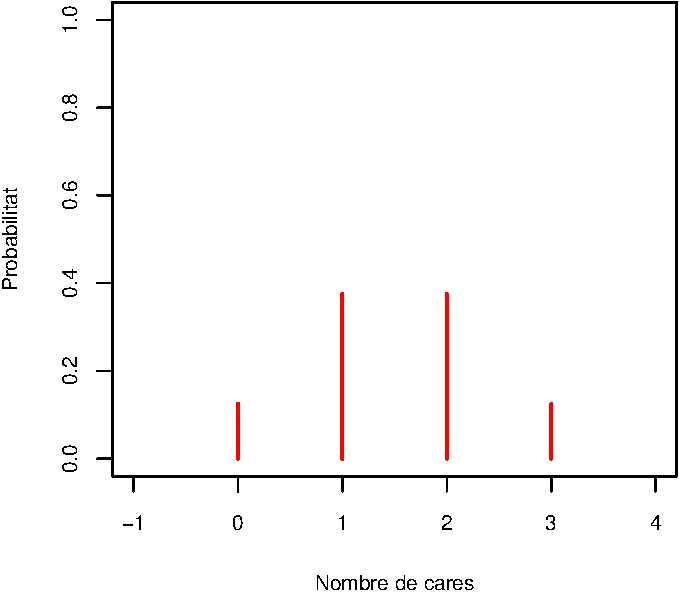
\includegraphics[width=0.6\linewidth]{Bioestadistica-II_files/figure-latex/densicares-1} 

}

\caption{Funció de densitat de la variable aleatòria que compta el nombre de cares en 3 llançaments}\label{fig:densicares}
\end{figure}

\begin{rmdnote}
Si \(X\) és una variable aleatòria discreta, \(P(X\in A)=0\) per a qualsevol subconjunt \(A\) disjunt amb \(D_X\), perquè, per la definició del domini \(D_X\), \(X\) no pot prendre cap valor fora de \(D_X\). Per exemple, quina és la probabilitat de treure entre 2.5 i 2.7 cares en llançar 3 vegades una moneda? 0. I la de treure \(\pi\) cares? 0 un altre cop.
\end{rmdnote}

\begin{itemize}
\item
  Vegem ara la seva \textbf{funció de distribució} \(F_X\). Recordau que \(F_X(x)=P(X\leq x)\) i que la nostra variable només pot prendre els valors 0, 1, 2 i 3.

  \begin{itemize}
  \item
    Si \(x<0\), \(F_X(x)=P(X\leq x)=0\) perquè \(X\) no pot prendre cap valor estrictament negatiu.
  \item
    Si \(0\leq x<1\), \(F_X(x)=P(X\leq x)=P(X=0)=f_X(0)=1/8\), perquè si \(0\leq x<1\), l'únic valor \(\leq x\) que pot prendre \(X\) és el 0.
  \item
    Si \(1\leq x<2\), \(F_X(x)=P(X\leq x)=P(X=0\text{ o }X=1)\) \(=f_X(0)+f_X(1)=4/8=1/2\), perquè si \(1\leq x<2\), els únics valors \(\leq x\) que pot prendre \(X\) són 0 i 1.
  \item
    Si \(2\leq x<3\), \(F_X(x)=P(X\leq x)=P(X=0\text{ o }X=1\text{ o }X=2)\) \(=f_X(0)+f_X(1)+f_X(2)=7/8\), perquè si \(2\leq x<3\), els únics valors \(\leq x\) que pot prendre \(X\) són 0, 1 i 2.
  \item
    Si \(3\leq x\), \(F_X(x)=P(X\leq x)=1\), perquè si \(x\geq 3\), segur que obtenim un nombre de cares \(\leq x\).
  \end{itemize}

  Per tant, la funció \(F_X\) és la funció
  \[
  F_X(x) =\left\{
  \begin{array}{ll}
  0 & \text{ si $x<0$}\\
  1/8 & \text{ si $0\leq x< 1$}\\ 
  4/8 & \text{ si $1\leq x< 2$}\\ 
  7/8 & \text{ si $2\leq x< 3$}\\ 
  1 & \text{ si $3\leq x$}
  \end{array}
  \right.
  \]
  El seu gràfic és el següent:
\end{itemize}

\begin{figure}

{\centering 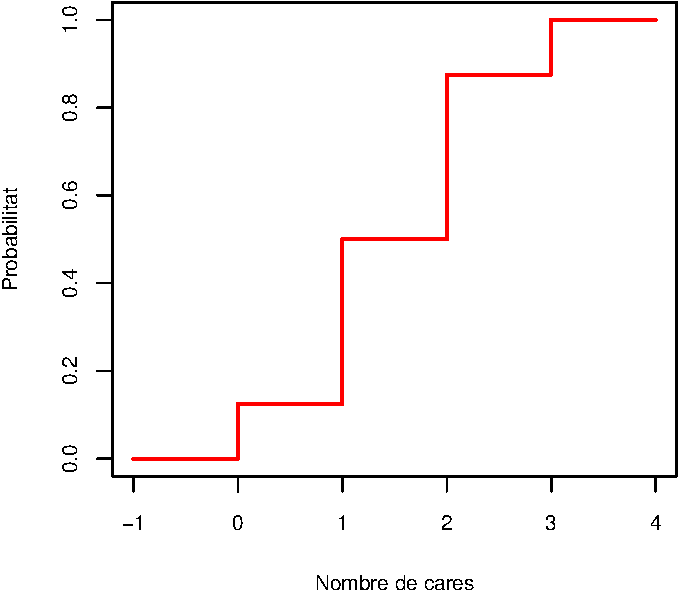
\includegraphics[width=0.6\linewidth]{Bioestadistica-II_files/figure-latex/districares-1} 

}

\caption{Funció de distribució de la variable aleatòria que compta el nombre de cares en 3 llançaments}\label{fig:districares}
\end{figure}

Observau en aquest gràfic que aquesta funció de distribució \(F_X\) és creixent i escalonada. Això és general. Si \(X\) és una variable aleatòria discreta:

\begin{itemize}
\item
  \(F_X\) és una funció \textbf{escalonada}, amb bots en els valors de \(D_X\), que són els únics amb probabilitat estrictament més gran que 0 i per tant els únics que ``sumen'' probabilitat. Més en concret:

  \begin{itemize}
  \item
    Si \(x_0,y_0\in D_X\) i \(x_0<y_0\), llavors \(F_X(x_0)< F_X(y_0)\), perquè, com que \(P(X=y_0)>0\),
    \[
    \begin{array}{rl}
    F_X(x_0)\!\!\!\!\! & =P(X\leq x_0)<P(X\leq x_0)+P(X=y_0)\\
    & =P(X\leq x_0\text{ o }X=y_0)\leq P(X\leq y_0)=F_X(y_0)
    \end{array}
    \]
  \item
    Si \(x_0\in D_X\) i dins \((x_0,x]\) no hi ha cap element de \(D_X\), aleshores \(F_X(x_0)=F_X(x)\), perquè
    \[
    \begin{array}{rl}
    F_X(x)\!\!\!\!\! & =P(X\leq x)=P(X\leq x_0)+P(x_0<X\leq x)\\
    & =P(X\leq x_0)+0= P(X\leq x_0)=F_X(x_0)
    \end{array}
    \]
    perquè, com que \((x_0,x]\cap D_X=\emptyset\), \(P(x_0<X\leq x)=0\).
  \item
    Si \(x_0\in D_X\), \(P(X<x_0)<P(X\leq x_0)\), perquè
    \[
    P(X\leq x_0)=P(X<x_0)+P(X=x_0)>P(X<x_0)
    \]
  \end{itemize}
\item
  \(F_X\) és \textbf{creixent}, perquè si \(x\leq y\), tots els subjectes de \(X\leq x\) també pertanyen a \(X\leq y\), i per tant
  \[
  P(X\leq x)\leq P(X\leq y).
  \]
\item
  Com que els valors que pren \(F_X\) són probabilitats, no poden ser ni més petits que 0 ni més grans que 1.
\end{itemize}

El coneixement de \(f_X\), més les regles del càlcul de probabilitats, permet calcular la probabilitat de qualsevol esdeveniment relacionat amb \(X\):
\[
P(X\in A) =\sum_{x\in A} P(X=x) = \sum_{x\in A} f_X(x)
\]
En particular
\[
F_X(x_0)=P(X\leq x_0)=\sum_{x\leq x_0} f_X(x)
\]

La \textbf{moda} d'una variable aleatòria discreta \(X\) és el valor (o els valors) \(x_0\) tal que \(f_X(x_0)=P(X=x_0)\) és màxim. Per tant, la moda és el valor de \(X\) \textbf{més probable} o \textbf{més freqüent} en la població. Per exemple, per a la nostra variable aleatòria que compta el nombre de cares en 3 llançaments d'una moneda equilibrada, la moda són els valors 1 i 2.

\begin{rmdexercici}
Considerau la variable aleatòria \(X\) ``Llançam una moneda equilibrada tantes vegades com sigui necessari fins que surti una cara per primera vegada, i comptam quantes vegades l'hem haguda de llançar''.

\begin{enumerate}
\def\labelenumi{\arabic{enumi}.}
\tightlist
\item
  Quin és el seu domini?
\item
  Quina és la seva funció de densitat?
\item
  Quina és la seva moda? Què significa?
\item
  Quina és la seva funció de distribució? (Indicació: Calculau primer \(P(X>x)\), tenint en compte que \(X>x\) significa que en els primer \(x\) llançaments ha sortit creu, i per això hem hagut de llançar la moneda més de \(x\) vegades per obtenir una cara.)
\end{enumerate}
\end{rmdexercici}

\hypertarget{esperanuxe7a}{%
\subsection{Esperança}\label{esperanuxe7a}}

Quan prenem una mostra d'una variable aleatòria \(X\) definida sobre una població, podem calcular la mitjana i la desviació típica dels seus valors a fi i efecte d'obtenir una idea de quin és el valor central de la mostra i si els seus valors estan tots molt a prop d'aquest valor central o no. Naturalment, també ens podem preguntar per aquesta mena d'informació per al total de la població: Quin és el ``valor mitjà'' de \(X\) sobre tota la població? Aquesta variable, pren valors molt dispersos, o més aviat els pren concentrats al voltant del seu valor mitjà? La primera pregunta la responem amb la \textbf{mitjana}, o \textbf{esperança}, de \(X\), i la segona amb la seva \textbf{variància} i la seva \textbf{desviació típica}. Comencem amb la primera.

La \textbf{mitjana}, o \textbf{esperança} (o \textbf{valor esperat}, \textbf{valor mitjà}\ldots), d'una variable aleatòria discreta \(X\) amb densitat \(f_X:D_X\to [0,1]\) és
\[
E(X)=\sum_{x\in D_X} x\cdot f_X(x)
\]
Sovint també la indicarem amb \(\mu_X\).

La interpretació natural de \(E(X)\) és que és \textbf{la mitjana dels valors de la variable \(X\) en el total de la població \(\Omega\)}. En efecte, com que \(P(X=x)\) és la proporció de subjectes de \(\Omega\) en els quals \(X\) val \(x\),
\[
E(X)=\sum_{x\in D_X} x\cdot P(X=x)
\]
és la mitjana del valor de \(X\) sobre tots els subjectes de \(\Omega\). Comparau-ho amb l'exemple següent.

\begin{example}
\protect\hypertarget{exm:notes1}{}{\label{exm:notes1} }Si, en una classe, un 10\% dels estudiants han tret un 4 en un examen, un 20\% un 6, un 50\% un 8 i un 20\% un 10, quina ha estat la nota mitjana obtinguda?
\end{example}

Segurament calcularíeu aquesta mitjana de la manera següent:
\[
4\cdot 0.1+6\cdot 0.2+8\cdot 0.5+10\cdot 0.2=7.6
\]
Doncs aquest valor és la \textbf{mitjana} de la variable aleatòria ``Prenc un estudiant d'aquesta classe i mir quina nota ha tret en aquest examen'':
\[
\begin{array}{rl}
E(X)\!\!\!\!\! &=4\cdot P(X=4)+6\cdot P(X=6)+8\cdot P(X=8)+10\cdot P(X=10)\\
& = 4\cdot 0.1+6\cdot 0.2+8\cdot 0.5+10\cdot 0.2=7.6
\end{array}
\]

A banda de la seva interpretació com a ``la mitjana de \(X\) en el total de la població'', \(E(X)\) és també el \textbf{valor esperat de \(X\)}, en el sentit següent:

\begin{quote}
Suposau que prenem a l'atzar una mostra de \(n\) subjectes de la població, mesuram \(X\) sobre ells i calculam la mitjana aritmètica dels \(n\) valors obtinguts. Aleshores, quan la mida \(n\) de la mostra tendeix a \(\infty\), aquesta mitjana aritmètica tendeix a valer \(E(X)\) ``gairebé sempre'', en el sentit que la probabilitat que el seu límit sigui \(E(X)\) és 1.
\end{quote}

És a dir: si mesuràssim \(X\) sobre \textbf{molts} subjectes triats a l'atzar i calculàssim la mitjana dels valors obtinguts, és \textbf{gairebé segur} que obtendríem un valor \textbf{molt proper} a \(E(X)\).

\begin{example}
\protect\hypertarget{exm:unnamed-chunk-15}{}{\label{exm:unnamed-chunk-15} }Seguim amb la variable aleatòria \(X\) ``Llançam una moneda equilibrada 3 vegades i comptam les cares''. El seu valor esperat és
\[
E(X)= 0\cdot \frac{1}{8}+1\cdot \frac{3}{8}+2\cdot \frac{3}{8}+3\cdot \frac{1}{8}=1.5
\]
\end{example}

Això ens diu que:

\begin{itemize}
\item
  La \textbf{mitjana} de \(X\) és 1.5: El valor mitjà de la variable \(X\) sobre tota la població de seqüències de 3 llançaments d'una moneda equilibrada és 1.5.
\item
  L'\textbf{esperança} de \(X\) és 1.5: Si repetíssim moltes vegades l'experiment de llançar la moneda 3 vegades i comptar les cares, la mitjana dels resultats obtinguts donaria, molt probablement, un valor molt pròxim a 1.5. Abreujam això dient que si llançam la moneda 3 vegades, \textbf{esperam treure 1.5 cares}.
\end{itemize}

Més en general, si \(g:\mathbb{R}\to \mathbb{R}\) és una funció, l'\textbf{esperança} de \(g(X)\) és
\[
E(g(X))=\sum_{x\in D_X} g(x)\cdot f_X(x).
\]
Un altre cop, la interpretació natural d'aquest valor és que és la mitjana de \(g(X)\) sobre la població, i també que és el valor ``esperat'' de \(g(X)\) en el sentit anterior.

\begin{example}
\protect\hypertarget{exm:unnamed-chunk-16}{}{\label{exm:unnamed-chunk-16} }Si llançam una moneda equilibrada 3 vegades, comptam les cares i elevam aquest nombre de cares al quadrat, quin valor esperam obtenir?
\end{example}

Serà l'esperança de \(X^2\), on \(X\) és la variable aleatòria ``Llançam una moneda equilibrada 3 vegades i comptam les cares'' (és a dir, aquesta \(X^2\) és la variable aleatòria ``Llançam una moneda equilibrada 3 vegades, comptam les cares i elevam aquest número al quadrat''):

\[
E(X^2)= 0\cdot \frac{1}{8}+1\cdot \frac{3}{8}+2^2\cdot \frac{3}{8}+3^2\cdot \frac{1}{8}=3
\]

\begin{rmdcaution}
Fixau-vos que \(E(X^2) \neq E(X)^2\). Per exemple, en els dos darrers exemples hem vist que si \(X\) és la variable aleatòria que compta el nombre de cares en 3 llançaments d'una moneda equilibrada, \(E(X^2)=3\) però \(E(X)^2=1.5^2=2.25\).

En general, donada una aplicació \(g:\mathbb{R}\to \mathbb{R}\), el més habitual és que \(E(g(X))\neq g(E(X))\).
\end{rmdcaution}

L'esperança de les variables aleatòries discretes té les propietats següents, totes molt raonables si les interpretau en termes del valor mitjà de \(X\) sobre la població:

\begin{itemize}
\item
  Sigui \(b\) una \textbf{variable aleatòria constant}, que sobre tots els individus de la població pren el mateix valor \(b\in \mathbb{R}\). Aleshores, \(E(b)=b\).

  Si en una classe tothom treu un 8 d'un examen, la nota mitjana és un 8, no?
\end{itemize}

\begin{rmdromans}
Sí, ja sabem que parlar de variables constants és un oxímoron, però de vegades una variable aleatòria pren el mateix valor sobre tots els subjectes d'una població. Per exemple ``Prenc un estudiant de Biologia o Bioquímica del curs 2019/20 i compt el seu nombre de cames''.
\end{rmdromans}

\begin{itemize}
\item
  L'esperança és \textbf{lineal}:

  \begin{itemize}
  \item
    Si \(X\) és una variable aleatòria i \(a,b\in \mathbb{R}\), \(E(aX+b)=aE(X)+b\)

    Si en una classe la mitjana d'un examen ha estat un 6 i decidim multiplicar per 1.2 totes les notes i sumar-les 1 punt, la mitjana de la nova nota serà 1.2·6+1=8.2, no?
  \item
    Si \(X,Y\) són dues variables aleatòries, \(E(X+Y)=E(X)+E(Y)\).

    Si en una classe la mitjana de la part de qüestions d'un examen ha estat un 3.5 (sobre 5) i la de la part d'exercicis ha estat un 3 (sobre 5), la nota mitjana de l'examen serà un 3.5+3=6.5, no?
  \item
    Combinant les dues propietats anteriors, si \(X_1,\ldots,X_n\) són variables aleatòries i \(a_1,\ldots,a_n,b\in \mathbb{R}\),
    \[
      E(a_1X_1+\cdots+a_nX_n+b)=a_1E(X_1)+\cdots+a_nE(X_n)+b
      \]
  \end{itemize}
\item
  L'esperança és \textbf{monòtona creixent}: Si \(X\leq Y\) (en el sentit que el valor de \(X\) sobre cada subjecte de la població \(\Omega\) és més petit o igual que el valor de \(Y\) sobre ell), llavors \(E(X)\leq E(Y)\).

  Si tots traieu millor nota de Matemàtiques II que de Matemàtiques I, la nota mitjana de Matemàtiques II serà més gran que la de Matemàtiques I, no?
\end{itemize}

\hypertarget{variuxe0ncia-i-desviaciuxf3-tuxedpica}{%
\subsection{Variància i desviació típica}\label{variuxe0ncia-i-desviaciuxf3-tuxedpica}}

La \textbf{variància} d'una variable aleatòria discreta \(X\) és
\[
\sigma(X)^2 =E((X-\mu_X)^2) =\sum_{x\in D_X} (x-\mu_X)^2\cdot f_X(x)
\]
És a dir, és el valor mitjà del quadrat de la diferència entre \(X\) i la seva mitjana \(\mu_X\). També la indicarem amb \(\sigma_X^2\).

Fixau-vos que es tracta de la traducció ``poblacional'' de la definició de variància per a una mostra, i per tant serveix per mesurar el mateix que aquella: la dispersió dels resultats de \(X\) respecte de la mitjana. Només que ara és per a tota la població, i no per a una mostra.

La identitat següent vos pot ser útil quan hàgiu de calcular variàncies ``a mà''.

\begin{theorem}
\protect\hypertarget{thm:unnamed-chunk-19}{}{\label{thm:unnamed-chunk-19} }\(\sigma(X)^2=E(X^2)-\mu_X^2\).
\end{theorem}

\begin{rmdcorbes}
Operem (i recordau que \(E(X)=\mu_X\))
\[
\begin{array}{rl}
\sigma(X)^2\!\!\!\!\! & =E((X-\mu_X)^2)=E(X^2-2\mu_X\cdot X+\mu_X^2)\\
& = E(X^2)-2\mu_X\cdot E(X)+\mu_X^2\\
& \text{(per la linealitat d'$E$)}\\
& = E(X^2)-2\mu_X^2+\mu_X^2=E(X^2)-\mu_X^2
\end{array}
\]
\end{rmdcorbes}

La \textbf{desviació típica} (o \textbf{desviació estàndard}) d'una variable aleatòria discreta \(X\) és l'arrel quadrada positiva de la seva variància:
\[
\sigma(X)=+\sqrt{\sigma(X)^2}
\]
Com la variància, mesura la dispersió dels valors de \(X\) respecte de la mitjana. També la indicarem amb \(\sigma_X\).

\begin{rmdcaution}
En el context de les variables aleatòries, no hi ha ``variància'' i ``variància mostral'', només ``variància''. El mateix nom us hauria de donar la pista que la ``variància mostral'' està definida només per a mostres.
\end{rmdcaution}

El motiu per introduir la variància \textbf{i} la desviació típica per mesurar la dispersió dels valors de \(X\) és la mateixa que en estadística descriptiva: la variància és més fàcil de manejar (no involucra arrels quadrades) però les seves unitats són les de \(X\) al quadrat, mentre que les unitats de la desviació típica són les de \(X\), i per tant el seu valor és més fàcil d'interpretar.

\begin{example}
\protect\hypertarget{exm:unnamed-chunk-22}{}{\label{exm:unnamed-chunk-22} }Seguim amb la variable aleatòria \(X\) ``Llançam una moneda equilibrada 3 vegades i comptam les cares''. Recordem que \(\mu_X=E(X)=1.5\). Aleshores, la seva variància és:
\end{example}

\[
\begin{array}{rl}
\sigma(X)^2 \!\!\!\!\! & \displaystyle=(0-1.5)^2\cdot \frac{1}{8}+(1-1.5)^2\cdot \frac{3}{8}\\ &\displaystyle\qquad +(2-1.5)^2\cdot \frac{3}{8}+(3-1.5)^2\cdot \frac{1}{8}=0.75
\end{array}
\]
Si recordam que \(E(X^2)=3\), podem veure que
\[
E(X^2)-\mu_X^2=3-1.5^2=0.75=\sigma(X)^2
\]
La seva desviació típica és
\[
\sigma(X) =\sqrt{\sigma(X)^2}=\sqrt{0.75}= 0.866
\]

Vegem algunes propietats de la variància i la desviació típica:

\begin{itemize}
\item
  Si \(b\) és una variable aleatòria constant que sobre tots els individus de la població pren el valor \(b\in \mathbb{R}\), aleshores \(\sigma(b)^2=\sigma(b)=0\).

  Una variable aleatòria constant té zero dispersió.
\item
  \(\sigma(aX+b)^2=a^2\cdot \sigma(X)^2\).
\end{itemize}

\begin{rmdcorbes}
En efecte
\[
\begin{array}{l}
\sigma(aX+b)^2 =E((aX+b)^2)-E(aX+b)^2\\
\quad = E(a^2X^2+2abX+b^2)-(aE(X)+b)^2\\
\quad \text{(per la linealitat de $E$)}\\
\quad = a^2E(X^2)+2abE(X)+b^2-a^2E(X)^2-2abE(X)-b^2\\
\quad \text{(una altre cop, per la linealitat de $E$)}\\
\quad = a^2(E(X^2)-E(X)^2)=a^2\sigma(X)^2
\end{array}
\]
\end{rmdcorbes}

\begin{itemize}
\item
  \(\sigma(aX+b)=|a|\cdot \sigma(X)\) (recordau que la desviació típica és positiva, i \(+\sqrt{a^2}=|a|\)).
\item
  Si \(X,Y\) són variables aleatòries \textbf{independents},
  \[
  \sigma(X+Y)^2=\sigma(X)^2+\sigma(Y)^2
  \]
  i per tant
  \[
  \sigma(X+Y)=\sqrt{\sigma(X)^2+\sigma(Y)^2}
  \]
  Si no són independents, en general aquesta igualtat és falsa. Per posar un exemple extrem,
  \[
  \sigma(X+X)^2=4\sigma(X)^2 \neq \sigma(X)^2+\sigma(X)^2.
  \]
\item
  Més en general, si \(X_1,\ldots,X_n\) són variables aleatòries \textbf{independents} (i, en principi, només en aquest cas) i \(a_1,\ldots,a_n,b\in \mathbb{R}\),
  \[
  \begin{array}{l}
  \sigma(a_1X_1+\cdots+a_nX_n+b)^2=a_1\cdot\sigma(X_1)^2+\cdots+a_n\cdot\sigma(X_n)^2\\
  \sigma(a_1X_1+\cdots+a_nX_n+b)=\sqrt{a_1\cdot\sigma(X_1)^2+\cdots+a_n\cdot\sigma(X_n)^2}
  \end{array}
  \]
\end{itemize}

\hypertarget{quantils}{%
\subsection{Quantils}\label{quantils}}

Sigui \(p\in [0,1]\). El \textbf{quantil d'ordre \(p\)} (o \textbf{\(p\)-quantil}) d'una variable aleatòria discreta \(X\) és el valor \(x_p\in D_X\) tal que \(P(X\leq x_p)\geq p\) però \(P(X< x_p)<p\). És a dir, el valor \(x_p\in D_X\) més petit tal que \(P(X\leq x_p)\geq p\).

Per exemple, que el 0.25-quantil d'una variable aleatòria discreta \(X\) sigui, jo què sé, 8, significa que almenys un 25\% de la població té un valor de \(X\) més petit o igual que 8, però menys d'un 25\% de la població té un valor de \(X\) estrictament més petit que 8. És a dir, 8 és el valor més petit per al qual la probabilitat acumulada arriba al 25\%.

\begin{rmdnote}
Si existeix algun \(x_p\in D_X\) tal que \(P(X\leq x_p)=p\), llavors el \(p\)-quantil és aquest \(x_p\), perquè, per a tot un altre \(x\in D_x\):

\begin{itemize}
\tightlist
\item
  Si \(x<x_p\), \(P(X\leq x)<P(X\leq x_p)=F_X(x_p)=p\) i per tant \(x\) no pot ser el \(p\)-quantil de \(X\).
\item
  Si \(x>x_p\), \(p=P(X\leq x_p)\leq P(X<x)\), i per tant \(x\) tampoc no pot ser el \(p\)-quantil de \(X\).
\end{itemize}
\end{rmdnote}

Com en estadística descriptiva, alguns quantils de variables aleatòries tenen noms propis. Per exemple:

\begin{itemize}
\item
  La \textbf{mediana} de \(X\) és el seu 0.5-quantil.
\item
  El \textbf{primer} i el \textbf{tercer quartils} de \(X\) són els seus \(0.25\)-quantil i \(0.75\)-quantil, respectivament.
\item
  Etc.
\end{itemize}

\begin{example}
\protect\hypertarget{exm:unnamed-chunk-25}{}{\label{exm:unnamed-chunk-25} }Seguim amb la variable aleatòria \(X\) ``Llançam una moneda equilibrada 3 vegades i comptam les cares''. Recordem que la seva funció de distribució és
\end{example}

\[
F_X(x)=\left\{
\begin{array}{ll}
0 & \text{ si $x<0$}\\
0.125 & \text{ si $0\leq x<1$}\\
0.5 & \text{ si $1\leq x<2$}\\
0.875 & \text{ si $2\leq x<3$}\\
1 & \text{ si $3\leq x $}
\end{array}
\right.
\]

\begin{center}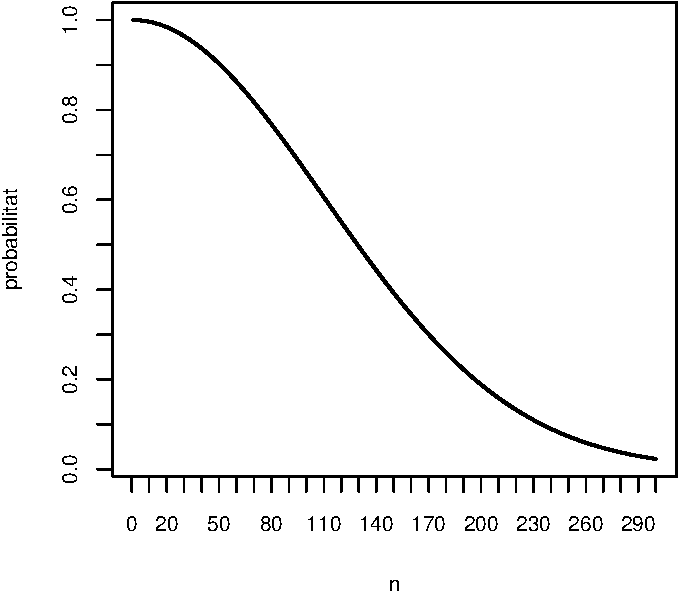
\includegraphics[width=0.6\linewidth]{Bioestadistica-II_files/figure-latex/unnamed-chunk-26-1} \end{center}

Llavors, per exemple:

\begin{itemize}
\item
  El seu 0.125-quantil és 0
\item
  El seu 0.25-quantil és 1
\item
  La seva mediana és 1
\item
  El seu 0.75-quantil és 2
\end{itemize}

\hypertarget{famuxedlies-importants-de-variables-aleatuxf2ries-discretes}{%
\section{Famílies importants de variables aleatòries discretes}\label{famuxedlies-importants-de-variables-aleatuxf2ries-discretes}}

En aquesta secció descriurem tres famílies de variables aleatòries ``distingides'' que heu de conèixer:

\begin{itemize}
\tightlist
\item
  Binomial
\item
  Hipergeomètrica
\item
  Poisson
\end{itemize}

Cadascuna d'aquestes famílies tenen un tipus específic de funció de densitat que depèn d'un o diversos \textbf{paràmetres}.

D'aquestes famílies de variables heu de saber:

\begin{itemize}
\tightlist
\item
  Distingir-les: saber quan una variable aleatòria és d'una família d'aquestes.
\item
  La seva densitat, el seu valor esperat i la seva variància.
\item
  Emprar R per calcular coses amb elles quan sigui necessari.
\end{itemize}

\hypertarget{variables-aleatuxf2ries-binomials}{%
\subsection{Variables aleatòries binomials}\label{variables-aleatuxf2ries-binomials}}

Un \textbf{experiment de Bernoulli} és una acció amb només dos resultats possibles, que identificam amb ``Èxit'' (\(E\)) i ``Fracàs'' (\(F\)), i de la qual, en principi, no podem predir el seu resultat per mor de la influència de l'atzar. Per exemple, llançar un dau cúbic i mirar si ha sortit un 6 (\(E\): treure un 6; \(F\): qualsevol altre resultat).

La \textbf{probabilitat d'èxit} \(p\) d'un experiment de Bernoulli és la probabilitat d'obtenir un èxit \(E\). És a dir, \(P(E)=p\). Naturalment, llavors, \(P(F)=1-p\).

Per exemple, són experiments de Bernoulli

\begin{itemize}
\item
  Llançar una moneda equilibrada i mirar si dóna cara.

  \begin{itemize}
  \tightlist
  \item
    \(E\): donar cara
  \item
    \(p=1/2\)
  \end{itemize}
\item
  Realitzar un test PCR de COVID-19 a una persona i mirar si dóna positiu

  \begin{itemize}
  \item
    \(E\): donar positiu
  \item
    \(p\): la proporció de persones de la població de la qual hem extret el nostre subjecte que donen positiu en el test

    Que no heu de confondre amb la proporció de persones de la població de la qual hem extret el nostre subjecte que tenen la COVID-19.
  \end{itemize}
\end{itemize}

Una \textbf{variable aleatòria de Bernoulli de paràmetre \(p\)} (abreujadament, \(Be(p)\)) és una variable aleatòria \(X\) que consisteix a efectuar un experiment de Bernoulli i donar 1 si s'obté un èxit i 0 si s'obté un fracàs.

Una \textbf{variable aleatòria binomial de paràmetres \(n\) i \(p\)} (abreujadament, \(B(n,p)\)) és una variable aleatòria \(X\) que compta el nombre d'èxits \(E\) en una seqüència de \(n\) repeticions independents d'un mateix experiment de Bernoulli de probabilitat d'èxit \(p\). \textbf{Independents} significa que les \(n\) variables aleatòries de Bernoulli, una per a cada repetició de l'experiment de Bernoulli, són independents; és a dir, que el resultat de cada experiment en la seqüència no depèn dels resultats dels altres.

Direm a \(n\) la \textbf{mida de les mostres} i a \(p\) la \textbf{probabilitat} (\textbf{poblacional}) \textbf{d'èxit}. De vegades també direm d'una variable \(X\) de tipus \(B(n,p)\) que té \textbf{distribució binomial de paràmetres \(n\) i \(p\)}.

Per exemple:

\begin{itemize}
\item
  Una variable de Bernoulli \(Be(p)\) és una variable binomial \(B(1,p)\).
\item
  Llançar una moneda equilibrada 10 vegades i comptar les cares és una variable binomial \(B(10,0.5)\)
\item
  Triar 20 estudiants de la UIB a l'atzar, l'un rere l'altre, permetent repeticions i cada tria independent de les altres, i mirar si al primer semestre han aprovat totes les assignatures o no, és una variable binomial \(B(20,p)\) amb \(p\) la proporció d'estudiants de la UIB que han aprovat totes les assignatures del primer semestre.
\end{itemize}

El tipus més comú de variables binomials que ens interessaran és aquest darrer:

\begin{rmdimportant}
Tenim un subconjunt \(A\) d'una població \(\Omega\) (per exemple, els estudiants de la UIB que han aprovat totes les assignatures del primer semestre). Sigui \(p\) la proporció poblacional d'individus de la població que pertanyen a \(A\), és a dir \(p=P(A)\). Prenem \textbf{mostres aleatòries simples} de mida \(n\) de la població i comptam quants subjectes de la mostra són de \(A\). Aquesta variable aleatòria és \textbf{binomial} \(B(n,p)\).
\end{rmdimportant}

Tenim el resultat següent.

\begin{theorem}
\protect\hypertarget{thm:unnamed-chunk-28}{}{\label{thm:unnamed-chunk-28} }Si \(X\) és una variable \(B(n,p)\):

\begin{itemize}
\item
  El seu domini és \(D_X=\{0,1,\ldots,n\}\)
\item
  La seva funció de densitat és
  \[
  f_X(k)=\left\{\begin{array}{ll}
  \displaystyle\binom{n}{k}p^k(1-p)^{n-k} & \text{ si $k\in D_X$}\\
  0 & \text{ si $k \notin D_X$}
  \end{array}
  \right.
  \]
\item
  El seu valor esperat és \(E(X)=np\)
\item
  La seva variància és \(\sigma(X)^2=np(1-p)\)
\end{itemize}
\end{theorem}

\begin{rmdimportant}
Recordau que:

\begin{itemize}
\item
  El \textbf{factorial} \(m!\) d'un nombre natural \(m\) és \(m!=m(m-1)\cdots 2\cdot 1\) si \(m\geq 1\). Si \(m=0\), es pren \(0!=1\).
\item
  El \textbf{nombre combinatori} \(\binom{n}{k}\) és
  \[
  \binom{n}{k}=\frac{\overbrace{n\cdot (n-1)\cdots (n-k+1)}^k}{k\cdot (k-1)\cdots 2\cdot 1}=\frac{n!}{k!(n-k)!}
  \]
  i ens dóna el nombre de subconjunts de \(k\) elements de \(\{1,\ldots,n\}\).
  \end{rmdimportant}
\end{itemize}

\begin{rmdcorbes}
Suposem que efectuam \(n\) repeticions consecutives i independents d'un experiment de Bernoulli de probabilitat d'èxit \(p\) i comptam el nombre d'èxits \(E\); direm \(X\) a la variable aleatòria resultant. Per seguir la demostració, si no us sentiu molt còmodes amb el raonament amb enes i kas abstractes, anau repetint-lo prenent, per exemple, \(n=4\).

Els possibles resultats són totes les paraules possibles de \(n\) lletres formades per \(E\)'s i \(F\)'s. Com que els experiments successius són independents, la probabilitat de cadascuna d'aquestes paraules és el producte de les probabilitats dels seus resultats individuals. Per tant, si una paraula concreta té \(k\) lletres \(E\) i \(n-k\) lletres \(F\) (s'han obtingut \(k\) èxits i \(n-k\) fracassos), la seva probabilitat és \(p^k(1-p)^{n-k}\), independentment de l'ordre en el qual hàgim obtingut els resultats.

Per calcular la probabilitat d'obtenir una seqüència amb \(k\) èxits, sumarem les probabilitats d'obtenir cadascuna de les seqüències de \(n\) lletres amb \(k\) \(E\)'s. Com que totes tenen la mateixa probabilitat, el resultat serà la probabilitat d'una paraula amb \(k\) \(E\)'s i \(n-k\) \(F\)'s multiplicada pel nombre total de paraules diferents amb \(k\) \(E\)'s i \(n-k\) \(F\)'s.

Quantes paraules hi ha amb \(k\) \(E\)'s i \(n-k\) \(F\)'s? Cada una d'elles queda caracteritzada per les posicions de les \(k\) \(E\)'s, per tant és el nombre de possibles eleccions de conjunts de \(k\) posicions per a les \(E\)'s. Això darrer és el nombre de possibles subconjunts de \(k\) elements (les posicions on hi haurà les \(E\)'s) de \(\{1,\ldots,n\}\), que és el nombre combinatori \(\binom{n}{k}\).
Per tant ja tenim
\[
P(X=k)=\binom{n}{k}p^k(1-p)^{n-k}.
\]

A partir d'aquí, el càlcul del valor esperat i la variància és sumar
\[
\begin{array}{l}
\displaystyle E(X)=\sum_{k=0}^n k\cdot \binom{n}{k}p^k(1-p)^{n-k}\\
\displaystyle \sigma(X)^2=\sum_{k=0}^n k^2\cdot \binom{n}{k}p^k(1-p)^{n-k}-\Big(\sum_{k=0}^n k\cdot \binom{n}{k}p^k(1-p)^{n-k})^2
\end{array}
\]
Us podeu fiar de nosaltres, donen \(np\) i \(np(1-p)\), respectivament.

Si ho pensau, veureu que el valor de \(E(X)\) és l'``esperat''. Vegem, si preneu una mostra aleatòria de \(n\) subjectes d'una població en la qual la proporció de subjectes \(E\) és \(p\), quants subjectes \(E\) ``esperau'' obtenir en la vostra mostra? Doncs una proporció \(p\) de la mostra, és a dir \(p\cdot n\), no?
\end{rmdcorbes}

\begin{rmdnote}
La funció de distribució d'una variable binomial no té una fórmula explícita. Només podem dir que si \(X\) és \(B(n,p)\),
\[
F_X(x)=\sum_{k=0}^{\min\{n,x\}} \binom{n}{k}p^k(1-p)^{n-k}
\]
\end{rmdnote}

\begin{rmdimportant}
És un doi, però, per si de cas, us volem fer observar que si \(X\) és \(B(n,p)\), \(P(X=k)\) no només depèn de \(k\) sinó també dels paràmetres \(n\) i \(p\). Això serà general. Totes les variables aleatòries d'una mateixa família tenen la mateixa funció de densitat, llevat dels valors dels paràmetres, que poden variar d'una variable a una altra.
\end{rmdimportant}

El tipus de teorema anterior és el que fa que ens interessi conèixer algunes famílies distingides freqüents de variables aleatòries. Si, per exemple, reconeixem que una variable aleatòria és binomial i coneixem els seus valors de \(n\) i \(p\) i sabem el teorema anterior, automàticament sabem la seva funció de densitat, i amb ella la seva funció de distribució, el seu valor esperat, la seva variància etc., sense necessitat de deduir tota aquesta informació cada vegada que trobem una variable d'aquestes.

Naturalment, conèixer les propietats de les variables aleatòries binomials només és útil si sabem reconèixer quan estam davant d'una. Fixau-vos que en una variable aleatòria binomial:

\begin{itemize}
\item
  Comptam quantes vegades ocorre un esdeveniment (l'èxit \(E\)) en una seqüència d'intents.
\item
  En cada intent, l'esdeveniment que ens interessa passa o no passa, sense grisos.
\item
  El nombre d'intents és fix, \(n\).
\item
  Cada intent és independent dels altres.
\item
  En cada intent, la probabilitat que passi l'esdeveniment que ens interessa és sempre la mateixa, \(p\).
\end{itemize}

Així, per exemple:

\begin{itemize}
\item
  Una dona té 4 fills. La probabilitat que un fill sigui nina és fixa, 0.51. El sexe de cada fill és independent dels altres. Comptam quantes filles té.

  És una variable binomial \(B(4,0.51)\).
\item
  En una aula hi ha 5 homes i 45 dones. Triam 10 estudiants, un darrere l'altre i sense repetir-los, per fer-los una pregunta. Cada elecció és independent de les altres. Comptam quants homes hem interrogat.

  \textbf{No és una variable binomial}: com que no podem repetir estudiants, en cada ronda la probabilitat de triar un home depèn del sexe dels estudiants triats abans que ell. Per tant la \(p\) no és la mateixa en cada elecció.

  Per exemple, en la primera ronda la probabilitat de triar un home és 5/50=0.1. Ara, si en la primera ronda surt triat un home, la probabilitat que en la segona ronda tornem a triar un home es redueix a 4/49=0.0816, mentre que si en la primera elecció surt una dona, la probabilitat de triar un home en la segona ronda puja a 5/49=0.102.
\item
  En una aula hi ha 5 homes i 45 dones. Triam 10 estudiants, un darrere l'altre però cada estudiant pot ser triat més d'una vegada, per a fer-los una pregunta. Cada elecció és independent de les altres. Comptam quants homes hem interrogat.

  Ara sí que és una variable binomial \(B(10,0.9)\).
\item
  En una aula hi ha 5 homes i 45 dones. Triam estudiants un darrere l'altre i cada estudiant pot ser triat més d'una vegada, per fer-los una pregunta. Cada elecció és independent de les altres. Comptam quants estudiants hem hagut de triar per arribar a interrogar 5 homes.

  No és una variable binomial: no compta el nombre d'èxits en una seqüència d'un nombre fix d'intents, sinó quants intents hem necessitat per arribar a un nombre fix d'èxits.
\item
  En una aula hi ha 5 homes i 45 dones. Llançam una moneda equilibrada: si surt cara triam 10 estudiants i si surt creu en triam 20, per a fer-los una pregunta. Tant en un cas com en l'altre, els triarem un darrere l'altre, cada estudiant podrà ser triat més d'una vegada i cada elecció serà independent de les altres. Comptam quants homes hem interrogat.

  No és una variable binomial: el nombre d'intents no és fix.
\item
  La probabilitat que un dia de novembre plogui és d'un 32\%. Triam una setmana de novembre i comptam quants dies ha plogut.

  No és d'una variable binomial. Encara que \emph{a priori} cada dia tengui la mateixa probabilitat de pluja, que plogui un dia no és independent que plogui l'anterior. Per què fos binomial, hauríem d'haver triat 7 dies de novembre a l'atzar, permetent que sortissin repetits.
\item
  A Espanya hi ha 46,700,000 persones, de les quals un 11.7\% són diabètics. Triam 100 espanyols diferents a l'atzar (de manera independent els uns dels altres) i comptam quants són diabètics.

  No és binomial, però \textbf{pràcticament} sí que ho és, perquè les probabilitats gairebé no varien d'una elecció a la següent. En aquest cas farem la trampa de considerar-la binomial.
\end{itemize}

\begin{example}
\protect\hypertarget{exm:999}{}{\label{exm:999} }Tenim una població de 46,700,000 persones i en volem extreure una mostra aleatòria de 100. Llavors, per exemple, quan ja portau 99 individus escollits, la probabilitat de triar un individu concret dels que queden és
\end{example}

\begin{Shaded}
\begin{Highlighting}[]
\DecValTok{1}\SpecialCharTok{/}\NormalTok{(}\DecValTok{46700000{-}99}\NormalTok{)}
\end{Highlighting}
\end{Shaded}

\begin{verbatim}
## [1] 2.141332e-08
\end{verbatim}

mentre que si permetem repeticions, aquesta probabilitat és

\begin{Shaded}
\begin{Highlighting}[]
\DecValTok{1}\SpecialCharTok{/}\DecValTok{46700000}
\end{Highlighting}
\end{Shaded}

\begin{verbatim}
## [1] 2.141328e-08
\end{verbatim}

Vegem alguns gràfics de la funció densitat de variables aleatòries binomials. Primer, per a \(n=10\) i diferents valors de \(p\).

\begin{center}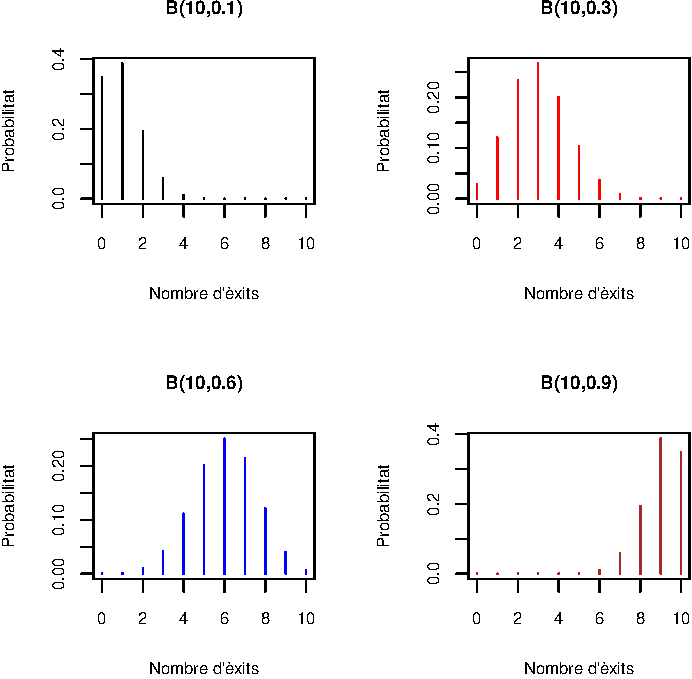
\includegraphics[width=0.9\linewidth]{Bioestadistica-II_files/figure-latex/unnamed-chunk-35-1} \end{center}

Ara per a \(n=100\):

\begin{center}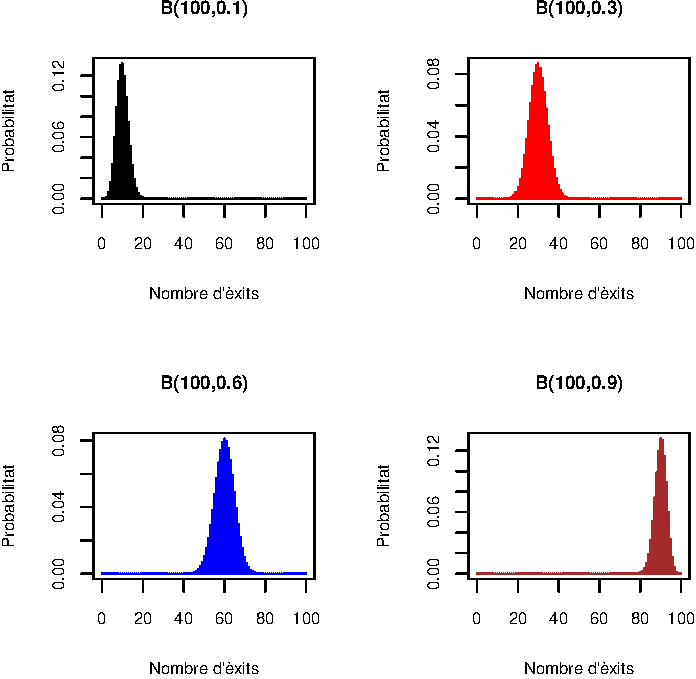
\includegraphics[width=0.9\linewidth]{Bioestadistica-II_files/figure-latex/unnamed-chunk-36-1} \end{center}

Podreu observar que si \(p=0.5\), la funció densitat és simètrica respecte de \(n/2\): com que \(E\) i \(F\) tenen la mateixa probabilitat, 0.5, la probabilitat de treure \(k\) \(E\)'s és la mateixa que la de treure \(k\) \(F\)'s, és a dir, la de treure \(n-k\) \(E\)'s.

\begin{rmdexercici}
Per a agilitar els tests de COVID-19, s'ha proposat l'estratègia següent (anomenada \emph{pooled sample testing} o simplement \emph{pooling}). Unim grups de 10 mostres en una sola mostra i l'analitzam. Si dóna negatiu, serà senyal que totes la mostres originals eren negatives. Declararem llavors negatius els 10 subjectes de les mostres originals. Si dóna positiu, serà perquè almenys una de les mostres originals era positiva. En aquest cas, analitzarem les 10 mostres per separat.

Observau llavors que si les 10 mostres eren negatives, fem un sol test, mentre que si alguna mostra és positiva, en fem 11. Amb l'enfocament tradicional, un test per mostra, sense complicacions, faríem sempre 10 tests.

Suposem que el test té una especificitat i una sensibilitat del 100\%. Sigui \(p\) la prevalença de la COVID-19 en un moment i població donats. Donades 10 mostres preses en aquest moment en aquesta població, quin és el valor esperat de tests que hem de realitzar? Per a \(p\) petita, de l'ordre de l'1\% al 5\%, significaria el \emph{pooling} un estalvi ``esperat'' considerable de tests?
\end{rmdexercici}

\hypertarget{com-efectuar-cuxe0lculs-amb-una-variable-aleatuxf2ria-duna-famuxedlia-donada}{%
\subsubsection*{Com efectuar càlculs amb una variable aleatòria d'una família donada?}\label{com-efectuar-cuxe0lculs-amb-una-variable-aleatuxf2ria-duna-famuxedlia-donada}}
\addcontentsline{toc}{subsubsection}{Com efectuar càlculs amb una variable aleatòria d'una família donada?}

Una possibilitat és usar una aplicació de mòbil o tauleta. La nostra preferida és \emph{Probability distributions}, disponible tant per a Android com per a iOS.

\begin{figure}

{\centering 
\includegraphics[width=0.8\linewidth]{Bioestadistica-II_files/figure-html/appprobdistr} 

}

\caption{L'apli *Probability Distributions*.}\label{fig:unnamed-chunk-38}
\end{figure}

Una altra possibilitat és usar R. R coneix totes la distribucions de variables aleatòries importants; per exemple, per a R la binomial és \texttt{binom}. Aleshores

\begin{itemize}
\item
  Afegint al nom de la distribució el prefix \texttt{d}, tenim la seva funció de \textbf{densitat}: de la binomial serà \texttt{dbinom}.
\item
  Afegint al nom de la distribució el prefix \texttt{p}, tenim la seva funció de \textbf{distribució}: de la binomial, \texttt{pbinom}.
\item
  Afegint al nom de la distribució el prefix \texttt{q}, tenim els seus \textbf{quantils}: per a la binomial, \texttt{qbinom}.
\item
  Afegint al nom de la distribució el prefix \texttt{r}, tenim una funció que produeix \textbf{mostres aleatòries} de nombres amb aquesta distribució de probabilitat: per a la binomial, \texttt{rbinom}.
\end{itemize}

Aquestes funcions s'apliquen a l'argument de la funció i els paràmetres de la variable aleatòria en la seva ordre usual. Per exemple, per a la binomial, s'apliquen a (argument, \(n\), \(p\)). Per a més detalls sobre tot això, consultau la \href{https://aprender-uib.github.io/AprendeR1/chap-distr.html}{lliçó de R sobre el tema}.

Vegem alguns exemples.

\begin{itemize}
\tightlist
\item
  Si llançam 20 vegades un dau cúbic equilibrat, quina és la probabilitat de treure exactament 5 uns? Si diem \(X\) a la variable aleatòria que compta el nombre d'uns en seqüències de 20 llançaments d'un dau equilibrat, es tracta d'una variable binomial \(B(20,1/6)\). Ens demanen \(P(X=5)\), i aquesta probabilitat ens la dóna la funció de densitat de \(X\). És \(f_X(5)\):
\end{itemize}

\begin{Shaded}
\begin{Highlighting}[]
\FunctionTok{dbinom}\NormalTok{(}\DecValTok{5}\NormalTok{,}\DecValTok{20}\NormalTok{,}\DecValTok{1}\SpecialCharTok{/}\DecValTok{6}\NormalTok{)}
\end{Highlighting}
\end{Shaded}

\begin{verbatim}
## [1] 0.1294103
\end{verbatim}

\begin{itemize}
\tightlist
\item
  Si llançam 20 vegades un dau cúbic equilibrat, quina és la probabilitat de treure com a màxim 5 uns? Amb les notacions anteriors, ens demanen \(P(X\leq 5)\), i aquesta probabilitat ens la dóna la funció de distribució de \(X\). És \(F_X(5)\):
\end{itemize}

\begin{Shaded}
\begin{Highlighting}[]
\FunctionTok{pbinom}\NormalTok{(}\DecValTok{5}\NormalTok{,}\DecValTok{20}\NormalTok{,}\DecValTok{1}\SpecialCharTok{/}\DecValTok{6}\NormalTok{)}
\end{Highlighting}
\end{Shaded}

\begin{verbatim}
## [1] 0.8981595
\end{verbatim}

\begin{itemize}
\tightlist
\item
  Si llançam 20 vegades un dau cúbic equilibrat, quina és la probabilitat de treure menys de 5 uns? Amb les notacions anteriors, ens demanen \(P(X< 5)\), és a dir, \(P(X\leq 4)=F_X(4)\):
\end{itemize}

\begin{Shaded}
\begin{Highlighting}[]
\FunctionTok{pbinom}\NormalTok{(}\DecValTok{4}\NormalTok{,}\DecValTok{20}\NormalTok{,}\DecValTok{1}\SpecialCharTok{/}\DecValTok{6}\NormalTok{)}
\end{Highlighting}
\end{Shaded}

\begin{verbatim}
## [1] 0.7687492
\end{verbatim}

\begin{itemize}
\tightlist
\item
  Si llançam 20 vegades un dau cúbic equilibrat, quina és la probabilitat de treure 5 uns o més? Amb les notacions anteriors, ens demanen \(P(X\geq 5)\). Com que el contrari de treure 5 uns o més és treure 4 uns o menys, tenim que \(P(X\geq 5)=1-P(X\leq 4)=1-F_X(4)\):
\end{itemize}

\begin{Shaded}
\begin{Highlighting}[]
\DecValTok{1}\SpecialCharTok{{-}}\FunctionTok{pbinom}\NormalTok{(}\DecValTok{4}\NormalTok{,}\DecValTok{20}\NormalTok{,}\DecValTok{1}\SpecialCharTok{/}\DecValTok{6}\NormalTok{)}
\end{Highlighting}
\end{Shaded}

\begin{verbatim}
## [1] 0.2312508
\end{verbatim}

\begin{itemize}
\tightlist
\item
  Si llançam 20 vegades un dau equilibrat, quin és el més petit nombre \(N\) d'uns per al qual la probabilitat de treure com a màxim \(N\) uns arriba al 25\%? Ens demanen el més petit valor \(N\) tal que \(P(X\leq N)\geq 0.25\), i això per definició és el 0.25-quantil de \(X\):
\end{itemize}

\begin{Shaded}
\begin{Highlighting}[]
\FunctionTok{qbinom}\NormalTok{(}\FloatTok{0.25}\NormalTok{,}\DecValTok{20}\NormalTok{,}\DecValTok{1}\SpecialCharTok{/}\DecValTok{6}\NormalTok{)}
\end{Highlighting}
\end{Shaded}

\begin{verbatim}
## [1] 2
\end{verbatim}

Vegem que en efecte \(N=2\) compleix el demanat: la probabilitat de treure com a màxim 2 uns és

\begin{Shaded}
\begin{Highlighting}[]
\FunctionTok{pbinom}\NormalTok{(}\DecValTok{2}\NormalTok{,}\DecValTok{20}\NormalTok{,}\DecValTok{1}\SpecialCharTok{/}\DecValTok{6}\NormalTok{)}
\end{Highlighting}
\end{Shaded}

\begin{verbatim}
## [1] 0.3286591
\end{verbatim}

i la probabilitat de treure com a màxim 1 un és

\begin{Shaded}
\begin{Highlighting}[]
\FunctionTok{pbinom}\NormalTok{(}\DecValTok{1}\NormalTok{,}\DecValTok{20}\NormalTok{,}\DecValTok{1}\SpecialCharTok{/}\DecValTok{6}\NormalTok{)}
\end{Highlighting}
\end{Shaded}

\begin{verbatim}
## [1] 0.1304203
\end{verbatim}

Veiem per tant que amb 1 un no arribam al 25\% de probabilitat i amb 2 sí.

\begin{itemize}
\tightlist
\item
  Volem simular 50 rondes de llançar 20 vegades un dau equilibrat i comptar els uns, és a dir, volem una mostra aleatòria de mida 50 de la nostra variable \(X\):
\end{itemize}

\begin{Shaded}
\begin{Highlighting}[]
\FunctionTok{rbinom}\NormalTok{(}\DecValTok{50}\NormalTok{,}\DecValTok{20}\NormalTok{,}\DecValTok{1}\SpecialCharTok{/}\DecValTok{6}\NormalTok{)}
\end{Highlighting}
\end{Shaded}

\begin{verbatim}
##  [1]  5  3  1  3  5  5  3  5  4  5  1  2  4  4  5  6  1  2  3  2  5  3  4  3  4
## [26]  3  4  5  4  5  5  1  1  1  3  1  3  3  4  4  3  4  4  4  7  6  1  5 10  4
\end{verbatim}

Cada vegada que repetim aquesta instrucció segurament obtendrem una mostra aleatòria nova:

\begin{Shaded}
\begin{Highlighting}[]
\FunctionTok{rbinom}\NormalTok{(}\DecValTok{50}\NormalTok{,}\DecValTok{20}\NormalTok{,}\DecValTok{1}\SpecialCharTok{/}\DecValTok{6}\NormalTok{)}
\end{Highlighting}
\end{Shaded}

\begin{verbatim}
##  [1] 3 4 3 8 3 5 4 4 0 4 4 5 3 1 4 0 4 4 3 4 2 1 2 1 3 3 0 4 1 2 5 2 4 2 4 6 4 5
## [39] 4 2 2 4 6 5 6 4 4 1 5 3
\end{verbatim}

\begin{Shaded}
\begin{Highlighting}[]
\FunctionTok{rbinom}\NormalTok{(}\DecValTok{50}\NormalTok{,}\DecValTok{20}\NormalTok{,}\DecValTok{1}\SpecialCharTok{/}\DecValTok{6}\NormalTok{)}
\end{Highlighting}
\end{Shaded}

\begin{verbatim}
##  [1] 4 1 2 1 5 6 2 2 7 3 3 0 1 4 2 1 2 6 3 3 1 3 4 5 4 5 2 2 4 2 2 4 2 4 4 6 7 8
## [39] 6 2 3 5 3 2 1 4 3 2 4 2
\end{verbatim}

\begin{Shaded}
\begin{Highlighting}[]
\FunctionTok{rbinom}\NormalTok{(}\DecValTok{50}\NormalTok{,}\DecValTok{20}\NormalTok{,}\DecValTok{1}\SpecialCharTok{/}\DecValTok{6}\NormalTok{)}
\end{Highlighting}
\end{Shaded}

\begin{verbatim}
##  [1] 3 4 6 4 5 3 3 5 3 3 2 1 5 7 3 6 5 1 1 3 5 1 6 4 3 5 2 7 4 5 3 1 2 3 4 1 3 3
## [39] 2 3 6 2 1 2 2 3 2 3 2 4
\end{verbatim}

\hypertarget{variables-aleatuxf2ries-hipergeomuxe8triques}{%
\subsection{Variables aleatòries hipergeomètriques}\label{variables-aleatuxf2ries-hipergeomuxe8triques}}

Recordau que el paradigma de variable aleatòria binomial és: tenc una població amb una proporció \(p\) de subjectes que satisfan una condició \(E\), prenc una mostra aleatòria simple de mida \(n\) i compt el nombre de subjectes \(E\) en la meva mostra. Si canviam ``mostra aleatòria simple'' per ``mostra aleatòria sense reposició'', la distribució de la variable aleatòria que obtenim és una altra: és \textbf{hipergeomètrica}.

Una variable aleatòria és \textbf{hipergeomètrica} (o té distribució hipergeomètrica) \textbf{de paràmetres \(N\), \(M\) i \(n\)} (abreujadament, \(H(N,M,n)\)) quan es pot identificar amb el procés següent: Tenim una població formada per \(N\) subjectes que satisfan una condició \(E\) i \(M\) subjectes que no la satisfan (per tant, en total, \(N+M\) subjectes en la població), prenem una mostra aleatòria \textbf{sense reposició} de mida \(n\) i comptam el nombre de subjectes \(E\) en aquesta mostra.

Direm a \(N\) el \textbf{nombre poblacional d'èxits}, a \(M\) el \textbf{nombre poblacional de fracassos} i a \(n\) la \textbf{mida de les mostres}. Fixau-vos llavors que \(N+M\) és la \textbf{mida total de la població} i que \(N/(N+M)\) és la \textbf{probabilitat poblacional d'èxit} (la fracció de subjectes que satisfan \(E\) en el total de la població). Amb R, igual que la distribució binomial era \texttt{binom}, la distribució hipergeomètrica és \texttt{hyper}.

Tenim el resultat següent:

\begin{theorem}
\protect\hypertarget{thm:unnamed-chunk-48}{}{\label{thm:unnamed-chunk-48} }Si \(X\) és una variable \(H(N,M,n)\):

\begin{itemize}
\item
  El seu domini és \(D_X=\{0,1,\ldots,\text{min}(N,n)\}\)
\item
  La seva funció de densitat és
  \[
  f_X(k)=\left\{\begin{array}{ll}
  \displaystyle\dfrac{\binom{N}{k}\cdot \binom{M}{n-k}}{\binom{N+M}{n}} & \text{ si $k\in D_X$}\\
  0 & \text{ si $k\notin D_X$}
  \end{array}
  \right.
  \]
\item
  El seu valor esperat és \(E(X)=\dfrac{nN}{N+M}\)
\item
  La seva variància és \(\sigma(X)^2=\dfrac{nNM(N+M-n)}{(N+M)^2(N+M-1)}\)
\end{itemize}
\end{theorem}

Fixau-vos que si diem \(p\) a la probabilitat poblacional d'èxit, \(p=N/(N+M)\), llavors
\[
E(X)=np.
\]
És la mateixa fórmula que per a les variables binomials \(B(n,p)\) (i si ho pensau una estona veureu que, un altre cop i pel mateix argument, és el que toca). D'altra banda, si diem \(\mathbf{P}\) a la mida total de la població, \(\mathbf{P}=N+M\), llavors
\[
\sigma(X)^2=n\cdot\dfrac{N}{N+M}\cdot\dfrac{M}{N+M}\cdot\frac{N+M-n}{N+M-1}=np(1-p)\cdot\dfrac{\mathbf{P}-n}{\mathbf{P}-1}
\]
que és la variància d'una variable \(B(n,p)\) multiplicada per un factor de correcció a causa del fet que ara prenem mostres sense repetició i la variància és més petita que si les prenem amb repetició. A aquest factor \((\mathbf{P}-n)/(\mathbf{P}-1)\) se'n diu \textbf{factor de població finita}.

Fixau-vos que si \(\mathbf{P}\) és moltíssim més gran que \(n\), tendrem que \(\mathbf{P}-n\approx \mathbf{P}-1\) i per tant \((\mathbf{P}-n)/(\mathbf{P}-1)\approx 1\) i la variància de la hipergeomètrica serà aproximadament la de la binomial. Això és consistent amb el que ja hem comentat: si la població és molt més gran que la mostra, prendre les mostres amb o sense reposició no afecta massa a les mostres obtingudes, per la qual cosa la distribució de probabilitat ha de ser molt semblant.
Recordau els exemples següents:

\begin{itemize}
\item
  A Espanya hi ha 46,700,000 persones, de les quals un 11.7\% són diabètics. Triam 100 espanyols i comptam quants són diabètics.

  Aquesta variable és, en realitat, hipergeomètrica amb \(N=0.117\cdot 46700000=5463900\), \(M=46700000-N=41236100\) i \(n=100\), però en la pràctica la consideram binomial \(B(100,0.117)\). El factor de població finita és
  \[
  \frac{46700000-100}{46700000-1}=0.9999979
  \]
  Pràcticament 1. En canvi:
\item
  En una aula hi ha 5 homes i 45 dones. Triam 10 estudiants, un darrere l'altre i sense repetir-los, per fer-los una pregunta. Cada elecció és independent de les altres. Comptam quants homes hem interrogat.

  Aquesta variable és hipergeomètrica \(H(5,45,10)\). El factor de població finita en aquesta cas no és aproximadament 1: dóna
  \[
  \frac{50-10}{50-1}=0.8163
  \]
  No és correcte aproximar-la per una binomial \(B(10,0.1)\).
\end{itemize}

El gràfic següent compara la funció de densitat d'una variable \(B(10,0.1)\) amb les de variables hipergeomètriques \(H(5,45,10)\), \(H(50,450,10)\) i \(H(5000,45000,10)\) perquè vegeu com a mesura que la mida de la població creix (mantenint constant la proporció poblacional d'èxits), la distribució hipergeomètrica s'aproxima a la binomial.

\begin{center}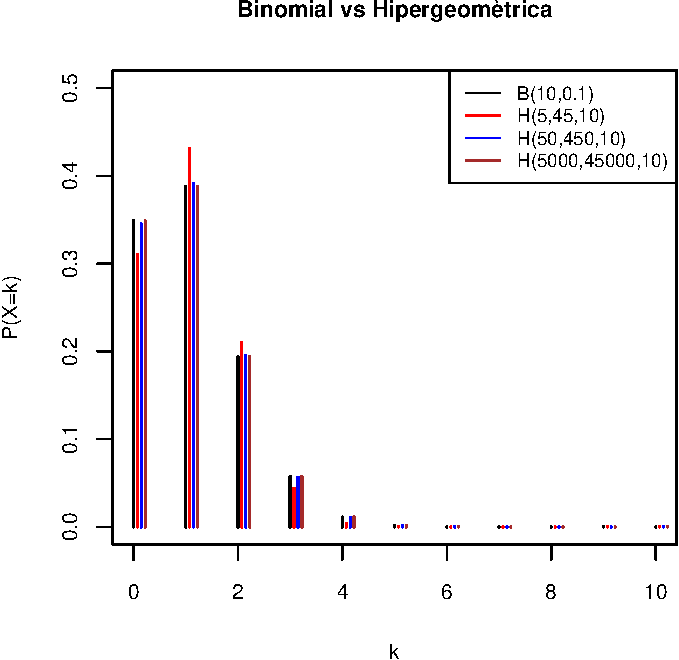
\includegraphics[width=0.5\linewidth]{Bioestadistica-II_files/figure-latex/unnamed-chunk-49-1} \end{center}

\hypertarget{variables-aleatuxf2ries-de-poisson}{%
\subsection{Variables aleatòries de Poisson}\label{variables-aleatuxf2ries-de-poisson}}

Una variable aleatòria \(X\) és \textbf{de Poisson} (o té distribució de Poisson) \textbf{de paràmetre \(\lambda>0\)} (abreujadament, \(Po(\lambda)\)) quan:

\begin{itemize}
\item
  El seu \textbf{domini} és \(D_X=\mathbb{N}\), el conjunt de tots els nombres naturals (és a dir, pot prendre com a valor qualsevol nombre natural).
\item
  La seva \textbf{funció de densitat} és
  \[
  f_X(k)=\left\{\begin{array}{ll}
  e^{-\lambda}\cdot \dfrac{\lambda^k}{k!} & \text{ si $k\in \mathbb{N}$}\\
  0 & \text{ si $k
  \notin \mathbb{N}$}
  \end{array}
  \right.
  \]
\end{itemize}

Per a R, la distribució de Poisson és \texttt{pois}.

\begin{theorem}
\protect\hypertarget{thm:unnamed-chunk-50}{}{\label{thm:unnamed-chunk-50} }Si \(X\) és una variable \(Po(\lambda)\), aleshores \(E(X)= \sigma(X)^2= \lambda\).
\end{theorem}

És a dir, el paràmetre \(\lambda\) d'una variable de Poisson és el seu valor esperat, i coincideix amb la seva variància.

Us deveu estar demanant: per a què ens serveix definir una variable de Poisson mitjançant la seva densitat, si el que ens interessa és poder classificar una variable com a Poisson (o binomial, o hipergeomètrica etc.) per a així saber ``gratis'' la seva densitat? La resposta és que la família de Poisson inclou un tipus de variables aleatòries molt freqüent

Suposem que tenim un tipus d'objectes que poden donar-se en una regió contínua de temps o espai. Per exemple, defuncions de persones per una determinada malaltia en el decurs del temps, exemplars d'una espècie de planta en un terreny, o nombres de bacteris en bocins d'una superfície.

Suposem a més que les aparicions d'aquests objectes satisfan les propietats següents (per simplificar el llenguatge, hi suposarem que observam aparicions d'aquests objectes en el temps; si es tracta d'una variable que compta objectes en regions de l'espai, canviau-hi ``instant'' per ``punt''):

\begin{itemize}
\item
  Les aparicions dels objectes són \textbf{aleatòries}: en cada instant, un objecte es dóna, o no, a l'atzar, amb una probabilitat fixa i constant.
\item
  Les aparicions dels objectes són \textbf{independents}: que es doni un objecte en un instant concret, no depèn per a res que s'hagi donat o no un objecte en un altre instant.
\item
  Les aparicions dels objectes no són \textbf{simultànies}: és pràcticament impossible que dos objectes d'aquests es donin en el mateix instant exacte, mesurat amb precisió infinita.
\end{itemize}

\begin{rmdimportant}
En aquesta situació, la variable \(X_t\) que pren un interval de temps de durada \(t\) i compta el nombre d'objectes que es donen en ell és de Poisson \(Po(\lambda_t)\), amb \(\lambda_t\) el nombre esperat d'objectes en aquest interval de temps (és a dir, el nombre mitjà d'objectes en intervals de temps d'aquesta mida).
\end{rmdimportant}

Per exemple, quan el que compten ocorre a l'atzar, són variables de Poisson:

\begin{itemize}
\item
  El nombre de malalts admesos en urgències en un dia (o en 12 hores, o en una setmana\ldots)
\item
  El nombre de defuncions per una malaltia concreta en un dia (o en una setmana, o en un any\ldots)
\item
  El nombre de bacteris en un quadrat d'1 cm de costat (o d'1 m de costat\ldots)
\end{itemize}

Fixau-vos que aquest tipus de coneixement ens serveix per a dues coses:

\begin{itemize}
\item
  Si sabem que aquestes variables són de Poisson, coneixem la seva densitat i per tant podem calcular el que volguem per a elles.
\item
  Si les dades que observam tocarien seguir una distribució de Poisson però sembla que no (per exemple, perquè la seva variància sigui molt diferent de la seva mitjana, tan diferent que sigui difícil de creure que la mitjana i la variància poblacionals siguin iguals), llavors és senyal que qualque cosa ``estranya'' està passant que desbarata la seva aparició.
\end{itemize}

\begin{example}
\protect\hypertarget{exm:unnamed-chunk-52}{}{\label{exm:unnamed-chunk-52} }Observau la diferència entre les dues variables següents:

\begin{itemize}
\item
  Nombres mensuals de defuncions per un tipus de càncer en un país. El moment exacte de les defuncions es produeix a l'atzar, segurament mai no es donen dues defuncions exactament en el mateix instant, si els poguéssim mesurar amb precisió infinita, i les defuncions es produeixen de manera independent. És de Poisson.
\item
  Nombres mensuals de defuncions per una malatia infecciosa en un país. Un altre cop, el moment exacte de les defuncions es produeix a l'atzar i segurament mai no es donen dues defuncions exactament en el mateix instant, si els poguéssim mesurar amb precisió infinita. Però les infeccions no són independents, precisament perquè es tracta d'una malaltia infecciosa, i per tant les defuncions tampoc: com ens hem cansat d'observar amb la COVID-19, en un mateix \emph{cluster} de la malaltia es poden produir diverses morts associades. No és de Poisson.
\end{itemize}
\end{example}

\begin{rmdnote}
Com que les aparicions dels objectes que compta una variable de Poisson són aleatòries i independents, el nombre mitjà d'objectes és lineal en la mida de la regió. És a dir, per exemple, en un interval de dos dies esperam veure el doble d'objectes que en un dia. O per exemple, si es diagnostiquen de mitjana 32,240 casos de càncer de còlon anuals a Espanya (i segueixen una llei de Poisson), esperam que de mitjana es diagnostiquin 32240/52=620 casos setmanals.
\end{rmdnote}

\hypertarget{variables-aleatuxf2ries-contuxednues}{%
\section{Variables aleatòries contínues}\label{variables-aleatuxf2ries-contuxednues}}

Una variable aleatòria és \textbf{contínua} quan els seus possibles valors són dades quantitatives contínues. Per exemple:

\begin{itemize}
\tightlist
\item
  Pes
\item
  Nivell de colesterol en sang
\item
  Diàmetre d'un tumor
\end{itemize}

En aquest curs ens restringirem a variables aleatòries contínues \(X: \Omega\to \mathbb{R}\) que satisfan la propietat extra següent: la seva \textbf{funció de distribució}
\[
\begin{array}{rcl}
F_X: \mathbb{R} & \to & [0,1]\\
x &\mapsto &P(X\leq x)
\end{array}
\]
és contínua. Totes les variables aleatòries contínues que us puguin interessar en algun moment satisfan aquesta propietat, així que no perdem res imposant-la.

Si \(X\) és una variable aleatòria contínua amb funció de distribució contínua, \textbf{la probabilitat que prengui cada valor concret és 0}:
\[
P(X=a)=0 \text{ per a tot $a \in \mathbb{R}$}.
\]

\begin{rmdcorbes}
Per si passa per aquí qualcú que en necessiti una demostració:
\[
\begin{array}{l}
\displaystyle P(X=a) = P(X\leq a)-P(X<a)=P(X\leq a)-P\Big(\bigcup_{n\geq 1} \Big(X\leq a-\frac{1}{n}\Big)\Big)\\
\displaystyle \qquad= P(X\leq a)-\lim_{n\geq 1}P\Big(X\leq a-\frac{1}{n}\Big)\\
\displaystyle \qquad= F_X(a)-\lim_{n\geq 1}F_X\Big(a-\frac{1}{n}\Big)=0
\end{array}
\]
perquè \(F_X\) és contínua.
\end{rmdcorbes}

En particular, per a una variable aleatòria contínua:

\begin{quote}
\textbf{Probabilitat 0 no significa impossible.}
\end{quote}

Cada valor de \(X\) té probabilitat 0, però si prenem un subjecte de la població, \(X\) tendrà qualque valor sobre ell, no? Per tant, aquest valor de \(X\) és possible, malgrat tengui probabilitat 0.

De \(P(X=a)=0\) es dedueix que la probabilitat d'un esdeveniment definit amb una desigualtat és exactament la mateixa que la de l'esdeveniment corresponent definit amb una desigualtat estricta. En particular, contràriament al que passava a les variables aleatòries discretes, per a una variable aleatòria contínua \textbf{sempre} tenim que
\[
P(X\leq a)=P(X<a)
\]
perquè
\[
P(X\leq a)=P(X<a)+P(X=a)=P(X<a)+0=P(X<a).
\]

Més exemples:

\begin{itemize}
\tightlist
\item
  \(P(X\geq a)=P(X> a)+P(X=a)=P(X> a)\)
\item
  \(P(a \leq X\leq b)=P(a<X <b)+P(X=a)+P(X=b)\) \(=P(a<X <b)\)
\end{itemize}

\hypertarget{densitat-i-distribuciuxf3-1}{%
\subsection{Densitat i distribució}\label{densitat-i-distribuciuxf3-1}}

Sigui \(X\) una variable aleatòria contínua. Com ja hem dit, la seva \textbf{funció de distribució} \(F_X\) torna a ser
\[
x\mapsto F_X(x)=P(X\leq x)
\]

Però com que ara tenim que \(P(X=x)=0\) per a tot \(x\in \mathbb{R}\), no podem definir la funció de densitat de \(X\) com a \(f_X(x)=P(X=x)\). Què podem fer?

Recordau que, a les variables aleatòries discretes,
\[
F_X(a)=\sum_{x\leq a} f_X(x)
\]

En el context de matemàtiques ``contínues'', la suma \(\sum\) es tradueix en una integral \(\int\). Definim aleshores la \textbf{funció de densitat} d'una variable aleatòria contínua \(X\) com la funció \(f_X:\mathbb{R}\to \mathbb{R}\) tal que:

\begin{itemize}
\item
  \(f_X(x)\geq 0\), per a tot \(x\in \mathbb{R}\)
\item
  \(\displaystyle F_X(a)=\int_{-\infty}^a f_{X}(x)\, dx\) per a tot \(a \in \mathbb{R}\).
\end{itemize}

\begin{center}
\includegraphics[width=0.2\linewidth]{Bioestadistica-II_files/figure-html/dontpanic} \end{center}

Recordau que la integral té una interpretació senzilla en termes d'àrees. En concret, donats \(a \in \mathbb{R}\) i una funció \(f(x)\), la integral
\[
\int_{-\infty}^a f(x)\, dx
\]
és igual a l'àrea de la regió compresa entre la corba \(y=f(x)\) i l'eix d'abscisses \(y=0\) a l'esquerra de la recta vertical \(x=a\). Per tant, la funció de densitat \(f_X\) de \(X\) és la funció positiva tal que, per a tot \(a\in \mathbb{R}\), \(F_X(a)\) és igual a \textbf{l'àrea sota la corba} \(y=f_X(x)\) (és a dir, entre aquesta corba i l'eix d'abscisses) a l'esquerra de \(x=a\).

\begin{center}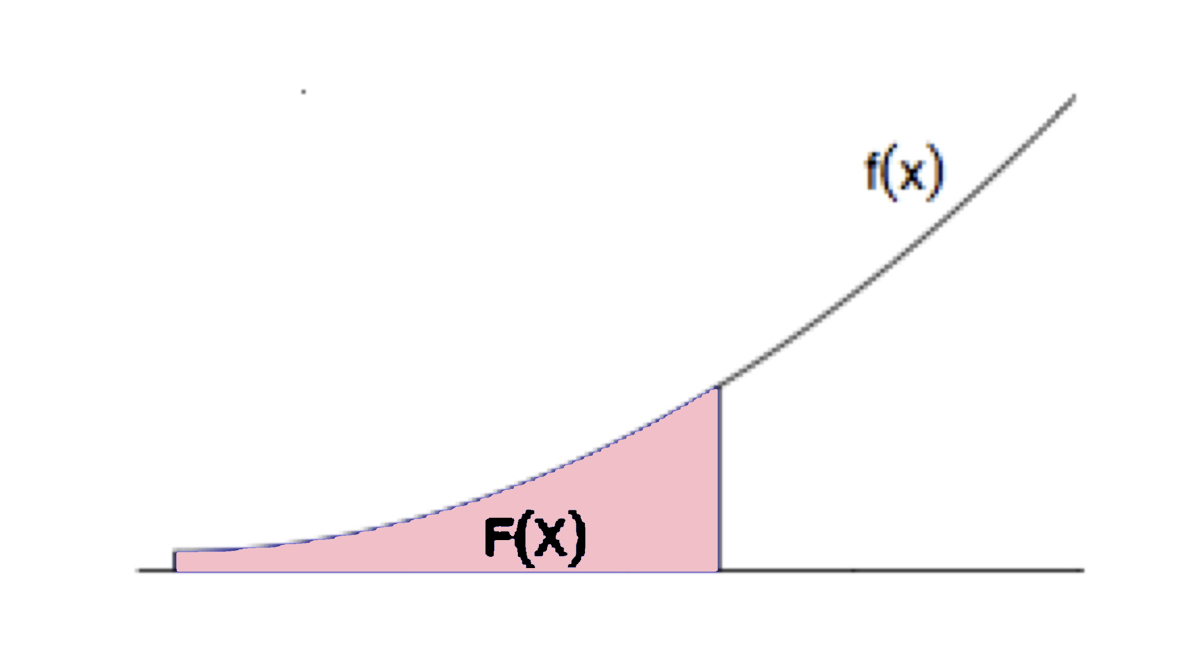
\includegraphics[width=0.6\linewidth]{Bioestadistica-II_files/figure-html/graficadensidad3} \end{center}

Quina és la idea intuïtiva que hi ha al darrere d'aquesta definició de densitat? Suposau que dibuixam histogrames de freqüències relatives dels valors de \(X\) sobre tota la població. Recordau que, en un histograma de freqüències relatives, la freqüència relativa de cada classe (ara la \textbf{probabilitat}, ja que parlam de tota la població) és l'àrea de la seva barra, és a dir, l'amplada de la classe per l'alçada de la barra. I que diem a aquesta alçada la \textbf{densitat} de la classe (i per tant, qualque cosa tendrà a veure amb la densitat de \(X\), no trobau?).

Si dibuixam els histogrames de \(X\) prenent classes cada vegada més estretes, els seus polígons de freqüències tendeixen a dibuixar una corba, que hem acolorit en vermell en el darrer histograma de la seqüència següent:

\begin{center}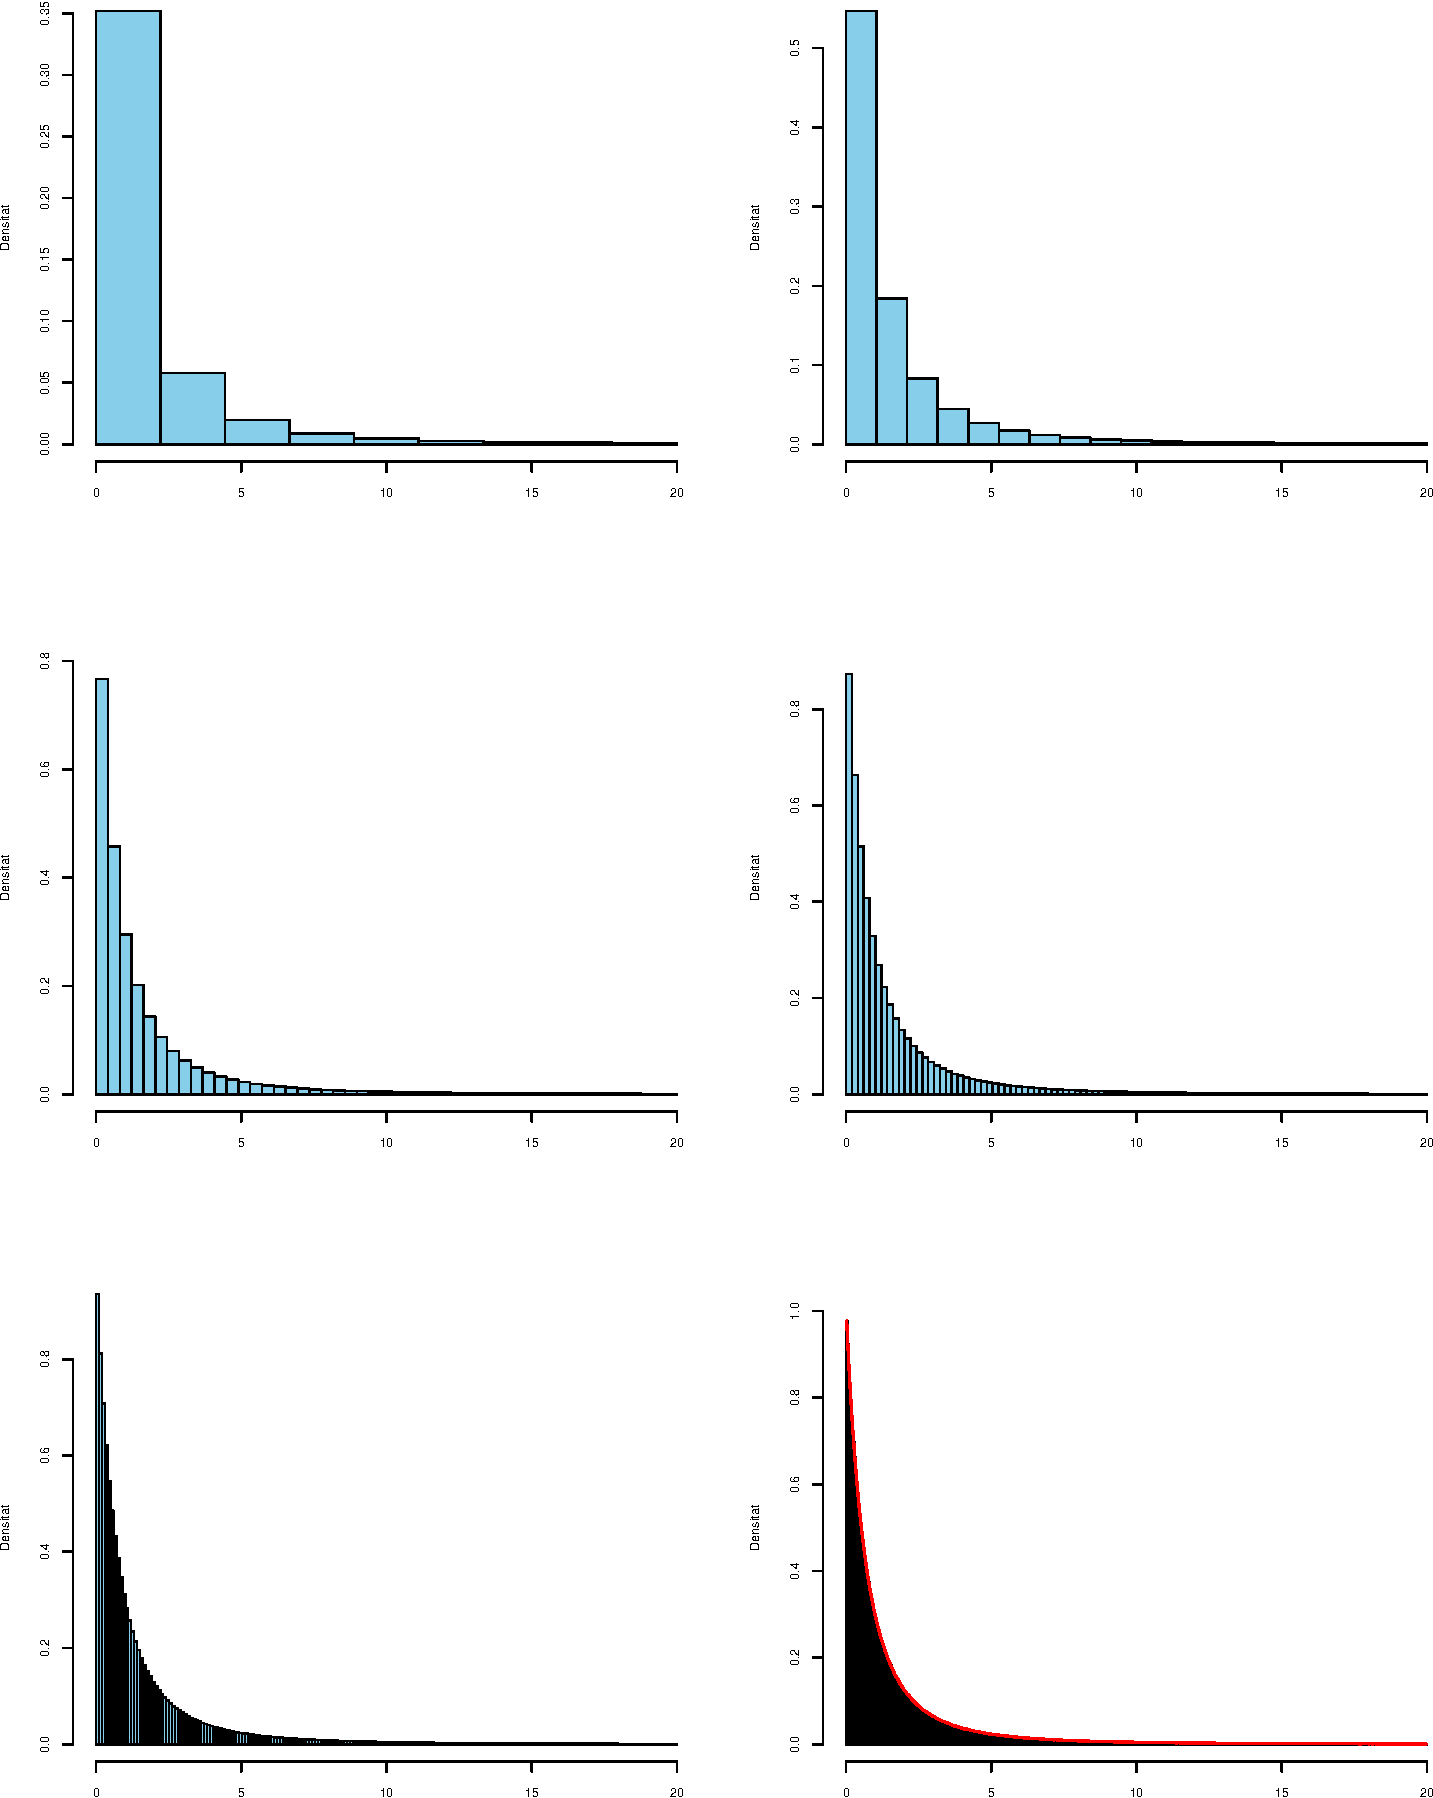
\includegraphics[width=1\linewidth]{Bioestadistica-II_files/figure-latex/unnamed-chunk-57-1} \end{center}

Quan l'amplada de les classes tendeix a 0, obtenim una corba que és el límit d'aquests polígons de freqüències:

\begin{center}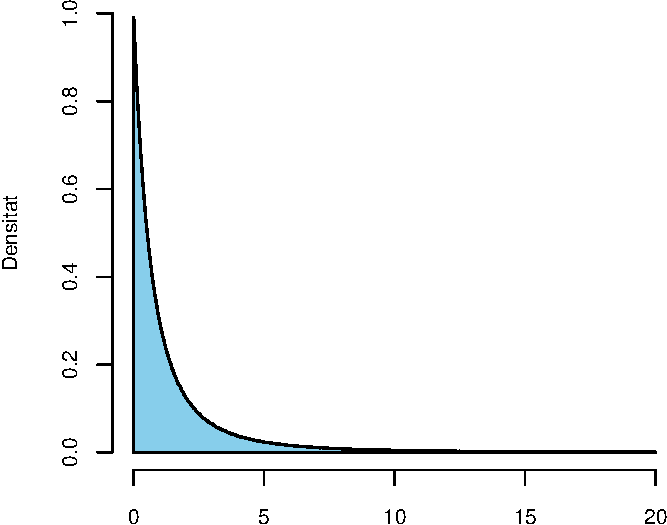
\includegraphics[width=0.5\linewidth]{Bioestadistica-II_files/figure-latex/unnamed-chunk-58-1} \end{center}

Aquesta corba és precisament \(y=f_X(x)\).

\begin{rmdimportant}
La \textbf{funció de densitat} \(f_X\) d'una variable aleatòria contínua \(X\) és la funció límit dels polígons de freqüències d'histogrames de \(X\) quan l'amplada de les classes tendeix a 0.
\end{rmdimportant}

Vegem algunes propietats que es dedueixen del fet que \(F_X(a)=P(X\leq a)\) sigui igual a \textbf{l'àrea sota la corba} \(y=f_X(x)\) a l'esquerra de \(x=a\):

\begin{itemize}
\item
  Com que \(P(X<\infty)=P(\Omega)=1\), \textbf{l'àrea total sota la curva \(y=f_X(x)\) és 1.}
\item
  \(P(a\leq X\leq b)=P(X\leq b)-P(X<a)\) és l'àrea sota la corba \(y=f_X(x)\) a l'esquerra de \(x=b\) \textbf{menys} l'àrea sota la corba \(y=f_X(x)\) a l'esquerra de \(x=a\). Per tant, \(P(a\leq X\leq b)\) és igual a \textbf{l'àrea sota la corba \(y=f_X(x)\) entre \(x=a\) i \(x=b\).}
\end{itemize}

\begin{center}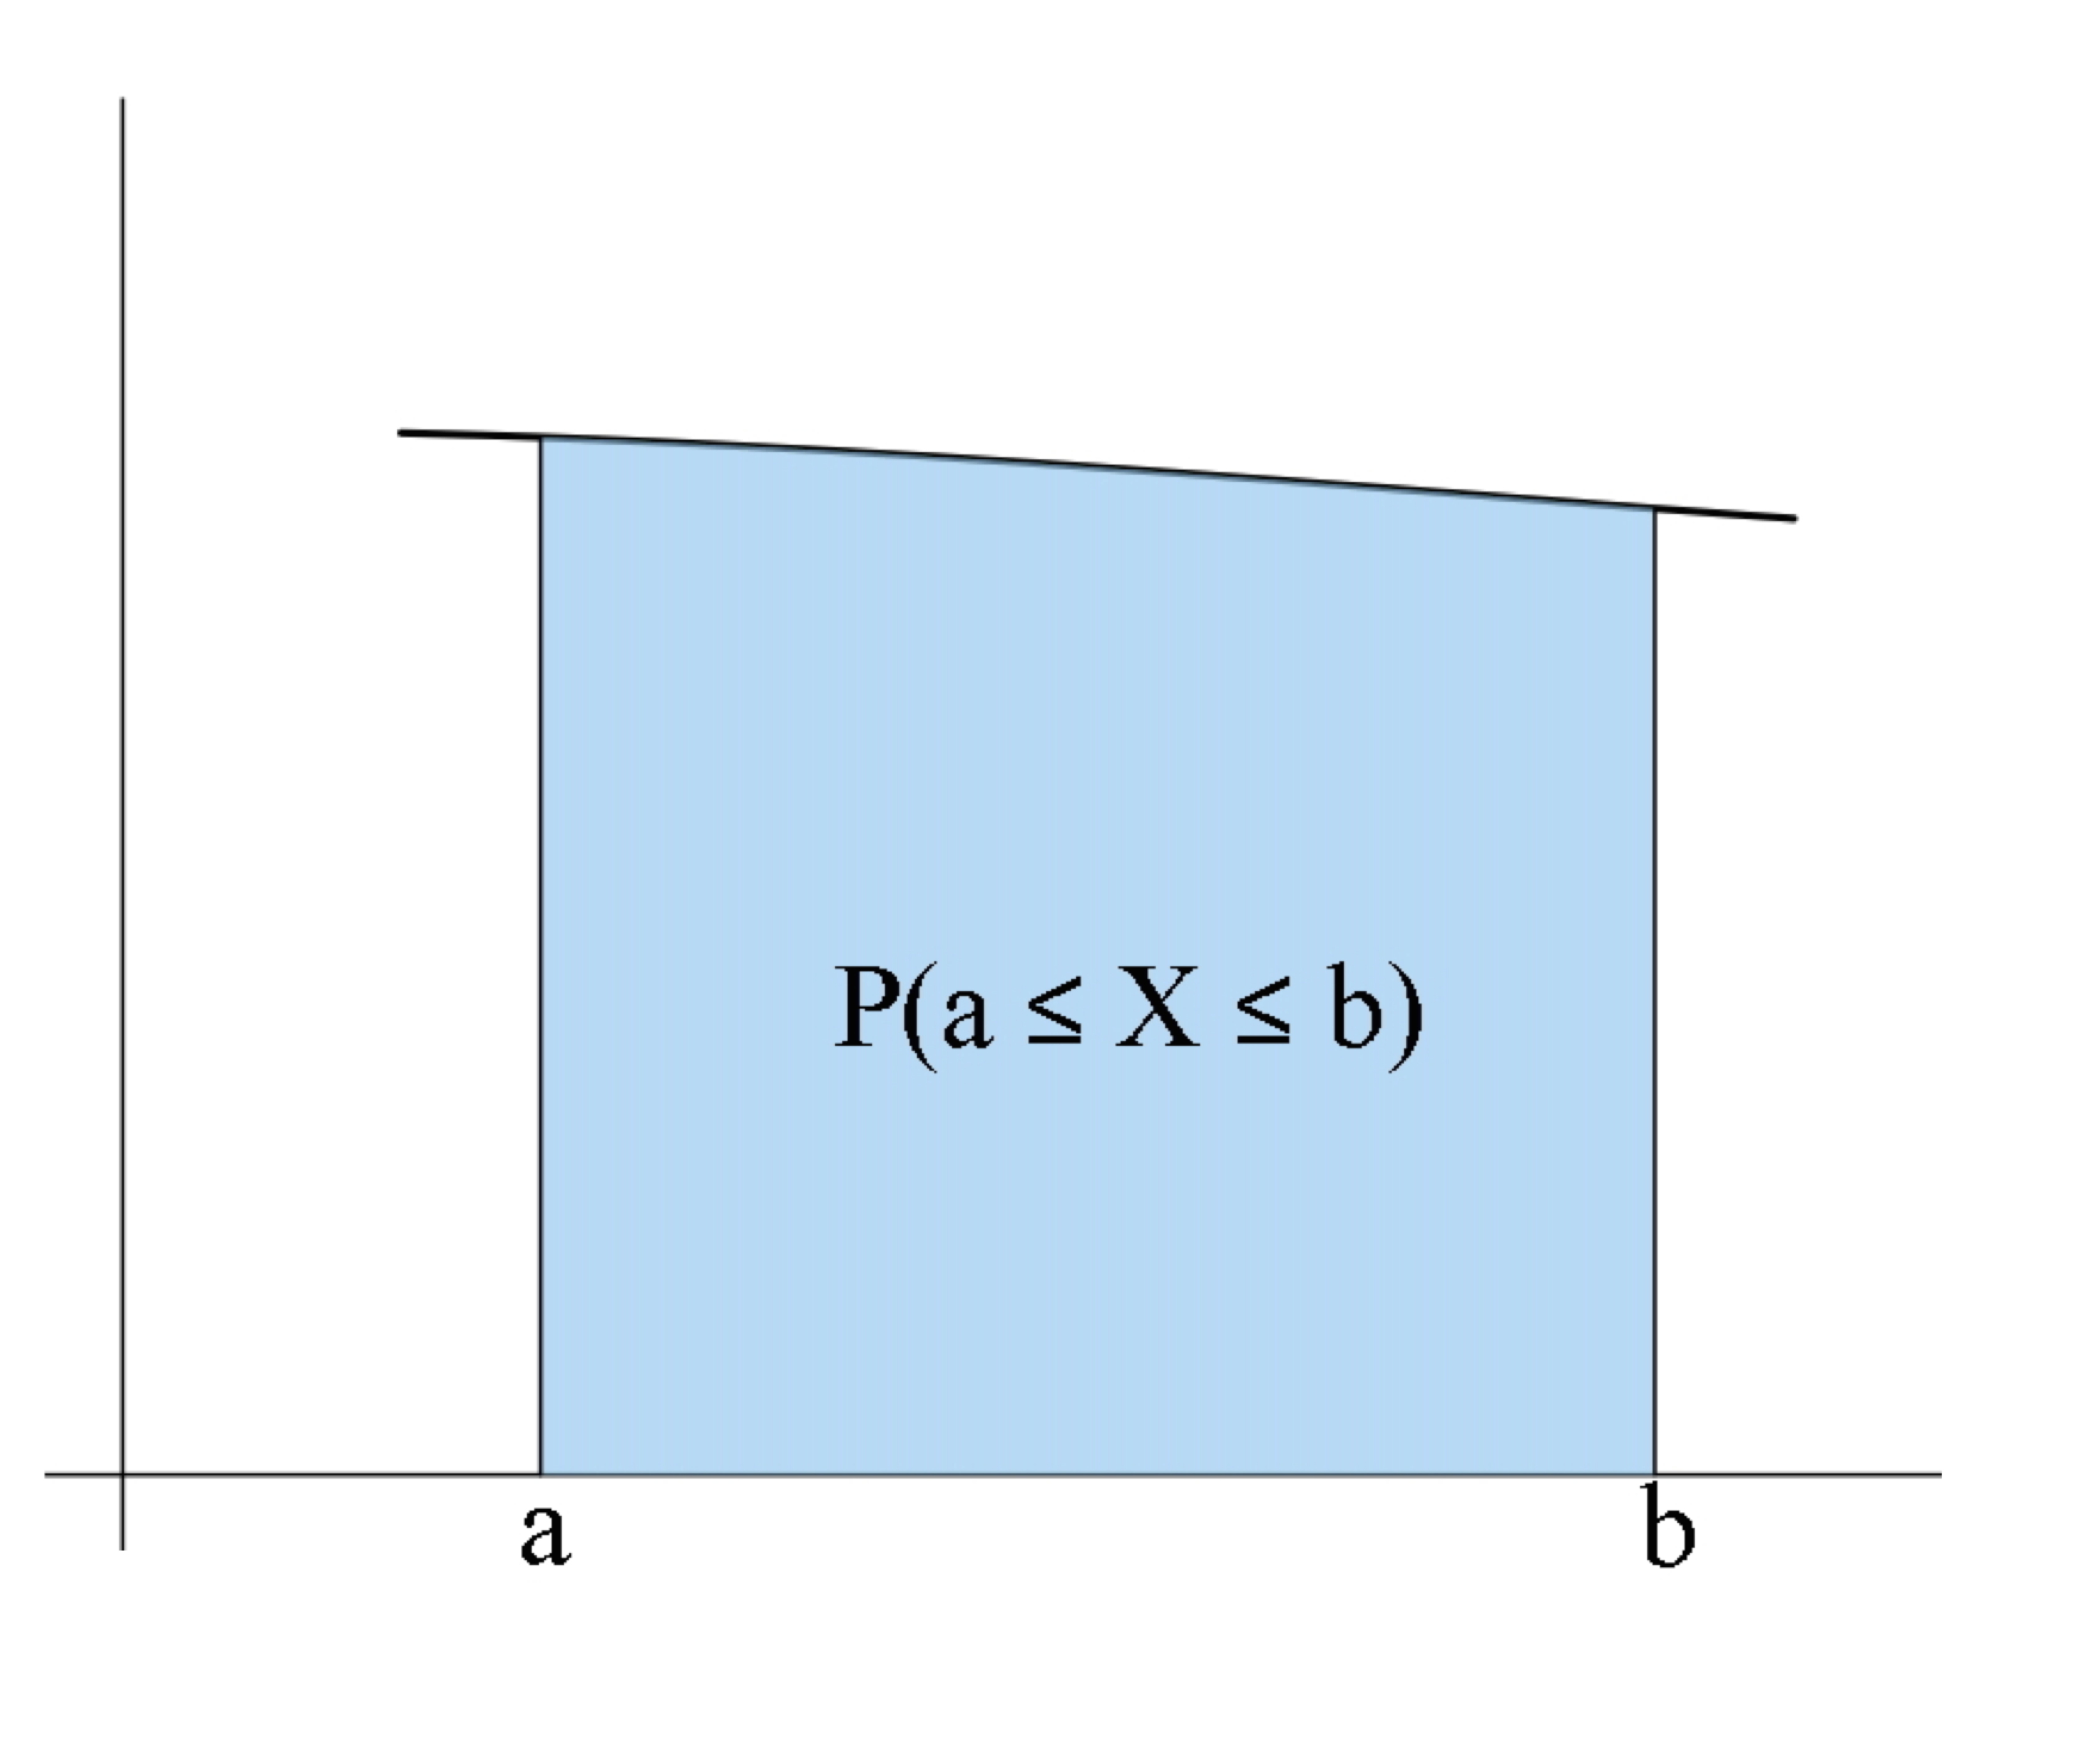
\includegraphics[width=0.6\linewidth]{Bioestadistica-II_files/figure-html/entreaib} \end{center}

\begin{itemize}
\item
  Si \(\varepsilon>0\) és molt, molt petit, l'àrea sota la corba \(y=f_X(x)\) entre \(a-\varepsilon\) i \(a+\varepsilon\) és aproximadament \(2\varepsilon\cdot f_X(a)\) (vegeu la Figura \ref{fig:epsilon}). És a dir,
  \[
  P(a-\varepsilon\leq X\leq a+\varepsilon)\approx 2\varepsilon\cdot f_X(a).
  \]

  Per tant, \(f_X(a)\) ens dóna una indicació de la probabilitat que \(X\) valgui aproximadament \(a\) (però \textbf{no és} \(P(X=a)\), que val 0). És a dir, per exemple, si \(f_X(a)=0.1\) i \(f_X(b)=0.5\), la probabilitat que \(X\) prengui un valor al voltant de \(b\) és 5 vegades més gran que la probabilitat que prengui un valor al voltant d'\(a\).
\end{itemize}

\begin{figure}

{\centering 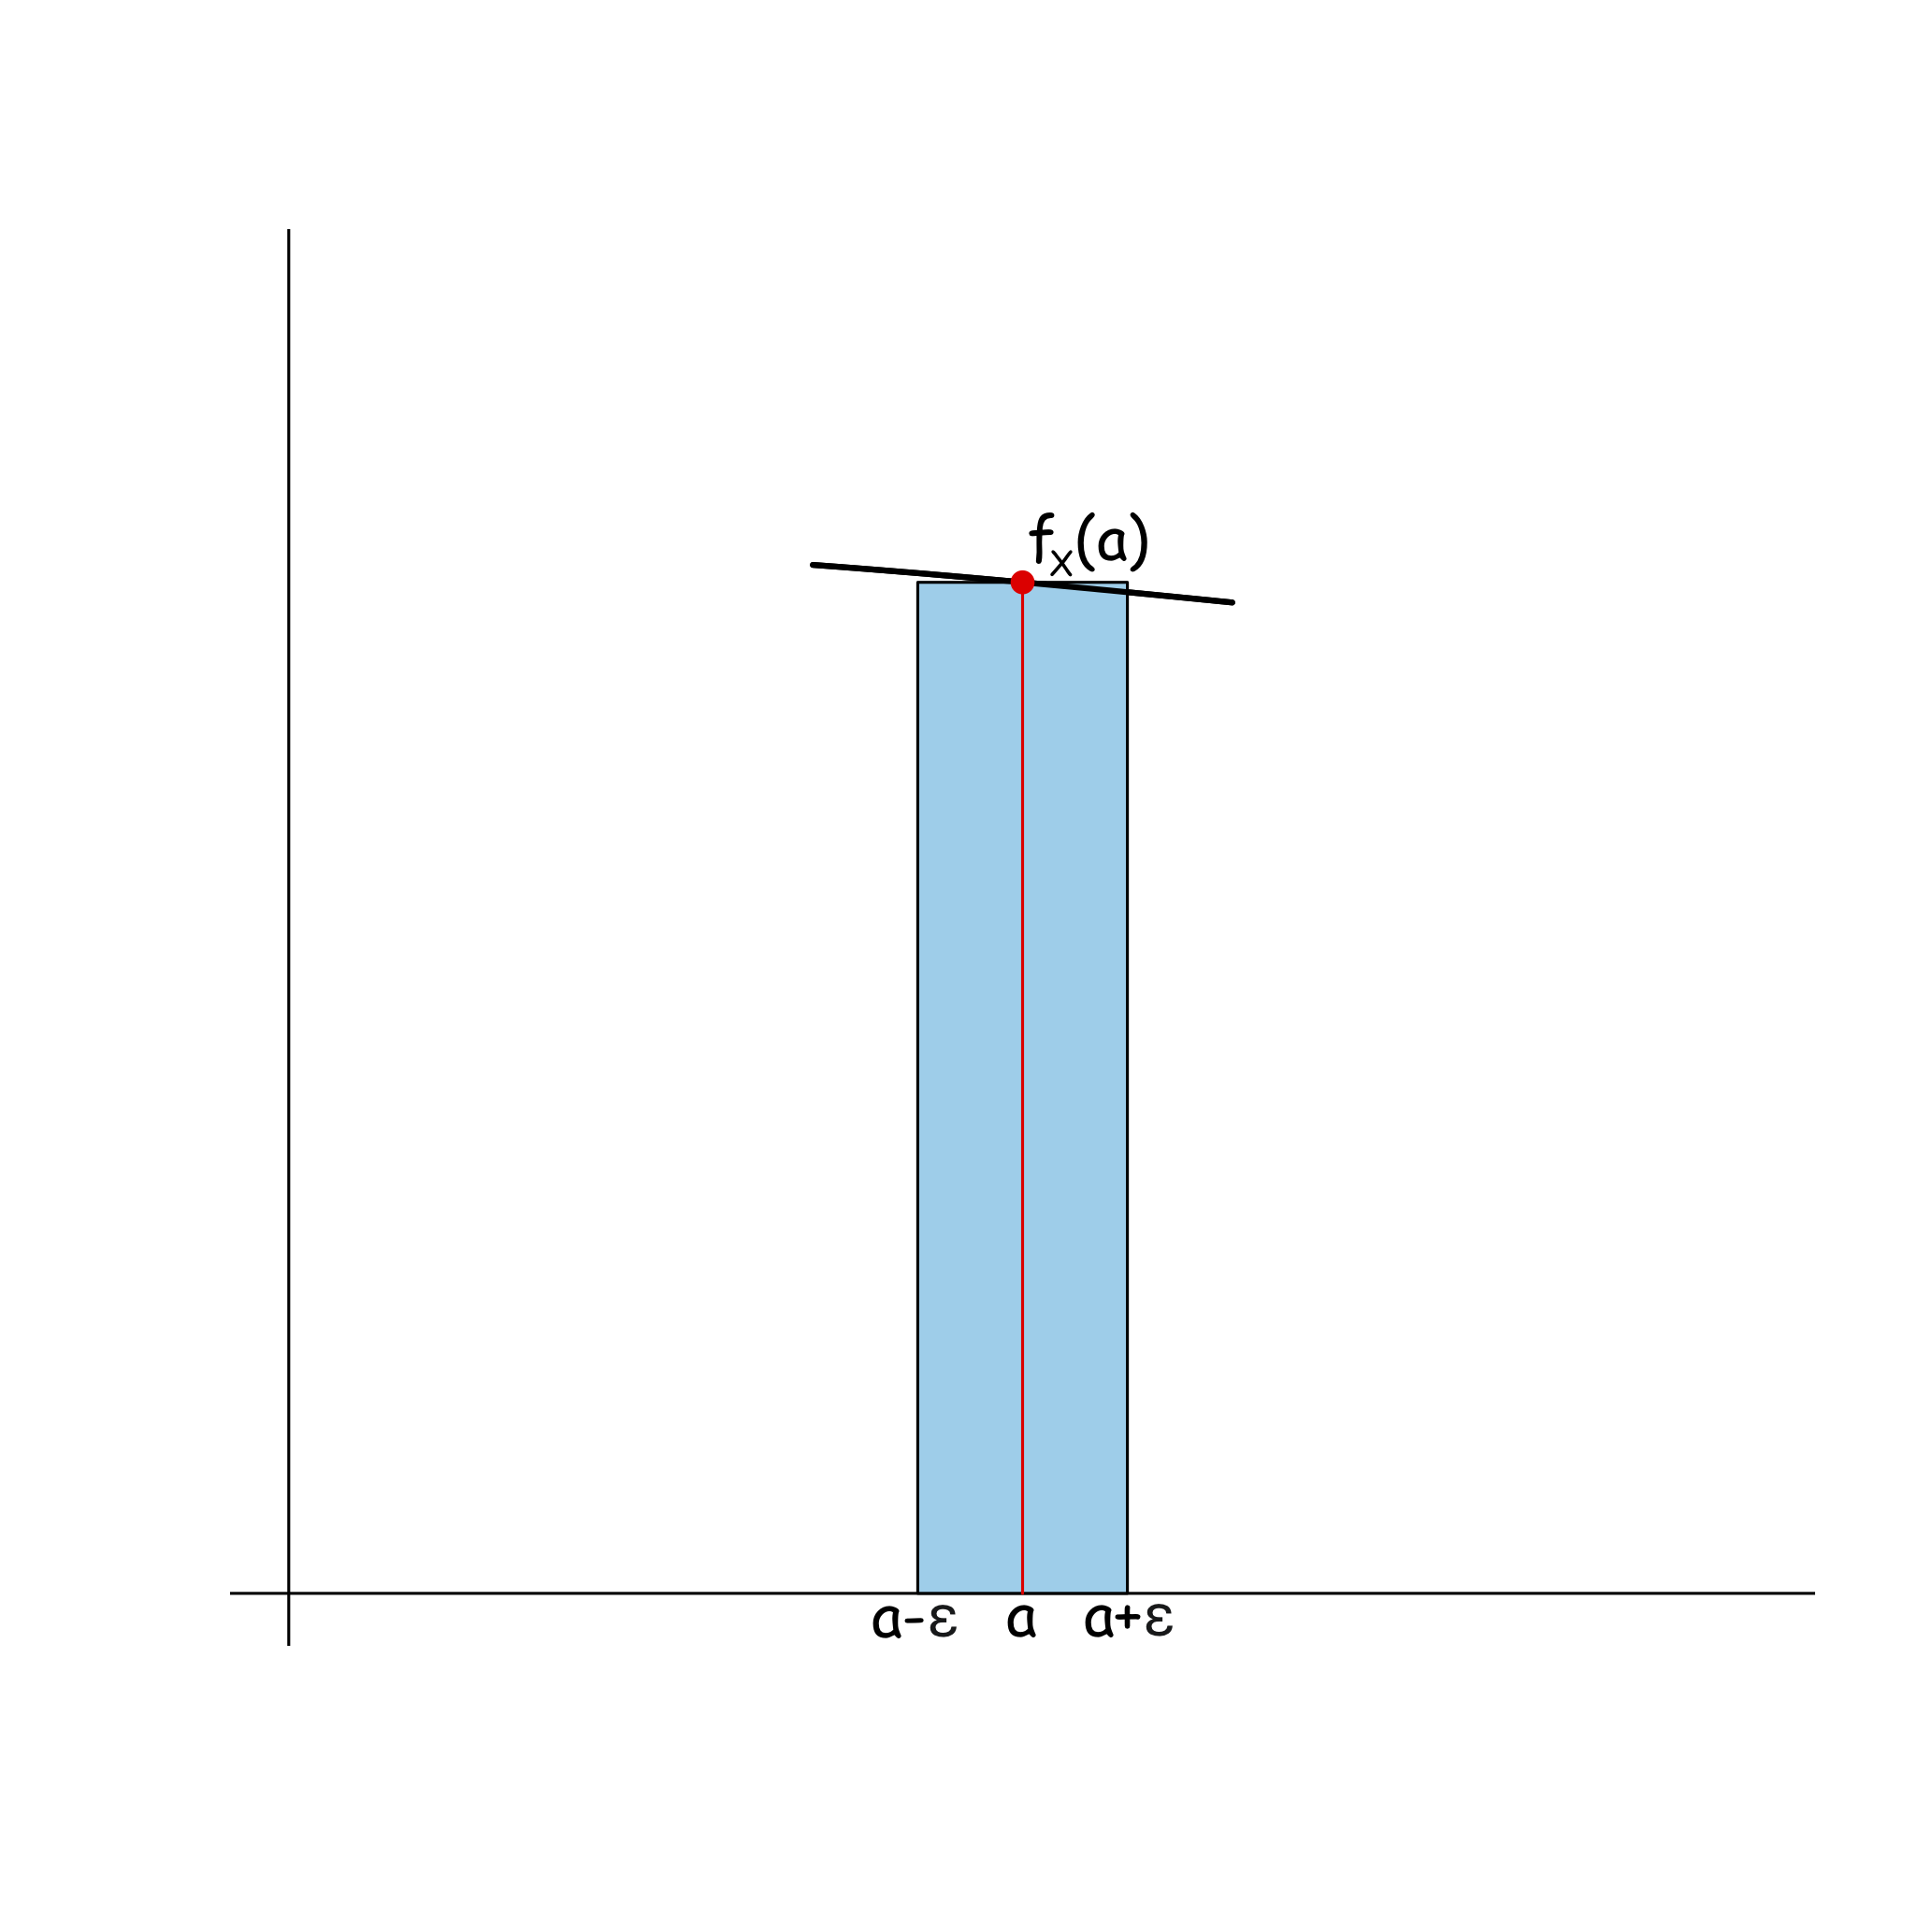
\includegraphics[width=0.6\linewidth]{Bioestadistica-II_files/figure-html/density} 

}

\caption{Àrea sota la corba al voltant d'$a$}\label{fig:epsilon}
\end{figure}

\begin{rmdrecordau}
Però \(P(X=a)=P(X=b)=0\), així que, per favor, evitau dir que ``la probabilitat que \(X\) valgui \(b\) \textbf{és 5 vegades més gran} que la probabilitat que valgui \(a\)''. Sí, ja sabem que \(5\cdot 0=0\), però la frase és enganyosa: la probabilitat que \(X\) valgui \(b\) no més gran que la probabilitat que valgui \(a\).
\end{rmdrecordau}

A les variables aleatòries discretes, definíem la moda com el valor (o els valors) més probable. Però ara no té sentit definir la moda d'una variable contínua \(X\) com el valor \(x_0\) tal que \(P(X=x_0)\) sigui màxim, perquè \(P(X=x)=0\) per a tot \(x\in \mathbb{R}\). Aleshores, es defineix la \textbf{moda} d'una variable aleatòria contínua \(X\) com el valor (o els valors) \(x_0\) tal que \(f_X(x_0)\) és màxim. Com que \(f_X(x_0)\) mesura la probabilitat que \(X\) valgui ``aproximadament'' \(x_0\), tenim que la moda de \(X\) és el valor prop del qual és més probable que caigui el valor de \(X\).

Unes consideracions finals:

\begin{itemize}
\tightlist
\item
  Ho hem dit en la definició, i ho hem emprat implícitament en tota la secció, però ho tornam a repetir: \(f_X(x)\geq 0\) per a tot \(x\in \mathbb{R}\).
\end{itemize}

\begin{rmdcorbes}
En realitat, que \(f_X(x)\) sigui \(\geq 0\) per a tot \(x\in \mathbb{R}\) és conseqüència del fet que la funció \(F_X(x)\) sigui positiva i creixent (les funcions de distribució són sempre creixents, perquè si \(x<y\), \(F_X(x)=P(X\leq x)\leq P(X\leq i)=F_X(y)\)) i coincideixi amb \(\int_{-\infty}^x f_X(x)\,dx\). Però és més senzill donar-ho com a part de la definició i així ens estalviam la demostració.
\end{rmdcorbes}

\begin{itemize}
\tightlist
\item
  \(f_X(x)\) no és una probabilitat, i per tant pot ser més gran que 1. Per exemple, el gràfic següent mostra la densitat d'una variable normal \(N(0,0.01)\) (vegeu la Secció \ref{sec:normal}), que arriba a valer gairebé 40.
\end{itemize}

\begin{center}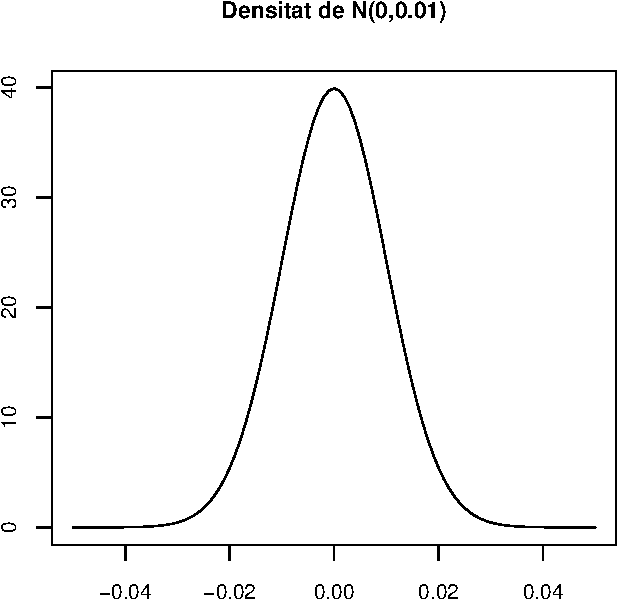
\includegraphics[width=0.6\linewidth]{Bioestadistica-II_files/figure-latex/unnamed-chunk-63-1} \end{center}

\begin{itemize}
\tightlist
\item
  La funció de densitat \(f_X\) no té per què ser contínua, malgrat la funció de distribució \(F_X\) ho sigui.
\end{itemize}

\hypertarget{esperanuxe7a-variuxe0ncia-quantils}{%
\subsection{Esperança, variància, quantils\ldots{}}\label{esperanuxe7a-variuxe0ncia-quantils}}

L'esperança i la variància d'una variable aleatòria contínua \(X\), amb funció de densitat \(f_X\), es defineixen com en el cas discret, substituint la suma \(\sum_{x\in D_x}\) per una integral, i tenen les mateixes propietats.

La \textbf{mitjana}, o \textbf{esperança} (o \textbf{valor mitjà}, \textbf{valor esperat}\ldots), de \(X\) és
\[
E(X)=\int_{-\infty}^{\infty}x \cdot f_{X}(x)\, dx
\]
És a dir, és l'àrea compresa entre l'eix d'abscisses i la corba \(y=xf_X(x)\).
Com en el cas discret, també la indicarem de vegades amb \(\mu_X\).

Aquest valor té la mateixa interpretació que en el cas discret:

\begin{itemize}
\item
  Representa el valor mitjà de \(X\) sobre el total de la població.
\item
  És (amb probabilitat 1) el límit de les mitjanes aritmètica de mostres aleatòries de mida \(n\) de valors de \(X\), quan \(n\to \infty\).
\end{itemize}

Si \(g:\mathbb{R}\to \mathbb{R}\) és una funció contínua, l'\textbf{esperança} de \(g(X)\) és
\[
E(g(X))=\int_{-\infty}^{+\infty} g(x) f_X(x)dx
\]

La \textbf{variància} de \(X\) és
\[
\sigma(X)^2=E((X-\mu_X)^2)=\int_{-\infty}^{+\infty} (x-\mu_X)^2 f_X(x)dx
\]
i es pot demostrar que és igual a
\[
\sigma(X)^2=E(X^2)-\mu_X^2.
\]
També la indicarem de vegades amb \(\sigma_X^2\).

La \textbf{desviació típica} de \(X\) és
\[
\sigma(X)=+\sqrt{\sigma(X)^2}
\]
i també la indicarem de vegades amb \(\sigma_X\).

Com en el cas discret, la variància i la desviació típica quantifiquen la variabilitat dels resultats de \(X\) respecte del seu valor mitjà \(\mu_X\).

Aquests paràmetres de \(X\) tenen les \textbf{mateixes propietats} en el cas continu que en el discret. Les recordam:

\begin{itemize}
\item
  Si \(b\) és una variable aleatòria constant, \(E(b)=b\) i \(\sigma(b)^2=0\).
\item
  Si \(X_1,\ldots,X_n\) són variables aleatòries i \(a_1,\ldots,a_n,b\in \mathbb{R}\),
  \[
  E(a_1X_1+\cdots+a_nX_n+b)=a_1E(X_1)+\cdots+a_nE(X_n)+b
  \]
\item
  Si \(X\leq Y\), aleshores \(E(X)\leq E(Y)\).
\item
  Si \(a,b\in \mathbb{R}\), \(\sigma(aX+b)^2=a^2 \sigma(X)^2\) i \(\sigma(aX+b)=|a|\cdot \sigma(X)\).
\item
  Si \(X_1,\ldots,X_n\) són variables aleatòries \textbf{independents} (i, en principi, només en aquest cas) i \(a_1,\ldots,a_n,b\in \mathbb{R}\),
  \[
  \begin{array}{l}
  \sigma(a_1X_1+\cdots+a_nX_n+b)^2=a_1\cdot\sigma(X_1)^2+\cdots+a_n\cdot\sigma(X_n)^2\\
  \sigma(a_1X_1+\cdots+a_nX_n+b)=\sqrt{a_1\cdot\sigma(X_1)^2+\cdots+a_n\cdot\sigma(X_n)^2}
  \end{array}
  \]
  Si no són independents, aquestes igualtats poden ser falses.
\end{itemize}

El \textbf{quantil d'ordre \(p\)} (o \textbf{\(p\)-quantil}) d'una variable aleatòria contínua \(X\) és el valor \(x_p\in \mathbb{R}\) més petit tal que
\[
F_X(x_p)=P(X\leq x_p)=p
\]

\begin{rmdcorbes}
Observau que, com que \(F_X(x)\) és contínua, tendeix a 0 (la probabilitat del conjunt buit) quan \(x\to -\infty\), i tendeix a 1 (la probabilitat de tot \(\mathbb{R}\)) quan \(x\to +\infty\), pel Teorema del Valor Mitjà de les funcions contínues (que diu, bàsicament, que les funcions contínues no peguen bots) pren tots els valors de l'interval \((0,1)\) i per tant, per a qualsevol \(p\in (0,1)\), existeix qualque \(x\) tal que \(F_X(x)=p\).
\end{rmdcorbes}

La \textbf{mediana} de \(X\) és el seu 0.5-quantil, el \textbf{primer} i \textbf{tercer quartils} són el seu 0.25-quantil i el seu 0.75-quantil, etc.

\hypertarget{sec:normal}{%
\section{Variables aleatòries normals}\label{sec:normal}}

Una variable aleatòria contínua \(X\) és \textbf{normal} (o té distribució normal) \textbf{de paràmetres \(\mu\) i \(\sigma\)} (per abreujar, \(N(\mu,\sigma)\)) quan la seva funció de densitat és
\[
f_{X}(x)=\frac{1}{\sqrt{2\pi}\sigma} e^{{-(x-\mu)^2}/{2\sigma^{2}}}
\]

Naturalment, no us heu de saber aquesta fórmula.

\begin{center}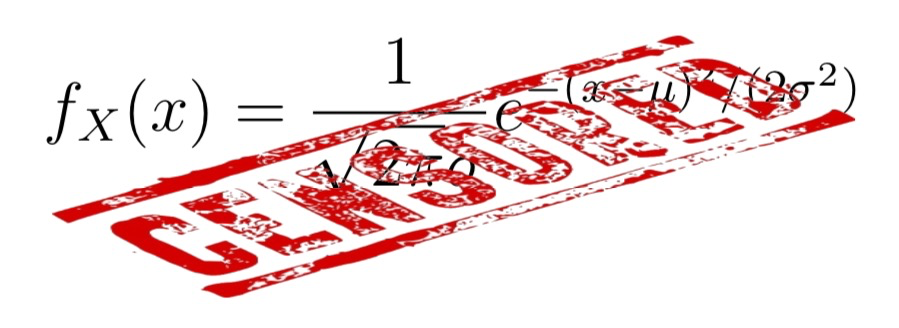
\includegraphics[width=0.35\linewidth]{Bioestadistica-II_files/figure-html/censored} \end{center}

Però sí que heu de saber que:

\begin{itemize}
\item
  Una variable aleatòria normal \(X\) és contínua, i per tant \(P(X=x)=0\), \(P(X\leq x)=P(X<x)\) etc.
\item
  Si \(X\) és normal, la seva funció de distribució \(F_X\) és \textbf{injectiva i creixent}: si \(x<y\), \(F_X(x)<F_X(y)\).
\item
  Si \(X\) és \(N(\mu,\sigma)\), aleshores \(\mu_X=\mu\) i \(\sigma_X=\sigma\).
\end{itemize}

Una variable aleatòria normal diem que és \textbf{estàndard} (o \textbf{típica}) quan és \(N(0,1)\). Normalment indicarem les variables normals estàndard amb \(Z\). Observau, doncs, que si \(Z\) és normal estàndard, \(\mu_Z=0\) i \(\sigma_Z=1\).

La gràfica de la densitat d'una variable aleatòria normal és la famosa \textbf{campana de Gauss}:

\begin{figure}

{\centering 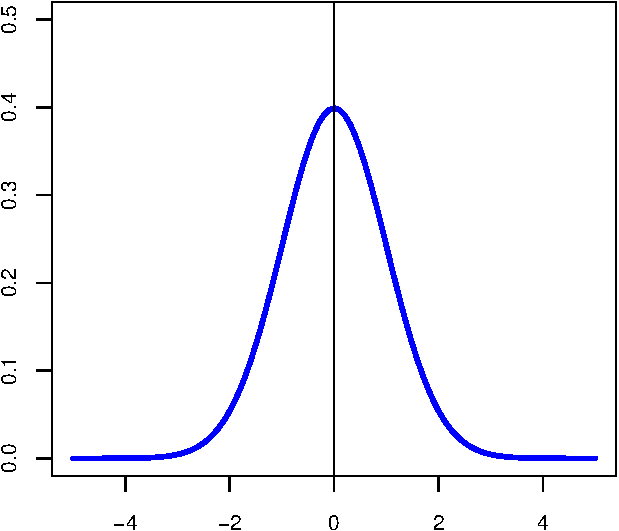
\includegraphics[width=0.5\linewidth]{Bioestadistica-II_files/figure-latex/unnamed-chunk-66-1} 

}

\caption{Densitat d'una variable normal estàndard}\label{fig:unnamed-chunk-66}
\end{figure}

La distribució normal és una distribució teòrica, no la trobareu exacta en la vida real. I malgrat el seu nom, no és més ``normal'' que altres distribucions contínues.

\begin{center}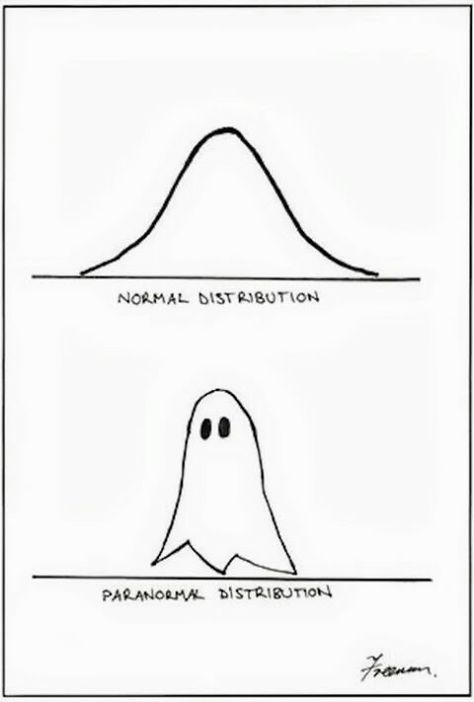
\includegraphics[width=0.4\linewidth]{Bioestadistica-II_files/figure-html/paranormal} \end{center}

Però és molt important, pel fet que moltes distribucions de la vida real són aproximadament normals. El motiu és que:

\begin{quote}
Si una variable aleatòria consisteix a prendre un nombre \textbf{molt gran} \(n\) de mesures independents d'una o diverses variables aleatòries i sumar-les, aleshores té distribució aproximadament normal, encara que les variables aleatòries de partida no ho siguin.
\end{quote}

\begin{example}
\protect\hypertarget{exm:unnamed-chunk-68}{}{\label{exm:unnamed-chunk-68} }Una variable binomial \(B(n,p)\) s'obté prenent \(n\) mesures independents d'una variable Bernoulli \(Be(p)\) i sumant-les. Per tant, per la ``regla'' anterior, una \(B(n,p)\) hauria de ser aproximadament normal si \(n\) és gran. Doncs sí, si \(n\) és gran (posem més gran que 40, encara que si \(p\) és molt propera a 0 o 1, la mida de les mostres ha de ser més gran), una variable \(X\) binomial \(B(n,p)\) és aproximadament normal \(N(np,\sqrt{np(1-p)})\), on, recordau que si \(X\) és \(B(n,p)\), aleshores \(\mu_X=np\) i \(\sigma_X=\sqrt{np(1-p)}\). Aquest ``aproximadament'' significa que la densitat i la distribució de \(X\) són aproximadament les de la normal.
\end{example}

Per exemple, el gràfic següent compara les funcions de distribució d'una binomial \(B(40,0.3)\) i una normal \(N(40\cdot 0.3,\sqrt{40\cdot 0.3\cdot 0.7})\).

\begin{figure}

{\centering 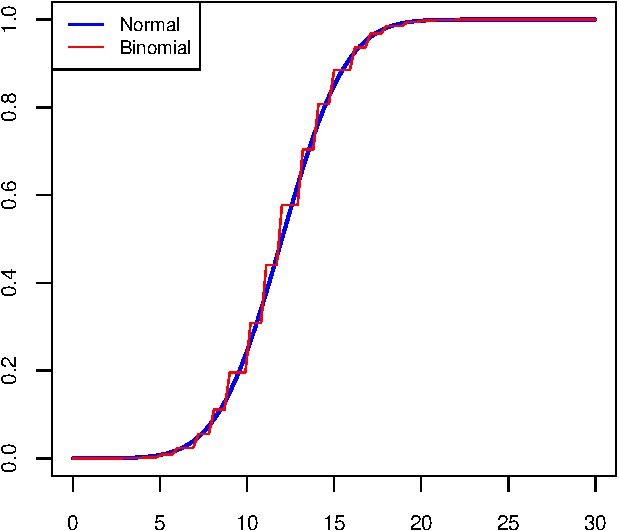
\includegraphics[width=0.5\linewidth]{Bioestadistica-II_files/figure-latex/unnamed-chunk-69-1} 

}

\caption{Funcions de distribució de B(40,0.3) i N(400.3,sqrt(500.30.7)}\label{fig:unnamed-chunk-69}
\end{figure}

\begin{rmdrecordau}
En els propers temes emprarem sovint que una variable \(B(n,p)\) amb \(n\) és gran és aproximadament \(N(np,\sqrt{np(1-p)})\).
\end{rmdrecordau}

\begin{example}
\protect\hypertarget{exm:unnamed-chunk-71}{}{\label{exm:unnamed-chunk-71} }Podem entendre que, amb una variable de Poisson, observam tots els punts d'un espai o tots els instants d'un període de temps i sumam tots els Èxits que hi trobam. Doncs, un altre cop, si \(X\) és una variable aleatòria de Poisson \(Po(\lambda)\) i \(\lambda\) és gran, aleshores \(X\) és aproximadament \(N(\lambda,\sqrt{\lambda})\).
\end{example}

Per exemple, el gràfic següent compara les funcions de distribució d'una Poisson \(Po(70)\) i una normal \(N(70,\sqrt{70})\).

\begin{figure}

{\centering 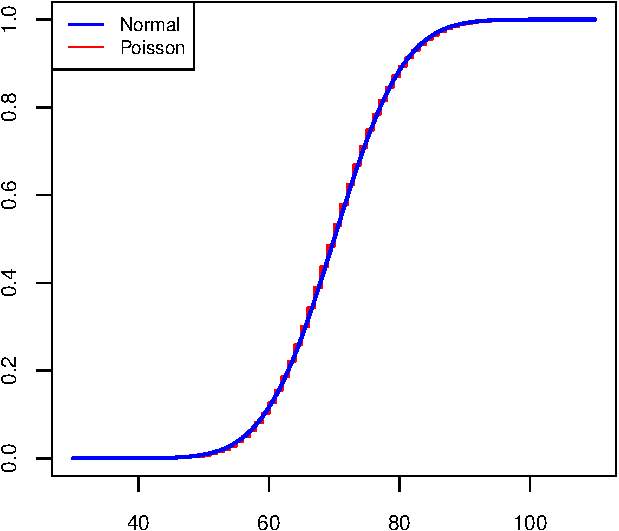
\includegraphics[width=0.5\linewidth]{Bioestadistica-II_files/figure-latex/unnamed-chunk-72-1} 

}

\caption{Funcions de distribució de Pois(70) i N(70,sqrt(70))}\label{fig:unnamed-chunk-72}
\end{figure}

\begin{rmdcaution}
Quan s'aproxima una variable discreta \(X\), com ara una binomial o una Poisson, per mitjà d'una variable normal \(Y\), és convenient aplicar l'anomenada \textbf{correcció de continuïtat}: per a cada \(n\in \mathbb{N}\), aproximar:

\begin{itemize}
\item
  \(P(X\leq n)\) per mitjà de \(P(Y< n+1/2)\)
\item
  \(P(X=n)\) per mitjà de \(P(n-1/2< Y< n+1/2)\)
\end{itemize}

Vegeu l'Exemple \ref{exm:corrcont} més a baix.
\end{rmdcaution}

\hypertarget{amb-r}{%
\subsection{Amb R}\label{amb-r}}

Per calcular probabilitats d'una \(N(\mu,\sigma)\), cal calcular les integrals a mà.

\begin{center}
\includegraphics[width=0.2\linewidth]{Bioestadistica-II_files/figure-html/emorisa} \end{center}

O podeu usar R, per a qui la normal és \texttt{norm}. Per tant, si \(X\sim N(\mu,\sigma)\):

\begin{itemize}
\item
  \texttt{dnorm(x,mu,sigma)} dóna el valor de la densitat \(f_X(x)\)
\item
  \texttt{pnorm(x,mu,sigma)} dóna el valor de la distribució \(F_X(x)=P(X\leq x)\)
\item
  \texttt{qnorm(q,mu,sigma)} dóna el \(q\)-quantil de \(X\)
\item
  \texttt{rnorm(n,mu,sigma)} dóna un vector de \(n\) nombres aleatoris generats amb aquesta distribució
\end{itemize}

Així, per exemple, si \(X\) és \(N(1,2)\)

\begin{itemize}
\tightlist
\item
  \(P(X\leq 1.5)\) és
\end{itemize}

\begin{Shaded}
\begin{Highlighting}[]
\FunctionTok{pnorm}\NormalTok{(}\FloatTok{1.5}\NormalTok{,}\DecValTok{1}\NormalTok{,}\DecValTok{2}\NormalTok{)}
\end{Highlighting}
\end{Shaded}

\begin{verbatim}
## [1] 0.5987063
\end{verbatim}

\begin{itemize}
\tightlist
\item
  El 0.4-quantil de \(X\), és a dir, el valor \(q\) tal que \(P(X\leq q)=0.4\) és
\end{itemize}

\begin{Shaded}
\begin{Highlighting}[]
\FunctionTok{qnorm}\NormalTok{(}\FloatTok{0.4}\NormalTok{,}\DecValTok{1}\NormalTok{,}\DecValTok{2}\NormalTok{)}
\end{Highlighting}
\end{Shaded}

\begin{verbatim}
## [1] 0.4933058
\end{verbatim}

\begin{itemize}
\tightlist
\item
  \(P(X=1.5)\) és
\end{itemize}

\begin{Shaded}
\begin{Highlighting}[]
\FunctionTok{dnorm}\NormalTok{(}\FloatTok{1.5}\NormalTok{,}\DecValTok{1}\NormalTok{,}\DecValTok{2}\NormalTok{)}
\end{Highlighting}
\end{Shaded}

\begin{verbatim}
## [1] 0.1933341
\end{verbatim}

\begin{rmderror}
No! Com que \(X\) és contínua, \(P(X=1.5)=0\). El que us dóna \texttt{dnorm(1.5,1,2)} és el valor de la funció de densitat de \(X\) en 1.5, que no creiem que us interessi gaire.
\end{rmderror}

Si la normal és estàndard, no fa falta entrar la \(\mu=0\) i la \(\sigma=1\) (són els valors per defecte d'aquests paràmetres per a \texttt{norm}). Així, si \(Z\) és \(N(0,1)\):

\begin{itemize}
\tightlist
\item
  \(P(Z\leq 1.5)\) és
\end{itemize}

\begin{Shaded}
\begin{Highlighting}[]
\FunctionTok{pnorm}\NormalTok{(}\FloatTok{1.5}\NormalTok{)}
\end{Highlighting}
\end{Shaded}

\begin{verbatim}
## [1] 0.9331928
\end{verbatim}

\begin{itemize}
\tightlist
\item
  El seu 0.95-quantil és
\end{itemize}

\begin{Shaded}
\begin{Highlighting}[]
\FunctionTok{qnorm}\NormalTok{(}\FloatTok{0.95}\NormalTok{)}
\end{Highlighting}
\end{Shaded}

\begin{verbatim}
## [1] 1.644854
\end{verbatim}

\begin{itemize}
\tightlist
\item
  Què val \(P(-1\leq Z\leq 1)\)? Com que \(P(-1\leq Z\leq 1)=P(Z\leq 1)-P(Z\leq -1)\), és
\end{itemize}

\begin{Shaded}
\begin{Highlighting}[]
\FunctionTok{pnorm}\NormalTok{(}\DecValTok{1}\NormalTok{)}\SpecialCharTok{{-}}\FunctionTok{pnorm}\NormalTok{(}\SpecialCharTok{{-}}\DecValTok{1}\NormalTok{)}
\end{Highlighting}
\end{Shaded}

\begin{verbatim}
## [1] 0.6826895
\end{verbatim}

\begin{example}
\protect\hypertarget{exm:corrcont}{}{\label{exm:corrcont} }A la secció anterior, us hem dit que una variable binomial \(B(n,p)\) amb \(n\) gran s'aproxima per mitjà d'una variable normal \(N(np,\sqrt{np(1-p)})\). Així, per exemple, una variable \(X\) binomial \(B(400,0.2)\) s'aproxima per mitjà d'una variable \(Y\) normal \(N(400\cdot 0.2,\sqrt{400\cdot 0.2\cdot 0.8})=N(80,8)\). Vegem amb alguns exemples que aquesta aproximació és millor aplicant-hi la correcció de continuïtat:
\end{example}

\begin{itemize}
\tightlist
\item
  \(F_X(70)=P(X\leq 70)\):
\end{itemize}

\begin{Shaded}
\begin{Highlighting}[]
\FunctionTok{pbinom}\NormalTok{(}\DecValTok{70}\NormalTok{,}\DecValTok{400}\NormalTok{,}\FloatTok{0.2}\NormalTok{)}
\end{Highlighting}
\end{Shaded}

\begin{verbatim}
## [1] 0.1163917
\end{verbatim}

\begin{itemize}
\tightlist
\item
  \(F_Y(70)=P(Y\leq 70)\):
\end{itemize}

\begin{Shaded}
\begin{Highlighting}[]
\FunctionTok{pnorm}\NormalTok{(}\DecValTok{70}\NormalTok{,}\DecValTok{80}\NormalTok{,}\DecValTok{8}\NormalTok{)}
\end{Highlighting}
\end{Shaded}

\begin{verbatim}
## [1] 0.1056498
\end{verbatim}

\begin{itemize}
\tightlist
\item
  L'aproximació de continuïtat ens diu que és millor aproximar \(P(X\leq 70)\) per mitjà de \(P(Y< 70+1/2)\):
\end{itemize}

\begin{Shaded}
\begin{Highlighting}[]
\FunctionTok{pnorm}\NormalTok{(}\FloatTok{70.5}\NormalTok{,}\DecValTok{80}\NormalTok{,}\DecValTok{8}\NormalTok{)}
\end{Highlighting}
\end{Shaded}

\begin{verbatim}
## [1] 0.1175152
\end{verbatim}

\begin{itemize}
\tightlist
\item
  \(f_X(70)=P(X=70)\):
\end{itemize}

\begin{Shaded}
\begin{Highlighting}[]
\FunctionTok{dbinom}\NormalTok{(}\DecValTok{70}\NormalTok{,}\DecValTok{400}\NormalTok{,}\FloatTok{0.2}\NormalTok{) }
\end{Highlighting}
\end{Shaded}

\begin{verbatim}
## [1] 0.02338443
\end{verbatim}

\begin{itemize}
\tightlist
\item
  \(f_Y(70)\) (que \textbf{no és} \(P(Y=70)\):
\end{itemize}

\begin{Shaded}
\begin{Highlighting}[]
\FunctionTok{dnorm}\NormalTok{(}\DecValTok{70}\NormalTok{,}\DecValTok{80}\NormalTok{,}\DecValTok{8}\NormalTok{) }
\end{Highlighting}
\end{Shaded}

\begin{verbatim}
## [1] 0.02283114
\end{verbatim}

\begin{itemize}
\tightlist
\item
  L'aproximació de continuïtat ens diu que és millor aproximar \(P(X=70)\) per mitjà de \(P(70-1/2<Y< 70+1/2)\):
\end{itemize}

\begin{Shaded}
\begin{Highlighting}[]
\FunctionTok{pnorm}\NormalTok{(}\FloatTok{70.5}\NormalTok{,}\DecValTok{80}\NormalTok{,}\DecValTok{8}\NormalTok{) }\SpecialCharTok{{-}}\FunctionTok{pnorm}\NormalTok{(}\FloatTok{69.5}\NormalTok{,}\DecValTok{80}\NormalTok{,}\DecValTok{8}\NormalTok{)}
\end{Highlighting}
\end{Shaded}

\begin{verbatim}
## [1] 0.02283949
\end{verbatim}

\begin{example}
\protect\hypertarget{exm:exhiperhipo}{}{\label{exm:exhiperhipo} }La pressió sistòlica, mesurada en mm Hg, es distribueix com una variable normal amb valor mitjà i desviació típica que depenen del sexe i l'edat. Per a la franja d'edat 16-24 anys, aquests valors (s'estima que) són:

\begin{itemize}
\tightlist
\item
  Per a homes, \(\mu=124\) i \(\sigma=13.7\)
\item
  Per a dones, \(\mu=117\) i \(\sigma=13.7\)
\end{itemize}

El model d'hipertensió-hipotensió acceptat és el descrit en la Figura \ref{fig:hiperhipo}. Volem calcular els límits de cada classe per a cada sexe en aquest grup d'edat.
\end{example}

\begin{figure}

{\centering 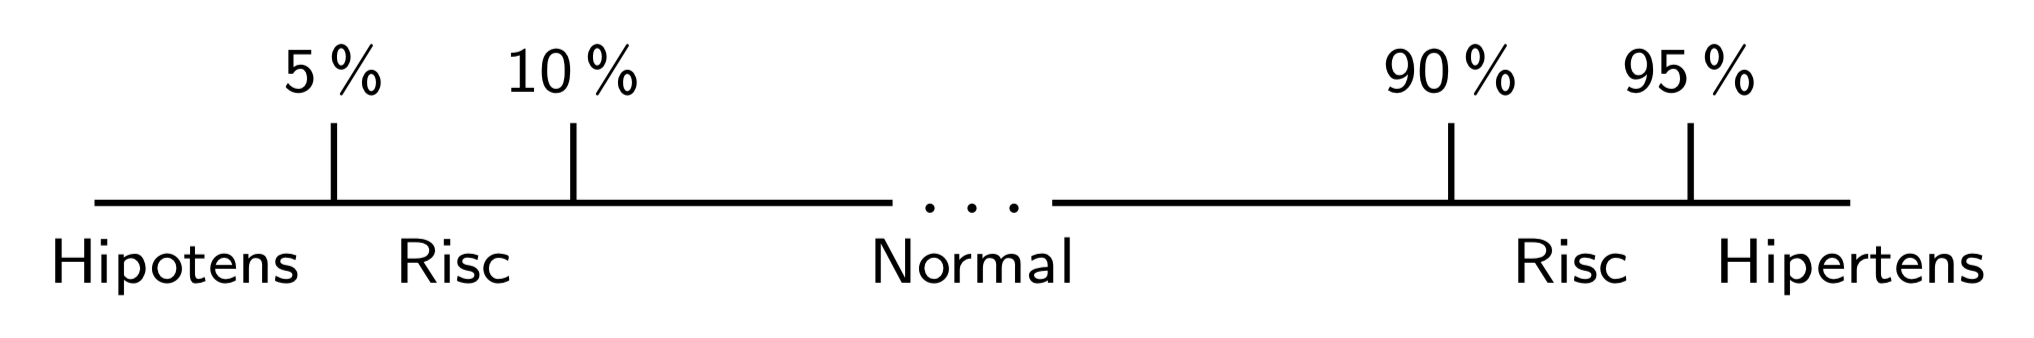
\includegraphics[width=0.8\linewidth]{Bioestadistica-II_files/figure-html/hiperhipo} 

}

\caption{Model d'hipertensió-hipotensió.}\label{fig:hiperhipo}
\end{figure}

Vegem:

\begin{itemize}
\tightlist
\item
  El límit superior del grup d'hipotensió serà el valor que deixa a l'esquerra un 5\% de les tensions: el 0.05-quantil de la distribució.
\item
  El límit superior del grup de risc d'hipotensió serà el valor que deixa a l'esquerra un 10\% de les tensions: el 0.1-quantil de la distribució.
\item
  El límit inferior del grup de risc d'hipertensió serà el valor que deixa a l'esquerra un 90\% de les tensions: el 0.9-quantil de la distribució.
\item
  El límit inferior del grup d'hipertensió serà el valor que deixa a l'esquerra un 95\% de les tensions: el 0.95-quantil de la distribució.
\end{itemize}

En els homes, la tensió sistòlica és una variable aleatòria \(N(124,13.7)\). Aleshores, aquests quantils són:

\begin{itemize}
\tightlist
\item
  El 0.05-quantil:
\end{itemize}

\begin{Shaded}
\begin{Highlighting}[]
\FunctionTok{qnorm}\NormalTok{(}\FloatTok{0.05}\NormalTok{,}\DecValTok{124}\NormalTok{,}\FloatTok{13.7}\NormalTok{)}
\end{Highlighting}
\end{Shaded}

\begin{verbatim}
## [1] 101.4655
\end{verbatim}

\begin{itemize}
\tightlist
\item
  El 0.1-quantil:
\end{itemize}

\begin{Shaded}
\begin{Highlighting}[]
\FunctionTok{qnorm}\NormalTok{(}\FloatTok{0.1}\NormalTok{,}\DecValTok{124}\NormalTok{,}\FloatTok{13.7}\NormalTok{)}
\end{Highlighting}
\end{Shaded}

\begin{verbatim}
## [1] 106.4427
\end{verbatim}

\begin{itemize}
\tightlist
\item
  El 0.9-quantil:
\end{itemize}

\begin{Shaded}
\begin{Highlighting}[]
\FunctionTok{qnorm}\NormalTok{(}\FloatTok{0.9}\NormalTok{,}\DecValTok{124}\NormalTok{,}\FloatTok{13.7}\NormalTok{)}
\end{Highlighting}
\end{Shaded}

\begin{verbatim}
## [1] 141.5573
\end{verbatim}

\begin{itemize}
\tightlist
\item
  El 0.95-quantil:
\end{itemize}

\begin{Shaded}
\begin{Highlighting}[]
\FunctionTok{qnorm}\NormalTok{(}\FloatTok{0.95}\NormalTok{,}\DecValTok{124}\NormalTok{,}\FloatTok{13.7}\NormalTok{)}
\end{Highlighting}
\end{Shaded}

\begin{verbatim}
## [1] 146.5345
\end{verbatim}

En resum, per als homes de 16 a 24 anys tenim els límits de la Taula \ref{tab:tensio}.

\begin{table}

\caption{\label{tab:tensio}Límits d'hipotensió-hipertensió en homes joves.}
\centering
\begin{tabular}[t]{l|l}
\hline
Grup & Interval\\
\hline
Hipotens & <101.5\\
\hline
Prehipotens & 101.5 a 106.4\\
\hline
Normotens & 106.4 a 141.6\\
\hline
Prehipertens & 141.6 a 146.5\\
\hline
Hipertens & > 146.5\\
\hline
\end{tabular}
\end{table}

\begin{rmdexercici}
Calculau els límits per a les dones.
\end{rmdexercici}

\hypertarget{propietats-buxe0siques}{%
\subsection{Propietats bàsiques}\label{propietats-buxe0siques}}

Una de les propietats clau de la distribució normal és la seva simetria:

\begin{rmdimportant}
Si \(X\) és \(N(\mu,\sigma)\), la seva densitat \(f_X\) és simètrica respecte de \(\mu\), és a dir,
\[
f_{X}(\mu-x)=f_{X}(\mu+x),
\]
i pren el valor màxim a \(x=\mu\). És a dir, \(\mu\) és la \textbf{moda} de \(X\).
\end{rmdimportant}

\begin{center}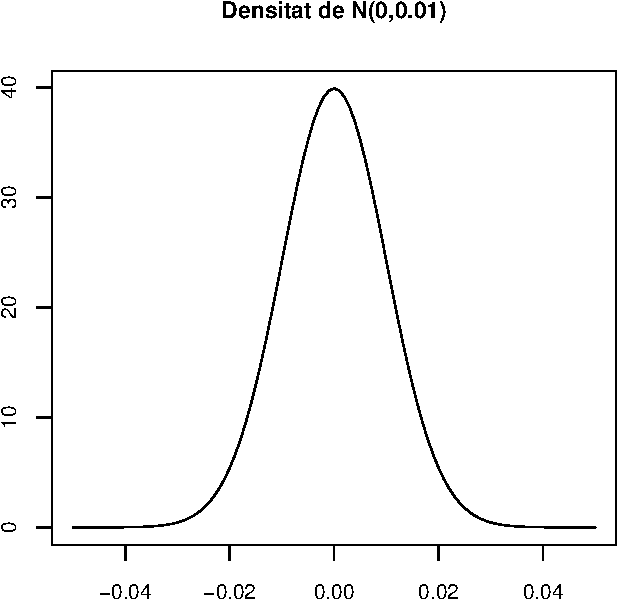
\includegraphics[width=0.8\linewidth]{Bioestadistica-II_files/figure-latex/unnamed-chunk-95-1} \end{center}

Per tant, el valor al voltant del qual és més probable que una variable normal \(N(\mu,\sigma)\) caigui és el seu valor esperat \(\mu\).

En particular, si \(Z\) és \(N(0,1)\), llavors \(f_Z\) és simètrica al voltant de 0, és a dir, \(f_{Z}(-x)=f_{Z}(x)\), i la moda de \(Z\) és \(x=0\).

Recordau que la funció de distribució d'una variable aleatòria contínua \(X\),
\[
F_X(x)=P(X\leq x)
\]
és l'àrea compresa entre la densitat \(y=f_X(x)\) i l'eix d'abscisses a l'esquerra de \(x\).

\begin{center}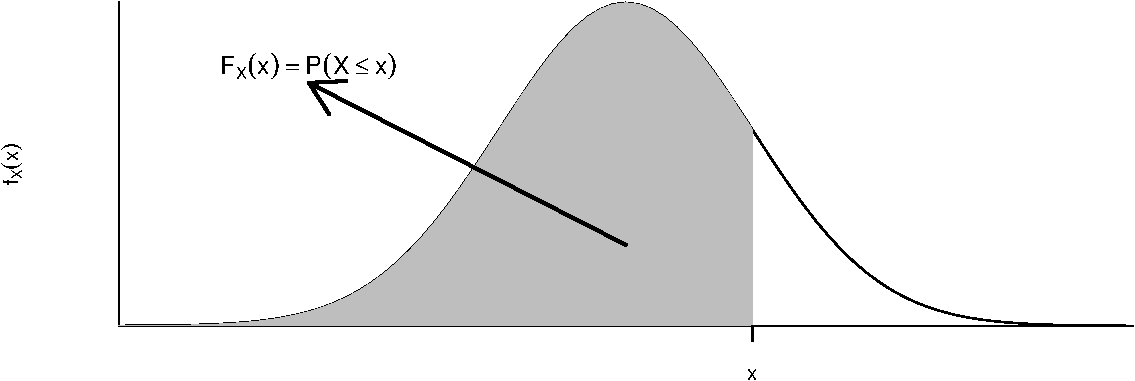
\includegraphics[width=0.8\linewidth]{Bioestadistica-II_files/figure-latex/unnamed-chunk-96-1} \end{center}

Llavors, la simetria de \(f_X\) fa que, per a tot \(x\geq 0\), les àrees a l'esquerra de \(\mu-x\) i a la dreta de \(\mu+x\) siguin iguals.

\begin{center}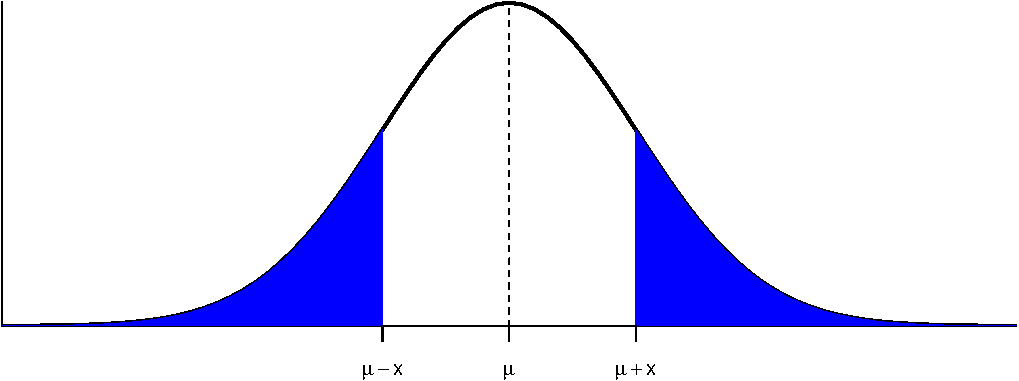
\includegraphics[width=0.8\linewidth]{Bioestadistica-II_files/figure-latex/unnamed-chunk-97-1} \end{center}

És a dir,
\[
P(X\leq \mu-x)=P(X\geq \mu+x)=1-P(X\leq \mu+x)
\]

En particular (prenent \(x=0\))
\[
P(X\leq \mu)=1-P(X\leq \mu)\Rightarrow P(X\leq \mu)=0.5
\]
i per tant, \(\mu\) és també la \textbf{mediana} de \(X\).

\begin{rmdimportant}
Si \(X\) és \(N(\mu,\sigma)\), \(\mu\) és la mitjana, la mediana i la moda de \(X\).
\end{rmdimportant}

En el cas concret de la normal estàndard \(Z\), per a qualsevol \(z\geq 0\) es té que les àrees a l'esquerra de \(-z\) i a la dreta de \(z\) són iguals
\[
P(Z\leq -z)=P(Z\geq z)=1-P(Z\leq z)
\]
i la mediana de \(Z\) és 0.

\begin{rmdnote}
Ara que sabem més coses de la normal, a l'Exemple \ref{exm:exhiperhipo} ens haguéssim pogut estalviar la meitat de la feina: per la simetria, el 0.95-quantil ha d'estar a la mateixa distància de \(\mu\) que el 0.05-quantil, però a la dreta. És a dir, com que \(\mu=124\) i el 0.05-quantil havia estat 101.4655, el 0.95-quantil ha de ser el valor a la dreta de 124 i a la mateixa distància d'aquest que 101.4655:
\[
124+(124-101.4655)=126.5345
\]
El mateix passa amb el 0.9-quantil i el 0.1-quantil, comprovau-ho.
\end{rmdnote}

Si \(\mu\) creix, desplaça a la dreta l'eix vertical de simetria de la densitat, i amb ell tota la corba.

\begin{center}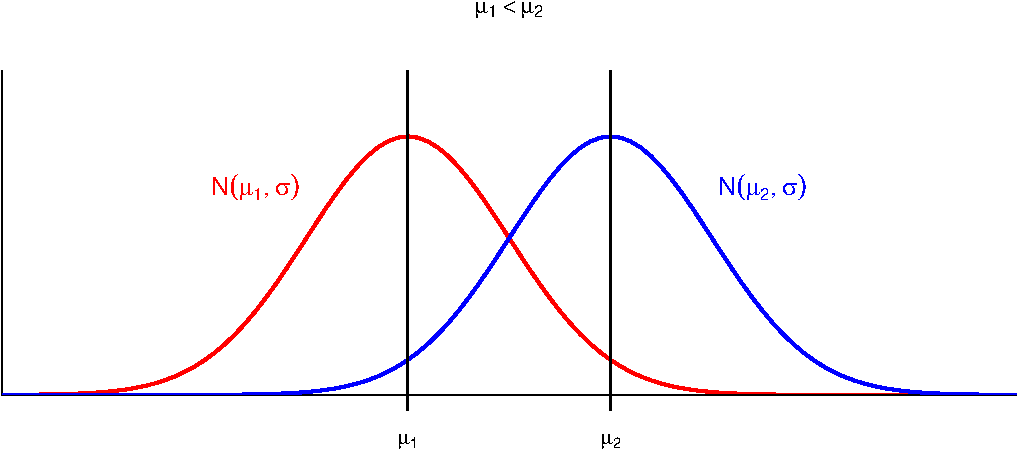
\includegraphics[width=0.8\linewidth]{Bioestadistica-II_files/figure-latex/unnamed-chunk-101-1} \end{center}

Si \(\sigma\) creix, la corba s'aplana: en augmentar la desviació típica, els valors són més variats i augmenta la probabilitat que prenguin valors més llunays de \(\mu\).

\begin{center}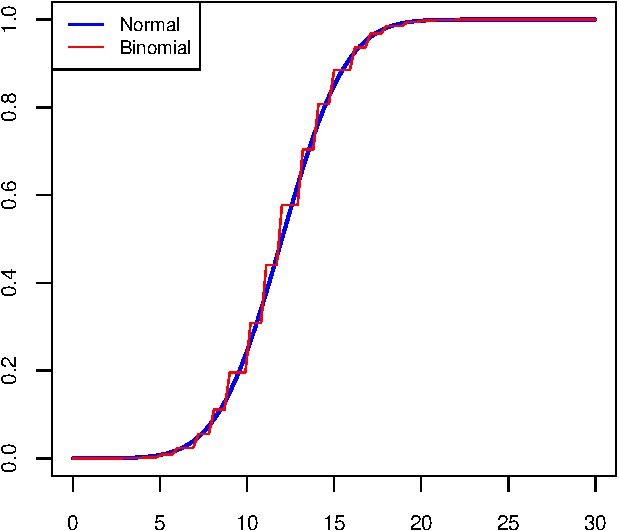
\includegraphics[width=0.8\linewidth]{Bioestadistica-II_files/figure-latex/unnamed-chunk-102-1} \end{center}

El gràfic següent mostra l'efecte combinat:

\begin{center}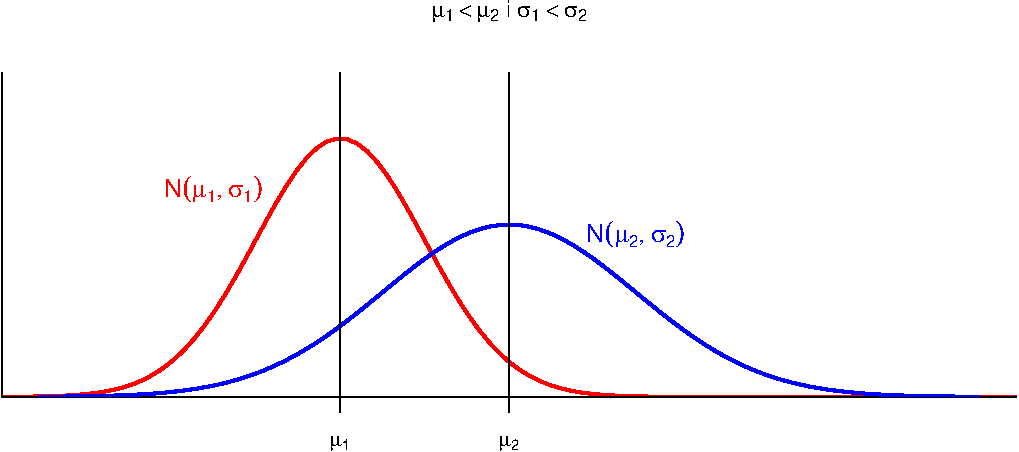
\includegraphics[width=0.8\linewidth]{Bioestadistica-II_files/figure-latex/unnamed-chunk-103-1} \end{center}

Indicarem amb \(z_q\) el \textbf{\(q\)-quantil} d'una variable normal estàndard \(Z\). És a dir, \(z_q\) és el valor tal que \(P(Z\leq z_q)=q\).

A banda del fet que \(z_{0.5}=0\) (la mediana de \(Z\) és 0), hi ha dos quantils més de la normal estàndard \(Z\) que hauríeu de recordar:

\begin{itemize}
\item
  \(z_{0.95}=1.64\); és a dir, \(P(Z\leq 1.64)=0.95\) i per tant \(P(Z\leq -1.64)=P(Z\geq 1.64)=0.05\) i
  \[
  P(-1.64\leq Z\leq 1.64)=0.9.
  \]
\item
  \(z_{0.975}=1.96\); és a dir, \(P(Z\leq 1.96)=0.975\) i per tant \(P(Z\leq -1.96)=P(Z\geq 1.96)=0.025\) i
  \[
  P(-1.96\leq Z\leq 1.96)=0.95.
  \]
\end{itemize}

\begin{rmdmercifulgod}
Molt sovint el valor 1.96 de \(z_{0.975}\) s'aproxima per 2. Teniu permís per a fer-ho quan no disposeu de mitjans (R, aplis de mòbil) per a calcular quantils i us considereu incapaços de recordar ``1.96''. Però només en aquest cas.
\end{rmdmercifulgod}

Una de les propietats de la distribució normal que ens faciliten molt la vida és que \textbf{tota combinació lineal de variables aleatòries normals independents és normal}. En concret, tenim els dos resultats següents:

\begin{theorem}
\protect\hypertarget{thm:comblinnormals}{}{\label{thm:comblinnormals} }Sigui \(X\) una variable \(N(\mu,\sigma)\).

\begin{enumerate}
\def\labelenumi{\arabic{enumi}.}
\item
  Per a tots \(a,b\in \mathbb{R}\), \(aX+b\) és normal \(N(a\mu+b,|a|\cdot\sigma)\).
\item
  En particular, la \textbf{tipificada} de \(X\)
  \[
  Z=\dfrac{X-\mu}{\sigma}
  \]
  és normal estàndard.
  \end{theorem}
\end{enumerate}

Més en general:

\begin{theorem}
\protect\hypertarget{thm:comblinnormals2}{}{\label{thm:comblinnormals2} }Si \(X_1,\ldots,X_n\) són variables aleatòries normals \textbf{independents} i \(a_1,\ldots,a_n,b\in \mathbb{R}\), llavors \(a_1X_1+\cdots +a_nX_n+b\) és \(N(\mu,\sigma)\) amb
\[
\mu=a_1\mu_1+\cdots +a_n\mu_n+b,\ 
\sigma=\sqrt{a_1^2\sigma^2_1+\cdots +a_n^2\sigma^2_n}
\]
\end{theorem}

\begin{rmdnote}
Que tota combinació lineal de variables normals torni a ser del mateix tipus, és a dir, normal, és una propietat molt útil de les variables normals que poques famílies de distribucions comparteixen. Per exemple, si \(X\) és una variable binomial \(B(n,p)\) amb \(p\neq 0\), la variable \(2X\) no és binomial, perquè només pren valors parells, mentre que una variable binomial \(B(m,q)\) ha de poder prendre tots els valors entre 0 i \(m\).
\end{rmdnote}

Les probabilitats de la normal tipificada determinen les de la normal original, perquè si \(X\) és \(N(\mu,\sigma)\):
\[
\begin{array}{rl}
P(a\leq X\leq b)\!\!\!\!\! & \displaystyle =P\Big( \frac{a-\mu}{\sigma}\leq \frac{X-\mu}{\sigma}\leq \frac{b-\mu}{\sigma}\Big)\\ & \displaystyle =P\Big(\frac{a-\mu}{\sigma}\leq Z\leq \frac{b-\mu}{\sigma}\Big)
\end{array}
\]
Això serveix per deduir fórmules, i els vostres pares ho empraven per calcular probabilitats de normals (amb taules de probabilitats de la normal estàndard); ara és més còmode usar una apli.

\hypertarget{intervals-de-referuxe8ncia}{%
\subsection{Intervals de referència}\label{intervals-de-referuxe8ncia}}

Un \textbf{interval de referència} del \(100q\%\) per a una variable aleatòria \(X\) és un interval \([a,b]\) tal que
\[
P(a\leq X\leq b)=q.
\]
És a dir, un interval de referència del \(100q\%\) per a \(X\) és un interval que conté els valors de \(X\) del \(100q\%\) dels subjectes de la població.

Per exemple, hem vist en la secció anterior que {[}-1.64,1.64{]} i {[}-1.96,1.96{]} són intervals de referència del 90\% i del 95\%, respectivament, per a una variable normal estàndard \(Z\).

Els més comuns són els intervals de referència del 95\% (\(q=0.95\)), que satisfan que
\[
P(a\leq X\leq b)=0.95
\]
i són els, que per exemple, us donen com a valors de referència en les analítiques:

\begin{center}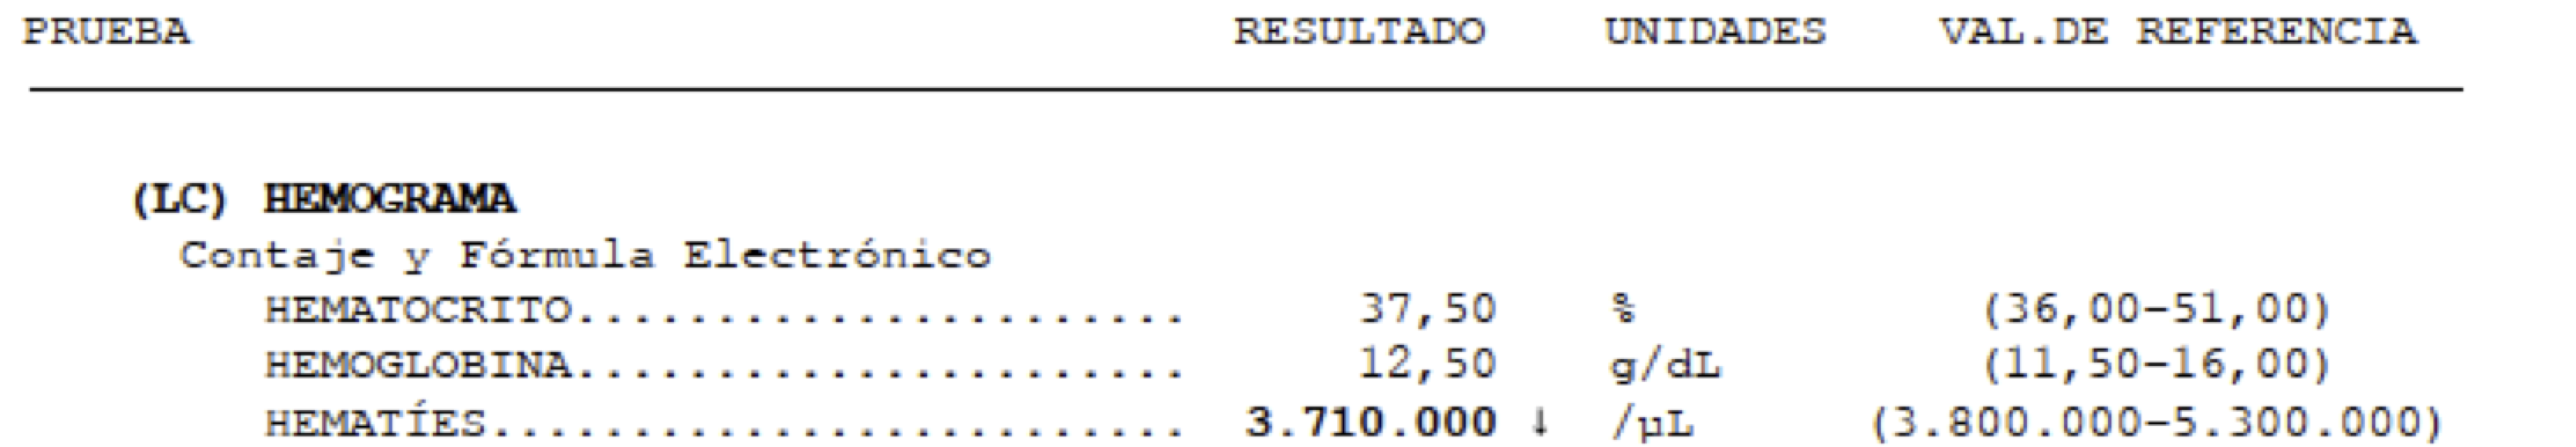
\includegraphics[width=0.8\linewidth]{Bioestadistica-II_files/figure-html/analit} \end{center}

\begin{rmdnote}
Quan es parla d'un \textbf{interval de referència} sense donar la probabilitat, se sobreentén sempre que és l'interval de referència del 95\%.
\end{rmdnote}

Quan \(X\) és \(N(\mu,\sigma)\), aquests intervals de referència es prenen sempre \textbf{centrats en la mitjana} \(\mu\), és a dir, de la forma
\[
[\mu-\text{alguna cosa},\mu+\text{aquesta mateixa cosa}].
\]
Es calculen amb el resultat següent:

\begin{theorem}
\protect\hypertarget{thm:unnamed-chunk-108}{}{\label{thm:unnamed-chunk-108} }Si \(X\) és \(N(\mu,\sigma)\), un interval de referència del \(100q\%\) per a \(X\) és
\[
[\mu- z_{(1+q)/2}\cdot \sigma, \mu+ z_{(1+q)/2}\cdot \sigma]
\]
on \(z_{(1+q)/2}\) indica el \((1+q)/2\)-quantil de la normal estàndard \(Z\). Normalment escriurem aquest interval
\[
\mu\pm z_{(1+q)/2}\cdot \sigma.
\]
\end{theorem}

\begin{rmdcorbes}
La demostració és un exemple d'ús de la tipificació de la normal:
\[
\begin{array}{l}
P(\mu-x\leq X\leq \mu+x)=q\\
\qquad \Longleftrightarrow \displaystyle P\Big(\frac{\mu-x-\mu}{\sigma}\leq \frac{X-\mu}{\sigma}\leq \frac{\mu+x-\mu}{\sigma}\Big)=q\\
\qquad \Longleftrightarrow \displaystyle P(-x/{\sigma}\leq Z\leq {x}/{\sigma})=q\\
\qquad \Longleftrightarrow \displaystyle P(Z\leq {x}/{\sigma})-P(Z\leq -{x}/{\sigma})=q\\
\qquad \Longleftrightarrow \displaystyle P(Z\leq {x}/{\sigma})-(1-P(Z\leq {x}/{\sigma}))=q\\
\qquad \text{(per la simetria de $f_Z$ al voltant de 0)}\\
\qquad \Longleftrightarrow \displaystyle 2P(Z\leq {x}/{\sigma})=q+1\\
\qquad \Longleftrightarrow P(Z\leq {x}/{\sigma})=(1+q)/2\\
\qquad \Longleftrightarrow x/\sigma=
z_{(1+q)/2}\\
\qquad \Longleftrightarrow x=z_{(1+q)/2}\cdot \sigma
\end{array}
\]
\end{rmdcorbes}

Si \(q=0.95\), llavors \((1+q)/2=0.975\) i \(z_{0.975}=1.96\). Per tant, l'interval de referència del 95\% per a una variable \(X\) normal \(N(\mu,\sigma)\) és
\[
\mu\pm 1.96\sigma.
\]
I com que aquest 1.96 sovint s'aproxima per 2, l'interval de referència del 95\% d'una \(N(\mu,\sigma)\) se sol simplificar a
\[
\mu\pm 2\sigma.
\]
Això diu, bàsicament, que

\begin{quote}
Si una població segueix una distribució normal \(N(\mu,\sigma)\), un 95\% dels seus individus tenen el seu valor de \(X\) a distància com a màxim \(2\sigma\) (``a dues sigmes'') de \(\mu\).
\end{quote}

\begin{example}
\protect\hypertarget{exm:unnamed-chunk-110}{}{\label{exm:unnamed-chunk-110} }Segons l'OMS, les altures (en cm) de les dones europees de 18 anys segueixen una llei \(N(163.1,18.53)\). Quin és l'interval d'altures centrat en la mitjana que conté a la meitat les europees de 18 anys?
\end{example}

Fixau-vos que, si diem \(X\) a la variable aleatòria ``Altura d'una dona europea de 18 anys en cm'', el que volem saber és l'interval centrat en la seva mitjana, 163.1, tal que la probabilitat que l'alçada d'una europea de 18 anys triada a l'atzar pertanyi a aquest interval sigui 0.5. És a dir, l'interval de referència del 50\% per a \(X\).

Ens diuen que \(X\) és \(N(163.1,18.53)\). Si \(q=0.5\), llavors \((1+q)/2=0.75\). El 0.75-quantil \(z_{0.75}\) d'una normal estàndard és

\begin{Shaded}
\begin{Highlighting}[]
\FunctionTok{qnorm}\NormalTok{(}\FloatTok{0.75}\NormalTok{)}
\end{Highlighting}
\end{Shaded}

\begin{verbatim}
## [1] 0.6744898
\end{verbatim}

Per tant, l'interval de referència demanat és \(163.1\pm 0.6745\cdot 18.53\), és a dir, arrodonint a mm, \([150.6, 175.6]\). Això ens diu que la meitat de les dones europees de 18 anys fan entre 150.6 i 175.6 cm.

El \textbf{z-score} d'un valor \(x_0\in \mathbb{R}\) respecte d'una distribució \(N(\mu,\sigma)\) és
\[
\frac{x_0-\mu}{\sigma}
\]

És a dir, el z-score de \(x_0\) és el resultat de ``tipificar'' \(x_0\) en el sentit del Teorema \ref{thm:comblinnormals}.2.

Si la variable poblacional és normal, com més gran és el valor absolut del z-score de \(x_0\), més ``rar'' és \(x_0\); el signe ens diu si és més gran o més petit que el valor esperat \(\mu\).

\begin{example}
\protect\hypertarget{exm:unnamed-chunk-112}{}{\label{exm:unnamed-chunk-112} }Recordau que, segons l'OMS, les altures de les dones europees de 18 anys segueixen una llei \(N(163.1,18.53)\). Quin seria el z-score d'una jugadora de bàsquet de 18 anys que fes 191 cm?
\end{example}

Seria
\[ 
\frac{191-163.1}{18.53}=1.5
\]

Això se sol llegir dient que l'alçada d'aquesta jugadora està \textbf{1.5 sigmes per sobre de l'alçada mitjana}.

\hypertarget{variables-log-normals}{%
\subsection{Variables log-normals}\label{variables-log-normals}}

Direm que \(X\) és una variable \red{log-normal} quan el seu logaritme \(\ln(X)\) és una variable normal. O, si ho preferiu, és una variable de la forma \(e^Y\) amb \(Y\) normal. Moltes concentracions d'enzims o anticossos tenen distribució aproximadament log-normal.

La densitat d'una variable log-normal és asimètrica, amb una cua a la dreta, com mostra la Figura \ref{fig:lognorm}.

\begin{figure}

{\centering 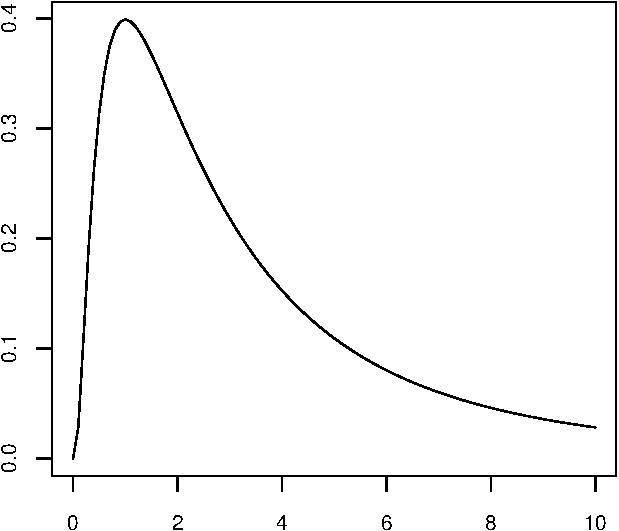
\includegraphics[width=0.5\linewidth]{Bioestadistica-II_files/figure-latex/lognorm-1} 

}

\caption{Densitat de $e^Z$ amb $Z$ normal estàndard.}\label{fig:lognorm}
\end{figure}

Recíprocament, molt sovint una variable la densitat de la qual mostri una pujada ràpida des del 0 a la moda i després una cua a la dreta, satisfà que el seu logaritme segueix una distribució aproximadament normal. Això serà útil més endavant.

Amb R, la distribució log-normal és \texttt{lognorm}. Els paràmetres que s'empren per descriure-la són els de la variable normal definida pel seu logaritme:

\begin{itemize}
\item
  La \emph{mitjana en escala logarítmica} de \(X\): \(\mu_{\ln(X)}\)
\item
  La \emph{desviació típica en escala logarítmica} de \(X\): \(\sigma_{\ln(X)}\)
\end{itemize}

\hypertarget{test-de-la-lliuxe7uxf3-1}{%
\section{Test de la lliçó 1}\label{test-de-la-lliuxe7uxf3-1}}

\hypertarget{variables-aleatuxf2ries-discretes-1}{%
\subsection{Variables aleatòries discretes}\label{variables-aleatuxf2ries-discretes-1}}

\textbf{(1)} Sigui \(X\) una variable aleatòria discreta de mitjana \(\mu\) i desviació típica \(\sigma\). Quina o quines de les afirmacions següents són sempre vertaderes?

\begin{enumerate}
\def\labelenumi{\arabic{enumi}.}
\tightlist
\item
  \(E(X+2)=\mu+2\).
\item
  \(\sigma(X+2)=\sigma+2\).
\item
  \(\sigma(-X)=-\sigma\).
\item
  \(\sigma(-X)=\sigma\).
\item
  \(\sigma(X/2)=\sigma/2\).
\item
  Cap de les altres afirmacions és vertadera.
\end{enumerate}

\textbf{(2)} La funció de distribució \(F_X(x)\) d'una variable aleatòria \(X\) ens dóna:

\begin{enumerate}
\def\labelenumi{\arabic{enumi}.}
\tightlist
\item
  La probabilitat d'obtenir el valor \(x\).
\item
  La probabilitat d'obtenir un valor entre \(-x\) i \(x\), tots dos extrems inclosos.
\item
  La probabilitat d'obtenir un valor entre \(0\) i \(x\), tots dos extrems inclosos.
\item
  La probabilitat d'obtenir un valor més petit o igual que \(x\).
\item
  La probabilitat d'obtenir un valor estrictament més petit que \(x\).
\end{enumerate}

\textbf{(3)} El nombre anual d'accidents laborals d'un tipus concret segueix una distribució de Poisson. Al llarg del temps s'ha observat que el 55\% dels anys no es produeix cap accident d'aquests. Quin valor estimes que té el paràmetre \(\lambda\) d'aquesta distribució de Poisson?

\begin{enumerate}
\def\labelenumi{\arabic{enumi}.}
\tightlist
\item
  0.55
\item
  \(e^{-0.55}\)
\item
  \(\ln(0.55)\)
\item
  \(-\ln(0.55)\)
\item
  Un valor que no és cap dels proposats en les altres respostes.
\end{enumerate}

\textbf{(4)} Quina o quines de les variables següents tenen distribució binomial?

\begin{enumerate}
\def\labelenumi{\arabic{enumi}.}
\tightlist
\item
  El pes d'una persona triada a l'atzar.
\item
  Triam un nombre de llançaments a l'atzar, llançam aquest nombre de vegades una moneda, i comptam el nombre de cares.
\item
  El nombre de glòbuls vermells en 1 mm\textsuperscript{3} de sang.
\item
  La proporció d'hipertensos en una mostra aleatòria de 50 individus.
\item
  Triam 10 estudiants diferents en una classe de 20, i comptam quantes dones han sortit.
\item
  Cap d'elles.
\end{enumerate}

\textbf{(5)} Quina o quines de les variables següents tenen una distribució de Poisson?

\begin{enumerate}
\def\labelenumi{\arabic{enumi}.}
\tightlist
\item
  El pes d'una persona triada a l'atzar.
\item
  El nombre de casos diaris de COVID-19 a Mallorca.
\item
  El nombre de glòbuls vermells en 1 mm\textsuperscript{3} de sang.
\item
  La proporció d'hipertensos en una mostra aleatòria de 50 individus.
\item
  Triam 10 estudiants diferents en una classe de 20, i comptam quantes dones han sortit.
\end{enumerate}

\hypertarget{variables-aleatuxf2ries-contuxednues-1}{%
\subsection{Variables aleatòries contínues}\label{variables-aleatuxf2ries-contuxednues-1}}

\textbf{(6)} Sigui \(X\) una variable aleatòria contínua de funció de densitat:
\[
f_X(x)=\left\{\begin{array}{ll}
0 & \mbox{si $x<0$}\\
\frac{2\sqrt{2}}{\sqrt{\pi}} e^{-2x^2} & \mbox{si $x\geq 0$}
\end{array}
\right.
\]
És cert que \(P(X=1)=2\sqrt{2}e^{-2}/\sqrt{\pi}\)?

\begin{enumerate}
\def\labelenumi{\arabic{enumi}.}
\tightlist
\item
  Sí
\item
  No: en realitat \(P(X=1)=\int_{-\infty}^1 \frac{2\sqrt{2}}{\sqrt{\pi}} e^{-2x^2}\,dx\) però no sé calcular aquesta integral, o sí que sé calcular-la, però em fa mandra fer-ho.
\item
  Això no és la funció de densitat d'una variable aleatòria contínua, perquè no és una funció contínua (en el 0 bota de 0 a \(2\sqrt{2}/\sqrt{\pi}\))
\item
  Totes les altres respostes són incorrectes
\end{enumerate}

\textbf{(7)} Sigui \(X\) una variable aleatòria contínua de mitjana \(\mu\). Què val \(P(X=\mu)\)?

\begin{enumerate}
\def\labelenumi{\arabic{enumi}.}
\tightlist
\item
  0.5
\item
  \(\mu\)
\item
  0
\item
  Depèn de la variable aleatòria
\item
  Totes les altres respostes són falses
\end{enumerate}

\textbf{(8)} Sigui \(X\) una variable aleatòria contínua de moda \(M\). Què val \(P(X=M)\)?

\begin{enumerate}
\def\labelenumi{\arabic{enumi}.}
\tightlist
\item
  1
\item
  0.5
\item
  0
\item
  Depèn de la variable aleatòria, però és el valor màxim de \(P(X=x)\)
\item
  Depèn de la variable aleatòria, però és el valor màxim de la funció de densitat de \(X\).
\item
  Totes les altres respostes són falses
\end{enumerate}

\textbf{(9)} Sigui \(Z\) una variable aleatòria normal estàndard. Marca les afirmacions vertaderes.

\begin{enumerate}
\def\labelenumi{\arabic{enumi}.}
\tightlist
\item
  És asimètrica a l'esquerra.
\item
  La seva mitjana és 1.
\item
  La seva desviació típica és 0.
\item
  La seva variància és 1.
\item
  La seva mitjana és 0.
\end{enumerate}

\textbf{(10)} Sigui \(X\) una variable aleatòria \(N(\mu,\sigma)\) i \(f_X\) la seva funció de densitat. Què val l'àrea entre la corba \(y=f_X(x)\) i l'eix d'abscisses?

\begin{enumerate}
\def\labelenumi{\arabic{enumi}.}
\tightlist
\item
  0
\item
  \(\mu\)
\item
  \(\sigma\)
\item
  1
\item
  Totes les altres respostes són falses
\end{enumerate}

\textbf{(11)} Siguin \(X\) una variable aleatòria \(N(\mu,\sigma)\) i \(f_X\) la seva funció de densitat. Quina de les afirmacions següents és vertadera?

\begin{enumerate}
\def\labelenumi{\arabic{enumi}.}
\tightlist
\item
  \(\mu\) és la mitjana de \(X\), però no la seva mediana
\item
  \(\mu\) és la mitjana i la mediana de \(X\), però no la seva moda
\item
  \(\mu\) és la mitjana, la mediana i la moda de \(X\), però no és veritat que \(P(X=\mu)>P(X=a)\) per a tot \(a\neq \mu\)
\item
  \(\mu\) és la mitjana, la mediana i la moda de \(X\) i \(P(X=\mu)>P(X=a)\) per a tot \(a\neq \mu\)
\end{enumerate}

\textbf{(12)} El FME (Flux Màxim d'Expiració) de les al·lotes d'11 anys segueix una distribució aproximadament normal de mitjana 300 l/min i desviació típica 20 l/min. Marca les afirmacions vertaderes:

\begin{enumerate}
\def\labelenumi{\arabic{enumi}.}
\tightlist
\item
  Aproximadament la meitat de les al·lotes d'11 anys tenen un FME entre 280 l/min i 320 l/min.
\item
  Al voltant del 95\% de les al·lotes d'11 anys tenen un FME entre 280 l/min i 320 l/min.
\item
  Al voltant del 95\% de les al·lotes d'11 anys tenen un FME entre 260 l/min i 340 l/min.
\item
  Al voltant del 5\% de les al·lotes d'11 anys tenen un FME inferior a 260 l/min.
\item
  Cap al·lota d'11 anys té FME superior a 360 l/min.
\end{enumerate}

\textbf{(13)} En una mostra aleatòria extreta de població sana es troba que una variable bioquímica té com a mitjana 90 i desviació típica 10. Si prenem una mostra d'individus sans, és raonable esperar que aproximadament el 95\% d'ells tenguin un valor d'aquesta variable comprès entre 70 i 110? (marca totes les respostes correctes):

\begin{enumerate}
\def\labelenumi{\arabic{enumi}.}
\tightlist
\item
  Sí, sempre.
\item
  No, mai.
\item
  Si la variable té distribució normal, sí.
\item
  Si la mostra és prou gran, sí.
\item
  Si la variable té distribució normal i la mostra és prou gran, sí.
\end{enumerate}

\textbf{(14)} En una variable aleatòria contínua, la seva funció de densitat (marca una sola resposta):

\begin{enumerate}
\def\labelenumi{\arabic{enumi}.}
\tightlist
\item
  És sempre contínua
\item
  Mesura el dens que és el seu domini.
\item
  Aplicada a un nombre real, ens dóna dóna la probabilitat d'obtenir aquest número.
\item
  Aplicada a un nombre real, ens dóna la probabilitat d'obtenir un valor menor o igual que aquest número.
\item
  Totes les altres respostes són falses
\end{enumerate}

\textbf{(15)} Sigui \(X\) una variable aleatòria contínua de desviació típica \(\sigma\). Què val la variància de la variable aleatòria \(-X/2\)?

\begin{enumerate}
\def\labelenumi{\arabic{enumi}.}
\tightlist
\item
  \(\sigma(-X/2)^2=-\sigma^2/2\).
\item
  \(\sigma(-X/2)^2=\sigma^2/2\).
\item
  \(\sigma(-X/2)^2=-\sigma^2/4\).
\item
  \(\sigma(-X/2)^2=\sigma^2/4\).
\item
  Totes les altres respostes són falses
\end{enumerate}

\textbf{(16)} Sigui \(Z\) una variable aleatòria normal estàndard. Marca totes les afirmacions vertaderes.

\begin{enumerate}
\def\labelenumi{\arabic{enumi}.}
\tightlist
\item
  És asimètrica a l'esquerra.
\item
  La seva mitjana és 1.
\item
  La seva desviació típica és 0.
\item
  La seva variància és 1.
\item
  La seva mediana és 0.
\end{enumerate}

\textbf{(17)} El temps que tarda a produir-se una determinada reacció bioquímica es distribueix segons una variable normal de mitjana 17 minuts i desviació típica 3 minuts. Què podem deduir d'aquesta afirmació? Marca totes les respostes correctes:

\begin{enumerate}
\def\labelenumi{\arabic{enumi}.}
\tightlist
\item
  Tots aquests temps se situen entre 8 i 26 minuts.
\item
  Gairebé tots aquests temps se situen entre 11 i 23 minuts.
\item
  És estrictament més probable que una reacció d'aquestes tardi entre 16 i 18 minuts que tardi entre 18 i 20 minutos.
\item
  És estrictament més probable que una reacció d'aquestes tardi entre 18 i 20 minutos que tardi entre 16 i 18 minuts.
\item
  És estrictament més probable que una reacció d'aquestes tardi entre 18 i 20 minutos que tardi entre 14 i 16 minuts.
\item
  Cap de les afirmaciónes anteriors és correcta.
\end{enumerate}

\textbf{(18)} El temps que tarda a produir-se una determinada reacció bioquímica es distribueix segons una variable normal de mitjana 17 minuts i desviació típica 3 minuts. Quina és la probabilitat que tardi menys de 17 minuts?

\begin{enumerate}
\def\labelenumi{\arabic{enumi}.}
\tightlist
\item
  0
\item
  0.5
\item
  1
\item
  17/3
\item
  17/2
\item
  Cap de les afirmaciónes anteriors és correcta.
\end{enumerate}

\textbf{(19)} El temps que tarda a produir-se una determinada reacció bioquímica es distribueix segons una variable normal de mitjana 17 minuts i desviació típica 3 minuts. Quina o quines de les afirmacions següents són vertaderes?

\begin{enumerate}
\def\labelenumi{\arabic{enumi}.}
\tightlist
\item
  Si poguéssim mesurar els temps amb precisió infinita, observaríem que el temps que tarda més sovint és exactament 17 minuts.
\item
  Arrodonint a segons, el temps que tarda més sovint és 17 minuts.
\item
  En un 95\% de les ocasions tarda aproximadament entre 14 i 20 minutos
\item
  Tarda més de 20 minutos amb la mateixa freqüència amb la qual tarda menys de 14 minuts
\item
  Tarda més de 20 minutos amb la mateixa freqüència amb la qual tarda menys de 20 minutos
\item
  En un 95\% de les ocasions tarda 23 minuts o menys
\end{enumerate}

\textbf{(20)} Quina de les tres afirmacions és vertadera per a les tres distribucions normals de la figura inferior? (\(\sigma_1\), \(\sigma_2\) i \(\sigma_3\) indiquen les desviacions típiques de les corbes 1, 2 i 3, respectivament).

\begin{enumerate}
\def\labelenumi{\arabic{enumi}.}
\item
  \(\sigma_1> \sigma_2> \sigma_3\)
\item
  \(\sigma_1< \sigma_2< \sigma_3\)
\item
  \(\sigma_1= \sigma_2= \sigma_3\)
\item
  Del gràfic no es pot deduir la relació entre les tres desviacions típiques
\item
  Cap de les altres afirmacions és veritable.
\end{enumerate}

\begin{center}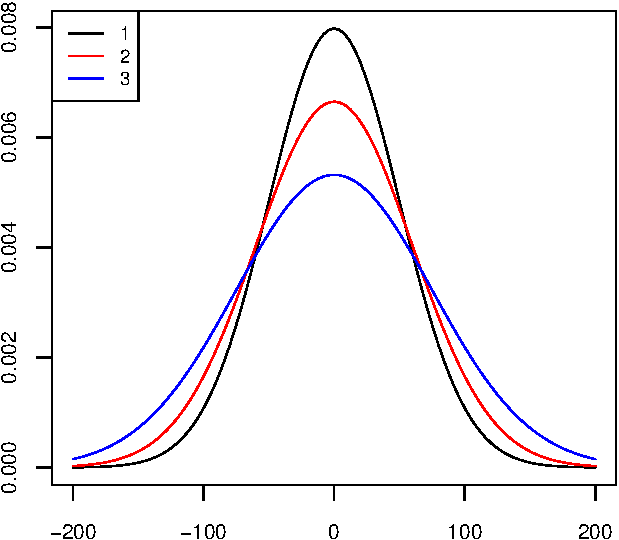
\includegraphics[width=0.5\linewidth]{Bioestadistica-II_files/figure-latex/unnamed-chunk-113-1} \end{center}

\textbf{(21)} El pes mitjà d'una bossa de patates d'una determinada marca és de 150 grams amb una desviació típica de 5.6 grams. Quin és el z-score d'una bossa que pesa 147 grams (arrodonit a 2 xifres decimals)?

\begin{enumerate}
\def\labelenumi{\arabic{enumi}.}
\tightlist
\item
  \(-0.54\)
\item
  0.30\%
\item
  0.54\%
\item
  0.70\%
\item
  Cap de les respostes anteriors és correcta
\end{enumerate}

\textbf{(22)} Si una v.a. normal té mitjana 18.1 i desviació típica 1.2, què val el seu 3er quartil (arrodonit a una xifra decimal)? (Pots usar R per calcular-lo)

\begin{enumerate}
\def\labelenumi{\arabic{enumi}.}
\tightlist
\item
  18.1\%
\item
  18.9
\item
  19.3\%
\item
  20.5\%
\item
  Cap de les respostes anteriors és correcta
\end{enumerate}

\textbf{(23)} L'interval de referència (del 95\%) de la concentració de creatinina en sèrum és 0.66-1.09 mg/dl. Què en podem deduir? (Marca només una resposta.)

\begin{enumerate}
\def\labelenumi{\arabic{enumi}.}
\item
  Que la probabilitat que la concentració mitjana de creatinina en sèrum estigui entre 0.66 i 1.09 mg/dl és del 95\%.
\item
  Que si prenem una mostra aleatòria d'individus i calculem la mitjana de les seves concentracions de creatinina, en un 95\% de les ocasions aquesta mitjana estarà entre 0.66 i 1.09 mg/dl.
\item
  Que un 5\% dels individus tenen una concentració de creatinina en sèrum superior a 1.09 mg/dl.
\item
  Que un 95\% dels individus tenen una concentració de creatinina en sèrum entre 0.66 i 1.09 mg/dl.
\item
  Que si prenem una mostra aleatòria d'individus, en un 95\% de les ocasions tots els valors estaran entre 0.66 i 1.09 mg/dl.
\item
  Cap de les altres respostes és correcta.
\end{enumerate}

\end{document}
